%!TeX program = lualatex

\documentclass[oneside]{academica}
\usetikzlibrary{automata,positioning,trees,patterns} % for automata and trees
\usepackage{diagbox} % for boxes
\usepackage{scalerel} % for scaling symbols
\usepackage{stmaryrd} % for llbracket

\setlength{\parindent}{0pt}

\hyphenation{ta-bleau}
\hyphenation{ta-bleaux}

\newcommand{\wlogt}{w.l.o.g.\xspace}
\newcommand{\Wlogt}{W.l.o.g.\xspace}

\newcommand{\DBA}{\tuple{Q, A, \d, q_0, F}}
\newcommand{\NBA}{\tuple{Q, A, \D, q_0, F}}
\newcommand{\DMA}{\tuple{Q, A, \d, q_0, \F}}
\newcommand{\NMA}{\tuple{Q, A, \D, q_0, \F}}
\newcommand{\DRA}{\tuple{Q, A, \d, q_0, \O}}
\newcommand{\NRA}{\tuple{Q, A, \D, q_0, \O}}

\newcommand{\Aw}{A^\w}

%\newcommand{\eNFA}{{{$\varepsilon$}-NFA\xspace}}
\newcommand{\eNFA}{{e-NFA\xspace}}

\newcommand{\Buchi}{B\"{u}chi\xspace}
\newcommand{\wword}{$\w$-word\xspace}
\newcommand{\wwords}{$\w$-words\xspace}
\newcommand{\wclo}{$\w$-closure\xspace}
\newcommand{\wlan}{$\w$-language\xspace}
\newcommand{\wlans}{$\w$-languages\xspace}
\newcommand{\wreg}{$\w$-regular\xspace}

\newcommand{\SA}{$\text{S1S}_A$\xspace}

\renewcommand{\succ}{\text{succ}}
\newcommand{\succxy}{\succ(X,Y)}
\newcommand{\tsuc}{$\t$-successor\xspace}

\newcommand{\sing}[1]{\text{sing}(#1)}

\renewcommand{\inf}[1]{\text{Inf}(#1)}
\newcommand{\infs}{\inf{\sigma}}

\newcommand{\eqn}{\equiv_{n}}
\newcommand{\eqnn}{\equiv_{(n,1)}}

\newcommand{\px}{\p(x)}

\newcommand{\Twa}{T^\w_A}

\newcommand{\AP}{{\mathcal{AP}}}
\newcommand{\sAP}{(2^{\AP})^\w}

\newcommand{\wY}{{\tilde{Y}}}
\newcommand{\state}[1]{\text{state}(#1)}

\newcommand{\bgraph}{\B_{(\P,\p)}}

\newcommand{\mcirc}{{\mathbin{\scalerel*{\bigcirc}{gX}}}}
\newcommand{\msquare}{{\mathbin{\scalerel*{\square}{gX}}}}

\renewcommand{\emptyset}{\varnothing}

\newcommand{\XX}{\mathrm{X}}
\newcommand{\UU}{\mathrm{U}}
\newcommand{\RRR}{\mathrm{R}}
\newcommand{\EE}{\mathrm{E}}
\renewcommand{\AA}{\mathrm{A}}
\newcommand{\FF}{\mathrm{F}}
\newcommand{\GG}{\mathrm{G}}
\newcommand{\EX}{\mathrm{EX}}
\newcommand{\AX}{\mathrm{AX}}
\newcommand{\EU}{\mathrm{EU}}
\newcommand{\AU}{\mathrm{AU}}
\newcommand{\EF}{\mathrm{EF}}
\newcommand{\AF}{\mathrm{AF}}
\newcommand{\EG}{\mathrm{EG}}
\newcommand{\AG}{\mathrm{AG}}
\newcommand{\FG}{\mathrm{FG}}
\newcommand{\GF}{\mathrm{GF}}

\newcommand{\ol}[1]{\,\overline{\!{#1}}}
\newcommand{\ul}[1]{\,\underline{{#1}\!}}
%\newcommand{\oa}[1]{\overrightarrow{{#1}\!}}

\newcommand{\lLk}{{}_l L_k}
\newcommand{\kloop}[1]{\llbracket {#1} \rrbracket_k}
\newcommand{\kloopl}[1]{{}_l \llbracket {#1} \rrbracket_k}
\newcommand{\kloopil}[1]{{}_l \llbracket {#1} \rrbracket^i_k}
\newcommand{\kloopsl}[1]{{}_l \llbracket {#1} \rrbracket^{\succ(i)}_k}

\newcommand{\var}{\text{var}}
\newcommand{\val}{\text{value}}
\newcommand{\low}{\text{low}}
\newcommand{\high}{\text{high}}

\newcommand{\attr}{\text{Attr}}


\overtitle{notes for}
\title{Verification and Validation}
\author{Merlo Filippo}

\begin{document}

\frontmatter

\maketitle

\tableofcontents

\mainmatter

\chapter{Basics}

\begin{note}[Roadmap of the course]
  These notes tell one connected story: how to \emph{specify} the behavior of computational systems, and how to \emph{verify} that behavior algorithmically. The thread we follow is
  \begin{center}
    automata $\to$ transition systems $\to$ logical specifications $\to$ temporal logic $\to$ model checking $\to$ state explosion $\to$ symbolic representation (OBDDs) $\to$ synthesis and monitoring.
  \end{center}
  The hidden backbone tying the chapters together is a single chain of equivalences: the languages of infinite words called \wreg are exactly those recognized by \Buchi/Muller/Rabin automata, exactly those definable in the logic S1S (\Buchi's theorem), and -- for their first-order fragment -- exactly those expressible in LTL (Kamp's theorem). Model checking, symbolic methods, synthesis and monitoring are all algorithmic ways of exploiting this one correspondence. Each chapter states \emph{which problem it solves} and \emph{what it hands to the next}; keep this map in mind.
\end{note}

\section{Introduction}

A \textbf{tautology} is a formula which is valid in every structure/interpretation. A \textbf{contradiction} is the opposite, no matter the interpretation, is always false, and we call the formula unsatisfiable.

There are two types of variables:
\begin{itemize}
  \item \textbf{first-order}, which represent single elements and references via a lowercase character (\eg, $x,y,z$);
  \item \textbf{second-order}, which represent finite/infinite sets of single elements and noted with an uppercase character (\eg, $Y_\text{finite}, Z_\text{infinite}$).
\end{itemize}

Logic is a language used to express the following properties:
\begin{itemize}
  \item \textbf{vocabulary}: the set of symbols used to create formulas;
  \item \textbf{syntax}: the rules to follow when combining symbols;
  \item \textbf{semantics}: the meaning of formulas.
\end{itemize}

\begin{definition*}[Reduction]
  A \textbf{reduction} $\leq$ from a problem $P$ to another $Q$ it's algorithm $F$ that solves $P$ using a solution for $Q$ as oracle:
  \begin{equation*}
    \forall x P(x) \iff Q\left(F(x)\right)
  \end{equation*}
  \ie, if we're able to solve $Q$ it means that we also can solve $P$, or that solving $P$ cannot be computationally harder than solving $Q$.
\end{definition*}

The order of time and space complexity sets is
\begin{equation*}
  \text{P} \subseteq \text{NP} \subseteq \text{PSPACE} \subseteq \text{EXP} \subseteq \dots
\end{equation*}
where
\begin{itemize}
  \item an algorithm belongs to P if it's computable in polynomial \textit{TIME} with a deterministic machine;
  \item an algorithm belongs to NP if it's computable in polynomial \textit{TIME} with a \emph{non}-de\-ter\-mi\-ni\-stic machine;
  \item an algorithm belongs to PSPACE if its computation takes up polynomial \textit{SPACE} with a deterministic machine.
\end{itemize}

\textit{Expressiveness} vs. \textit{Decidability} - more expressive means also possibly undecidable.

\textit{Succinctness} vs. \textit{Efficiency} - the more symbols are used in a logic, the less efficient will be to evaluates that logic.

\textbf{Normal forms}, are standard formula structures used to simplify the logic.
An \textbf{algebraic representation} is a different representation of a logic formula, which aim to maintain the same low-level formalism but with a different representation, more useful in a different context.

Some crucial decision problems are:
\begin{itemize}
  \item \textbf{model-checking}: given a formula $\p$ and a structure $S$, decide if $S \models \p$, \ie, if $\p$ holds for $S$ or, equally, if $S$ makes $\p$ \true.
  \item \textbf{validity/satisfiability}:
    \begin{itemize}
      \item[] \textit{validity} \quad given a formula $\p$, decide if $\p$ holds for all possible $S$;
      \item[] \textit{satisfiability} \quad given a formula $\p$, decide if it exists a structure $S$ that $\p$ holds for it.
    \end{itemize}
  \item \textbf{logical equivalence}: given two formulas $\p_1, \p_2$, decide whether $S \models \p_1 \iff S \models \p_2$ holds for all structures $S$. Equivalence reduces to validity ($\textsc{EQ} \le \textsc{VAL}$): $\p_1 \leftrightarrow \p_2$ is valid exactly when $\p_1$ and $\p_2$ are equivalent, so any decision procedure for validity also decides equivalence.
  \item \textbf{definability between logics}: given a formula $\p_1$ in $L_1$, decide if there is a $\p_2$ in $L_2$ logically equivalent to $\p_1$.
\end{itemize}

\newpage

\section{Logic}

\subsection{Propositional logic}

It's based on:
\begin{itemize}
  \item a \textbf{vocabulary}, that consists of 
    \begin{itemize}
      \item[] boolean variables, \eg, $\S = \set{p,q,r,\dots}$
      \item[] boolean connectives, \eg, $\land,\lor,\neg,\to,\leftrightarrow$
    \end{itemize}
  \item the \textbf{syntax}, which defines how vocabulary elements can be combined, \eg, $\p = p \mid q \mid \p \lor \p \mid \dots$
  \item the \textbf{semantic}, which describes when a structure $S \models \p$, \eg, given $S \in \S \implies \{\,\true,\allowbreak \false\,\}$:
    \begin{equation*}
      S \models \p \iff S(p) = \true
    \end{equation*}
\end{itemize}

\begin{lemma*}
  Every formula is equivalent to one without $\to$ and $\leftrightarrow$. In fact
  \begin{align*}
    \p_1 \to \p_2 \qquad &\iff \qquad \neg \p_1 \lor \p_2 \\
    \p_1 \leftrightarrow \p_2 \qquad &\iff \qquad (\neg \p_1 \lor \p_2) \land (\neg \p_2 \lor \p_1)
  \end{align*}
\end{lemma*}

\begin{definition*}[Negation Normal Form]
  \vspace{-15pt}
  \begin{align*}
    \p &= \p \lor \p \mid \p \land \p \mid a \\
    a &= p \mid \neg p
  \end{align*}
\end{definition*}

\begin{lemma*}
  Every formula is equivalent to one in \textbf{Negation Normal Form}. In fact
  \begin{align*}
    \neg(\p_1 \lor \p_2) \qquad &\iff \qquad \neg \p_1 \land \neg \p_2\\
    \neg(\p_1 \land \p_2) \qquad &\iff \qquad \neg \p_1 \lor \neg \p_2
  \end{align*}
\end{lemma*}

\begin{definition*}[Conjunctive Normal Form]
  \vspace{-15pt}
  \begin{align*}
    \p &= \p \land \p \mid a \\
    a &= a \lor a \mid p \mid \neg p
  \end{align*}
  and an example is
  \begin{equation*}
    (p_1 \lor p_2 \lor p_3) \land (p_4 \lor \ldots \lor p_i) \land \ldots \land (\ldots \lor \ldots \lor) 
  \end{equation*}

  The opposite of this notation is the \textbf{Disjunctive Normal Form}.
\end{definition*}

\begin{corollary}[Tseitin]\label{thm:tseitin}
  Every formula is equi-satisfiable to one in \textbf{Conjunctive Normal Form}. In fact
  \begin{align*}
    \neg(\p_1 \lor \p_2) \qquad &\iff \qquad \neg \p_1 \land \neg \p_2\\
    \neg(\p_1 \land \p_2) \qquad &\iff \qquad \neg \p_1 \lor \neg \p_2
  \end{align*}
\end{corollary}

\begin{proof*}[\nameref{thm:tseitin}]
  Take any $\p$ w.l.o.g.\footnote{without loss of generality} in NNF\footnote{Negation Normal Form}, \eg,
  \begin{equation*}
    \p = ((p \land \neg q) \lor \neg p) \land r \to \neg q,
  \end{equation*}
  it is equivalent to its CNF.

  Therefore,
  \vspace{-10pt}
  \begin{align*}
    \p &\equiv ((p \land \neg q) \lor \neg p) \land r \to \neg q\\
    &\equiv \neg (((p \land \neg q) \lor \neg p) \land r) \lor \neg q\\
    &\equiv \neg ((p \land \neg q) \lor \neg p) \lor \neg r \lor \neg q\\
    &\equiv (\neg (p \land \neg q) \land p) \lor \neg r \lor \neg q\\
    &\equiv ((\neg p \lor q) \land p) \lor \neg r \lor \neg q
  \end{align*}
  Now to transform leftmost part of $\p$ into CNF we need to introduce a new variable $z$ and rewrite $\p [\a \land \beta]$ as $\p(z) \land (\neg z \lor (\a \land \beta))$ and this indeed breaks equivalence.
  However, we're interested in showing satisfiability, which is maintained, so we can proceed with the substitution
  \begin{align*}
    \p &\equiv ((\neg p \lor q) \land p) \lor \neg r \lor \neg q\\
    &= (\a \land \beta) \lor \neg r \lor \neg q\\
    &= (z \lor \neg r \lor \neg q) \land (z \to \a \land \beta)\\
    &= (z \lor \neg r \lor \neg q) \land (\neg z \lor (\a \land \beta))\\
    &= (z \lor \neg r \lor \neg q) \land (\neg z \lor \a) \land (\neg z \lor \beta)
  \end{align*}
  Note that the resulting CNF is over the \emph{extended} variable set $\set{p,q,r,z}$: it is equi-satisfiable with the original formula over $\set{p,q,r}$, but \emph{not} logically equivalent to it, because the fresh variable $z$ changes the set of models. Equi-satisfiability is all we need, since the goal is to preserve satisfiability, not meaning.
\end{proof*}

CNF satisfiability is NP-Complete.

\bigskip
In propositional logic:
\begin{itemize}
  \item Model-checking belongs to P class;
  \item Satisfiability belongs to NP class;
  \item Validity and Equivalence are in \textsc{co-NP} time complexity class.
\end{itemize}

\subsubsection{Tableaux}

Tableaux are a formal logic method based on a tree structure,  used to determine the satisfiability of logical formulas (and hence, by testing $\neg\p$, their validity).
Its construction algorithm is the following:
\begin{enumerate}
  \item we assume a formula $\p$ is in NNF;
  \item to start, we place as tree root $\{ \p \}$;
  \item we proceed by choosing an \textit{unblocked} leaf $L = \{ \a_1, \a_2, \ldots \}$ and one of its sub-for\-mu\-las $a_i \in L$;
  \item we expand the tree by splitting $a_i$ and leaving intact the other $a_j$s:
    \begin{itemize}
      \item if $\a_i = (\beta_1 \land \beta_2)$, we end with a single leaf $\{ L \backslash \a_i \} \cup \{ \beta_1, \beta_2 \}$;
      \item if $\a_i = (\beta_1 \lor \beta_2)$, the leaf $L$ is split into two leaves $\{ L_1 \backslash \a_i \} \cup \{ \beta_1 \}$ and $\{ L_2 \backslash \a_i \} \cup \{ \beta_2 \}$.
    \end{itemize}
    If the new leaf has a contradiction inside, \eg, $\{ \ldots,\neg p,p\}$, it's marked as \textit{blocked}.
  \item we loop step 3 and 4 until we find a leaf composed of singletons that is unblocked, \ie, doesn't have any contradiction and the formula is \textbf{satisfiable}. On the other hand, if all leaves are blocked, the formula is \textbf{unsatisfiable}.
\end{enumerate}

An example of tableau is the following:
\begin{figure}[H]
  \centering
  \begin{tikzpicture}
  \node (n1) at (0,2) {$\left\{ (p \lor \neg q) \begingroup\color{red!140}\land\endgroup \neg p \right\}$};
  \node (n2) at (0,0) {$\left\{ p \begingroup\color{red!140}\lor\endgroup \neg q, \neg p \right\}$};
  \node (n3) at (-2,-2) {$\left\{ p, \neg p \right\}$};
  \node (n4) at (2,-2) {$\left\{ \neg q, \neg p \right\}$};
  \draw[->] (n1) -- (n2);
  \draw[->] (n2) -- (n3);
  \draw[->] (n2) -- (n4);

  \node at (-2,-3) {\textcolor{red}{\textbf{contradiction}}};
  \node at (2,-3) {\textcolor{green}{\textbf{success}}};
\end{tikzpicture}

  \caption{Example of Tableau construction}
\end{figure}

Most of the time, when solving a satisfiability problem, what we are actually doing is essentially a \textbf{reachability} problem (on graphs).

\subsection{Quantified Boolean Formulas}

Quantified Boolean Formulas (QBF), are an extension of the propositional logic, where are also included two quantifiers $\forall$ and $\exists$ (note that $\exists p \equiv \neg \forall \neg p$).

The occurrence of a variable $p$ is said to be \textbf{bound} if it appears under a quantifier, \eg, $\exists p$ or $\forall p$, otherwise the variable is \textbf{free}.
With $\p (p_1, \ldots, p_n)$, we mean that $p_1, \ldots, p_n$ are free variables of $\p$.
Furthermore, $\p[p/\a]$ denotes the formula obtained from $\p$ by replacing all the free occurrences of $p$ with $\a$, where $\a$ is a formula.
An example is
\begin{align*}
  \p (p,q) & = (p \land \neg q) \lor \exists r (\neg r \to p) \lor \forall p (p \lor q) \\
  \a & = (t \lor q) \\ 
  \p [p/\a] & = ((t \lor q) \land \neg q) \lor \exists r (\neg r \to (t \lor q)) \lor \forall p (p \lor q)
\end{align*}

\begin{note}
  As we can see $r$ is bounded and also is the last $p$.
  The $p$'s in the formula aren't linked to each other, are like different letters, because are separated with the $\lor$ operator.
  For this reason the first two $p$'s are free and thus substituted, while the last one is not because it's bounded.
\end{note}

\begin{lemma*}[Renaming]
  $\exists p\ \p$ is equivalent to $\exists q\ \p[p/q]$, provided $q$ doesn't occur free in $\p$.
\end{lemma*}

The two algorithms for QBF are \textbf{model-checking} and \textbf{satisfiability}.
The satisfiability problem with QBF reduces to model-checking, because
\begin{equation*}
  \p(p_1,p_2,\dots) \text{ is satisfiable} \qquad \ifft \qquad \exists p_1 \exists p_2 \dots \p \text{ holds over an empty structure}
\end{equation*}
In fact plain satisfiability is NP-complete, while QBF satisfiability is PSPACE-complete.

\begin{definition*}[Prenex Normal Form]
  A formula is said to be in PNF if the quantifiers are only at the beginning, \ie,
  \begin{align*}
    \p & = \exists p\ \p \mid \forall p\ \p \mid \a \\
    \a & = p \mid \neg p \mid \a \lor \a \mid \a \land \a \mid \dots
  \end{align*}
\end{definition*}

\begin{lemma*}
  Every formula is equivalent to one in Prenex Normal Form.
\end{lemma*}

For instance, $( \exists p\ \p_1 ) \lor \p_2$ can be rewritten into $\exists q \ (\p_1[p/q] \lor \p_2)$, with the only requirement that $q$ should not occur free in $\p_2$.

\begin{lemma*}
  Model-checking QBFs in PNF with $n$ quantifier alternations is in $\Sigma^p_n = \exists^P \forall^P \ldots P$ or $\Pi^p_n = \forall^P \exists^P \ldots P$.
\end{lemma*}

Model-checking, satisfiability, validity, and equivalence of QBF have PSPACE complexity.

\subsection{First-Order logic}

It's a further extension of the QBF logic, where the boolean variables $\S = \{ p,q,r,\ldots \}$ are split into:
\begin{itemize}
  \item \textbf{relational symbols} $\S = \{ R,S,T,\ldots \}$;
  \item \textbf{first-order variables} $x,y,z,\ldots$
\end{itemize}
The syntax is the same, while the semantic structure consists of a \textbf{universe} and its \textbf{interpretations}, which describe the behavior of relational symbols and variables via mathematical relationships, respectively to the chosen universe.
For example, a characterization of the relation $S$ is denoted with universe $U^S$ and its possible interpretations can be
\begin{align*}
  R & \to R^S \subseteq U^S \times \ldots \times U^S \\
  x & \to x^S \in U^S
\end{align*}

\begin{theorem*}[Trakhtenbrot/Church-Turing]
  Satisfiability of FO is undecidable.
\end{theorem*}

\begin{note}
  The undecidability of \emph{general} (unrestricted) FO satisfiability is Church's theorem, and the tiling reduction below proves exactly this.
  \textbf{Trakhtenbrot's} theorem is the related but distinct result that \emph{finite} satisfiability is undecidable (equivalently, finite validity is not even semi-decidable).
\end{note}

\begin{proof*}
  The theorem holds due the following reductions:
  \begin{equation*}
    \text{Halting problem} \leq \text{Domino/Tiling problem} \leq \text{FO-satisfiability}
  \end{equation*}
  where the tiling problem of consists of whether exists an arrangement of different types of tiles that covers a plane with unlimited copies but no rotation.
  An example is if set of colored dominoes can be side by side color-matched to form a rectangle of any size.

  The complete proof shows that we can instantiate a Turing machine for the tiling problem, and use it as an oracle the check the FO formula.
\end{proof*}

Model-checking of FO logic has PSPACE complexity, while validity and equivalence are undecidable because they can be reduced to satisfiability.

\paragraph{FO theories}

Some FO theories are:
\begin{itemize}
  \item $FO[\NN,<]$, which is FO logic with elements in $\NN$ that can be ordered (if it was $\leqslant$ it would have been a total order);
  \item $FO[\NN,+]$ is the \textbf{Presburger} arithmetic and is applied in
  \begin{itemize}
    \item constraints solving
    \item theorem provers
    \item distributed systems
  \end{itemize}
  \item $FO[\NN,+,.]$ is the \textbf{Peano} arithmetic, which catches undecidable problems like satisfiability of Diophantine equations;
  \item $FO[\RR,+,.]$ is the \textbf{Tarski} arithmetic and is used for computer graphics, kinematics, word combinatorics, coding theory and cryptography;
  \item $FO[\textit{RadoGraph}]$ where a RadoGraph is an infinite graph which looks like it's random (it's not, but has all the properties of a random graph).
\end{itemize}

A \textbf{logical interpretation} of $S$ into $T$ is a mapping from relations $R$ of $S$ ($R^S$) to formulas $\a_R$ over $T$ \st $R^S \equiv \left\{ \underline{u} : T\left[ \underline{x} := \underline{u} \right] \models \a_R(\underline{x}) \right\}$.
For instance, $\left( \mathbb{N}, \leqslant \right)$ is interpretable into\footnote{We can equally say \quoted{definable in}, \quoted{easier than} or \quoted{logically reducible to}.} $\left( \mathbb{N}, + \right)$ via $\a_\leqslant \left( x,y \right) = \exists z \; y=x+z$.
Another example is $\left( \mathbb{N}, +1 \right)$ logically definable in $\left( \mathbb{N}, \leqslant \right)$ via the following structure $\a_{+1} \left(x,y\right) = x < y \land \neg \exists z \; x < z < y$.

\section{Finite State Automata}

\begin{definition*}[Language]
  A language is composed of
  \begin{itemize}
    \item a set of symbols, called \textbf{alphabet} (\eg, $a,b,c,\ldots$);
    \item \textbf{words}, which are a concatenation of symbols from the alphabet (\eg, $u = aaabac$);
    \item a special word of length 0 called \textbf{empty word} $\e$;
  \end{itemize}
  where the \textbf{length} of a word is the number of symbols in it (\eg, $\abs{u} = 6$).

  Furthermore, it has a \textbf{concatenation} operation denoted with $\cdot$, which can be applied to:
  \begin{itemize}
    \item words: given $u,v$ their concatenations is $uv$;
    \item sets of words: given $U,V$ their concatenation is $UV = \left\{ uv : u \in A, v \in B \right\}$.
  \end{itemize}
  and has the following special cases:
  \begin{itemize}
    \item $w\cdot\e = w$
    \item $W\cdot\{\e\} = W$
    \item $W\cdot\emptyset = \emptyset$
  \end{itemize}

  Concatenation can also be extended to $W^n = \underbrace{W \cdot W \cdot \ldots \cdot W}_{n}$ for all $n \ge 0$, where $W^0 = \left\{ \e \right\}$ and $W^{n+1} = W^n W$.
\end{definition*}

\begin{definition*}[Kleene closure]
  The \textbf{Kleene closure} of a set of words $U$ is denoted with $U^*$, and is defined as
  \begin{equation}
    U^* = \bigcup_{n \ge 0} U^n = \left\{ \e \right\} \cup U \cup UU \cup \ldots
  \end{equation}
  We have also that $U^+ = U^* \setminus \left\{ \e \right\}$.
\end{definition*}

Notice that, given an alphabet $A$ with a finite set of symbols, a word over $A$ is an element of $A^*$.
At the same time, a language $L$ over the alphabet $A$ is a subset of $A^*$, \ie, $L \subseteq A^*$.

\subsection{DFA}

\begin{definition*}[Deterministic Finite state Automata (DFA)]
  A DFA $\A$ is a tuple $\left( Q, A, \d, q_0, F \right)$, where:
  \begin{itemize}
    \item $Q$ is a finite set of states
    \item $A$ is a finite alphabet
    \item $\d$ is a transition function \st $\d: Q \times A \to Q$, where given state and a symbol, only one state is reachable, and this provides the determinism
    \item $q_0 \in Q$ is the initial state
    \item $F \subseteq Q$ is the set of final states
  \end{itemize}
\end{definition*}

In simple words, this machine starts its computation from $q_0$ and by applying the transition function $\d$ reaches a state that is final, \ie, belongs to $F$.
Being deterministic means that the computation will end for sure, because given an input there will be only one precise final state reached via some defined steps.

\vspace{-10pt}
\begin{figure}[H]
  \centering
  \input{tikz/dfa.tikz}
  \caption{A simple example of a DFA}
\end{figure}

We define $\hat{\d}$ as a ``concatenation'' of $\d$ transition functions, because instead of reading symbols, it reads words, thus $\hat{\d}: Q \times A^* \to Q$.

\begin{theorem*}[DFA acceptance]
  A word $w$ is \textbf{accepted} by a DFA $\A$ iff $\hat{\d}(q_0,w) \in F$, \ie, a word is accepted if by reading it we end in a final state.

  The \textbf{language accepted} by $\A$, denoted by $\L(\A)$, consists of all and only those words in $A^*$ which are accepted by $\A$.
\end{theorem*}

\begin{definition*}[Regular language]
  A language is \textbf{regular} if it is accepted by a DFA $\A$.
\end{definition*}

\begin{note}
  From now on, for simplicity, we will write $\d$ meaning $\hat{\d}$.
\end{note}

\subsection{NFA}

\begin{definition*}[Non-deterministic Finite state Automata (NFA)]
  A NFA $\A$ is a tuple $\left( Q, A, \D, q_0, F \right)$, where:
  \begin{itemize}
    \item $Q, A, q_0, F$ are equally defined as in DFA
    \item $\D$ is a transition function \st $\D: Q \times A \to 2^Q$, where $2^Q$ is the \textbf{power set} of $Q$, \ie, the set of all the subsets of Q, or equivalently is expressed as $\D \subseteq Q \times A \times Q$. The meaning of this function is that given a symbol, we can reach more than one next state.
  \end{itemize}
\end{definition*}

\begin{note}
  To distinguish the transition function $\d$ of a NFA from the one of a DFA, we use $\D$ for the NFA.
\end{note}

\begin{figure}[H]
  \centering
  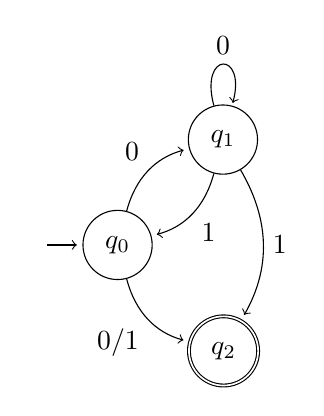
\begin{tikzpicture}[auto, node distance=1cm, shorten >=2pt]
  \node[state,initial,initial text=] (q0) {$q_0$}; 
  \node[state] (q1) [above right=of q0] {$q_1$}; 
  \node[state,accepting] (q2) [below right=of q0] {$q_2$}; 
  \path[->] 
    (q0) edge [bend left] node {0} (q1)
         edge [bend right] node [swap] {0/1} (q2)
    (q1) edge [loop above] node {0} ()
         edge [bend left] node {1} (q0)
         edge [bend left] node {1} (q2);
\end{tikzpicture}

  \caption{A simple example of a NFA}
\end{figure}

To make the $\D$ function \textit{complete}, we can add a \textbf{sink state}, which is just an additional state with no outgoing edges, where all the missing transitions of the other states leads to.

\begin{theorem*}[NFA acceptance]
  A word $w$ is \textbf{accepted} by an NFA $\A$ iff $\hat{\D}\left( q_0, w \right) \cap F \neq \emptyset$, \ie, if at least one of the states when reaching $w$ is a final state.
\end{theorem*}

Like for DFA, we denote by $\L(\A)$ the language accepted by a NFA $\A$, which consists of all and only those words accepted by $\A$.

\begin{theorem*}[NFA equivalence]
  For all NFA $\A$, there exists a DFA $\A'$ \st $\L(\A) = \L(\A')$, and vice versa.
\end{theorem*}

\newpage

\begin{proof*}
  \textit{thesis:} NFA equivalence to DFA.

  \medskip
  Given a NFA $\A = \left(Q,A,\D,q_0,F\right)$, the corresponding DFA is $\A' = \left(Q',A,\d,q_0',F'\right)$ where
  \begin{itemize}
    \item $Q' = 2^Q$
    \item $\forall P \in Q', a \in A \quad \d(P,a) = \D(P,a)$
    \item $q_0' = \{ q_0 \}$
    \item $F' = \{ P \in Q' : P \cap F \neq \emptyset \}$
  \end{itemize}
  and the $P$ is meant for $\A'$ as a state, while for $\A$ as a set of states, \ie, a subset of $Q$.

  \medskip
  We prove by induction on the length of a word $w$ that $\d(q_0',w) = \D(q_0,w)$ holds.
  \begin{itemize}
    \item[\color{pink!200}$\Rightarrow$] \textbf{base case} \quad for $\abs{w} = 0$ it holds that $\d(q_0', \e) = \{q_0\} = \D(q_0,\e)$.

      \textbf{induction step} \quad we assume that the thesis holds for any $\abs{w} \le n$, and we prove it holds for any $wa$, with $a \in A$ (\ie, $\abs{wa} = \abs{w} + 1$).

      By definition, $\d(q_0',wa) = \d\left(\d(q_0',w),a\right)$.
      Then, it holds that $\d(q_0',w) = \D(q_0,w)$ and thus
      \begin{equation*}
        \d(q_0',wa) = \d\left(\D(q_0,w),a\right) = \bigcup_{p \in \D(q_0,w)} \d(\{p\},a) = \bigcup_{p \in \D(q_0,w)} \D(p,a) = \D(q_0,wa)
      \end{equation*}
      By definition, $\A'$ accepts $w$ iff
      \begin{equation*}
        \d(q_0',w) \in F' \quad\iff\quad \D(q_0,w) \in F' \quad\iff\quad \D(q_0,w) \cap F \neq \emptyset
      \end{equation*}
      and thus iff $\A$ accepts $w$.
      Therefore, we can conclude that $\L(\A') = \L(\A)$.
    \item[\color{pink!200}$\Leftarrow$] it's trivial because any DFA it's just a NFA special case, thus every DFA $\A'$ can be equally built as a NFA $\A$.
  \end{itemize}
\end{proof*}

\subsection{\eNFA}

A \eNFA is a NFA with \quoted{$\e$-moves}, \ie, $\e$ is accepted as a possible input by the transition function $\D$.
The definition remains equal, except that the transition function is defined as
\begin{equation*}
  \D: Q \times \tuple{A \cup \set{\e}} \to 2^Q \ .
\end{equation*}

The set of state that can be reached from a given state $q \in Q$ by only applying $\e$-moves, is called $\boldsymbol{\e}$\textbf{-closure} of $q$ ($\e\text{-closure}(q)$).
Moreover, for all $P \in 2^Q$ (\ie, for all subsets of states of $Q$) we define the $\e\text{-closure}(P)=\displaystyle\bigcup_{p \in P} \e\text{-closure}(p)$.

\begin{theorem*}[\eNFA equivalence]
  For all \eNFA $\A$, there exists a NFA $\A'$ \st $\L(\A) = \L(\A')$, and vice versa.
\end{theorem*}

Because DFA recognizes regular languages, also NFA and \eNFA recognize them thanks to the equivalence theorems.

\section{Regular Expressions}

Let $A$ be a finite alphabet, we can have the following regular expression classes:
\begin{itemize}
  \item \textbf{Restricted regular expressions}: built from a finite set of words over $A$ by using the operations union, concatenation and Kleene closure.
  \item \textbf{General regular expressions}: extension of restricted expressions, but also have complementation and intersection operations.
  \item \textbf{Star-free regular expressions}: like the general expressions, but without the Kleene closure.
\end{itemize}
General regular expressions cannot be less expressive than the other two.

\begin{theorem}[FA $\equiv$ RRE]\label{thm:fa_rre}
  For every finite state automaton, there exists a restricted regular expression that defines the same language and vice versa.
\end{theorem}

\begin{proof*}[\nameref{thm:fa_rre}]
  \begin{itemize}
    \item[\color{pink!200}$\Rightarrow$] For this direction, DFA will be used as a choice of automaton.

    Let $\A = \tuple{\set{\vars{q}{1}{n}},A,\d,q_1,F}$ be a DFA.
    Let $R_{i,j}^k$ be the set of words $x$ \st $\d(q_i,x) = q_j$ and for all proper prefixes of $x$, with $y \neq x$ and $y \neq \e$, \ie, all intermediate states, if $\d(q_i,y) = q_l$, then $l \le k$.

    \textbf{base case}
    \begin{equation*}
      R_{i,j}^0 = \begin{cases}
        \{a: \d(q_i,a) = q_j\} \text{, if } i \neq j\\
        \{a: \d(q_i,a) = q_j\} \cup \{\e\} \text{, if } i=j
      \end{cases}
    \end{equation*}

    \textbf{general case}
    \begin{equation*}
      R_{i,j}^k = R_{i,j}^{k-1} \cup \left( R_{i,k}^{k-1} \cdot \left( R_{k,k}^{k-1} \right)^* \cdot R_{k,j}^{k-1} \right)
    \end{equation*}
    \ie, there is a direct edge between $i$ and $j$, or that can be indefinite (that's the meaning of *) intermediate nodes $k$.
  \end{itemize}
\end{proof*}

\newpage

\begin{proof*}[\nameref{thm:fa_rre}]
  \begin{itemize}
    \item[\color{pink!200}$\Leftarrow$] For this proof direction, the automaton used is a \eNFA with at most one final state with no outgoing edges.

    Let $\A$ be a finite alphabet and let $r$ be a RRE over $\A$.

    \textbf{base case}
    \begin{itemize}
      \item if we have $F = \emptyset$, there is no final state that can be reached;
      \item if we have $F = \set{\e}$, we can move only via $\e$-moves, thus a possible scenario is that $q_0$ is also a final state and we stay in $q_0$ with an $\e$-move;
      \item if we have $F = \set{a}$, we can move via $\e$-moves and $a$, but we want to recognize only $a$ thus a possible scenario is that $q_1$ is final and only reachable via an $a$.
    \end{itemize}

    \textbf{inductive step}
    \begin{enumerate}
      \item For the \textit{first} case we consider $r = r_1 \cup r_2$, \ie, the union of two RRE.
        By inductive hypothesis, there exist two \eNFA $\A_1 = (Q_1,A_1,\D_1,q_1,\set{f_1})$ and $\A_2 = (Q_2,A_2,\D_2,q_2,\set{f_2})$, that respectively recognize $\L(r_1)$ and $\L(r_2)$.

        \Wlogt, we assume that $Q_1 \cap Q_2 = \emptyset$.

        Let us define an automaton $\A = \tuple{Q_1 \cup Q_2 \cup \set{q_0,f_0},A,\D,q_0,\set{f_0}}$ \st $\L(\A) = \L(\A_1) \cup \L(\A_2)$, where
        \begin{itemize}
          \item $\D(q_0, \e) = \set{q_1,q_2}$;
          \item $\D(q, a) = \D_1(q,a) \fort q \in Q_1 \setminus \set{f_1} \andt a \in A \cup \set{\e}$;
          \item $\D(q, a) = \D_2(q,a) \fort q \in Q_2 \setminus \set{f_2} \andt a \in A \cup \set{\e}$;
          \item $\D(f_1,\e) \ = \ \set{f_0} \ = \ \D(f_2,\e)$.
        \end{itemize}

      \item As a \textit{second} case we consider $r = r_1 \cdot r_2$, \ie, the concatenation of two RRE, with $\A_1 \andt \A_2$ described as in the first case.
        Here, an automaton $\A$ for $\L(r_1 \cdot r_2)$ is $\tuple{Q_1 \cup Q_2,A,\D,q_1,\set{f_2}}$, where
        \begin{itemize}
          \item $\D(q, a) = \D_1(q,a) \fort q \in Q_1 \setminus \set{f_1} \andt a \in A \cup \set{\e}$;
          \item $\D(q, a) = \D_2(q,a) \fort q \in Q_2 \andt a \in A \cup \set{\e}$;
          \item $\D(f_1,\e) = \set{q_2}$.
        \end{itemize}
      \item The \textit{third} and final case is when $r = r_1^*$.
        By hypothesis there exists an automaton $\A_1 = (Q_1,A_1,\D_1,q_1,\set{f_1})$ that recognizes $\L(\A_1)$.
        Therefore, an automaton for $r$ is $\A = \tuple{Q_1 \cup \set{q_0,f_0},A,\D,q_0,\set{f_0}}$, where
        \begin{itemize}
          \item $\D(q_0, \e) = \set{q_1,f_0}$;
          \item $\D(q, a) = \D_1(q,a) \fort q \in Q_1 \setminus \set{f_1} \andt a \in A \cup \set{\e}$;
          \item $\D(f_1,\e) = \set{q_1,f_0}$.
        \end{itemize}
    \end{enumerate}
  \end{itemize}
\end{proof*}

It follows that RRE define regular languages.

\begin{theorem*}[Closure properties]
  Regular languages are closed under Boolean operations (union $\cup$, intersection $\cap$, complementation $\neg$), concatenation (\cdot) and Kleene closure (*).
\end{theorem*}

The construction of the automaton that recognizes the languages obtained by means of these operations is \textbf{effective}, \ie, not only we can claim that there exists an automaton, but we can also build it.

\begin{corollary*}
  Restricted regular expressions are as expressive as general regular expressions.
\end{corollary*}

\begin{theorem*}[Automaton decidability]
  Given two automata $\A$ and $\A'$, the problems of establishing whether
  \begin{itemize}
    \item $\L(\A) \neq \emptyset$ \hspace{41pt} (\textit{emptiness})
    \item $\L(\A) = A^*$ \hspace{38pt} (\textit{universality})
    \item $\L(\A) \subseteq \L(\A')$ \hspace{20pt} (\textit{model-checking/inclusion})
    \item $\L(\A) = \L(\A')$ \hspace{20pt} (\textit{equivalence})
  \end{itemize}
  are \textbf{decidable}.
\end{theorem*}

\subsection{Equivalency}

\begin{definition}[Word equivalence]\label{def:word_eq}
  Fixed a finite automaton DFA $\A$, the equivalence of words, denoted with $\approx_{\A}$, is
  \begin{equation*}
    u \approx_{\A} v \ \iff \ \d\left( q_0,u \right) = \d\left( q_0,v \right)
  \end{equation*}
  \ie, they reach the same state.
\end{definition}

\begin{example*}
  \begin{center}
    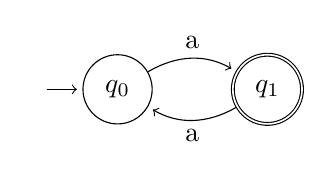
\begin{tikzpicture}[auto, node distance=1cm, shorten >=2pt]
  \node[state,initial,initial text=] (q0) {$q_0$}; 
  \node[state,accepting] (q1) [right=of q0] {$q_1$}; 
  \path[->] 
    (q0) edge [bend left] node {a} (q1)
    (q1) edge [bend left] node {a} (q0);
\end{tikzpicture}

  \end{center}
  Given the above automaton, we have that:
  \begin{itemize}
    \item if $u = aaa$ and $v = aa$, then $u \not\approx_{\A} v$
    \item if $u = aaa$ and $v = aaaaa$, then $u \approx_{\A} v$
  \end{itemize}
\end{example*}

The word equivalence has also the following properties:
\begin{itemize}
  \item $\approx_{\A}$ has always a \textbf{finite index} (\ie, finitely many classes), in particular $\text{idx}(\approx_{\A}) \le \abs{Q}$, because we have at most one class for each state;
  \item $\approx_{\A}$ is a \textbf{right congruence}, or \textbf{right invariant equivalence}, if given two words $u,v$ \st $u \approx_{\A} v$, for all words $w$ it holds that $uw \approx_{\A} vw$;
  \item $\approx_{\A}$ \textbf{partitions} $\L(\A)$, which formally means that if $u \approx_{\A} v$ then $u \in L \iff v \in L$. This can be rephrased as: $\L(\A)$ is a finite union of equivalence classes.
\end{itemize}

\begin{proof*}[Right congruence]
  By definition, if $u \approx_{\A} v$ then $\d(q_0,u) = \d(q_0,v)$.
  Following the hypothesis we have that
  \begin{align*}
    \forall w \quad \d(q_0,uw) &= \d(\d(q_0,u),w)\\
    &= \d(\d(q_0,v),w)\\
    &= \d(q_0,vw)
  \end{align*}
  therefore $\forall w \quad uw \approx_{\A} vw$.
\end{proof*}

\begin{definition*}[Language equivalence]
  Fixed an arbitrary language $L \subseteq \S^*$ ($L$ doesn't need to be regular), we have $u \approx_{L} v$ if
  \begin{equation*}
    \forall w \in \S^* \quad uw \in L \iff vw \in L
  \end{equation*}
  holds.
\end{definition*}

The language equivalence has also the same word equivalence properties with the difference that can be infinite:
\begin{itemize}
  \item $\approx_{L}$ may have \textbf{finite} or \textbf{infinite} indexes depending on $L$;
  \item $\approx_{L}$ is a \textbf{right congruence}/\textbf{invariance};
  \item $\approx_{L}$ \textbf{partitions} $L$.
\end{itemize}

\begin{lemma*}[Refinement lemma]
  Given a language $L$ and an equivalence $\approx$, which is a right congruence and partitions $L$, then $\approx$ is a refinement of $\approx_L$, because if $u \approx v$ then $u \approx_L v$.

  \medskip
  In other words, $\approx_L$ is the \textbf{coarsest}\footnote{least number of classes} right congruence that partitions $L$.
\end{lemma*}

\begin{theorem}[Myhill-Nerode]\label{thm:myhill_nerode}
  Fixed a language $L \subseteq \S^*$, the following conditions are equivalent:
  \begin{enumerate}
    \item $L$ is regular;
    \item $L$ is partitioned by some right congruence of finite index;
    \item $\approx_L$ has finite index.
  \end{enumerate}
\end{theorem}

A way to remember this theorem is that $L$ is regular iff $\approx_L$ has finite index.

\newpage

\begin{proof*}[\nameref{thm:myhill_nerode}]
  \begin{itemize}
    \item[\color{pink!200}$1 \Rightarrow 2$] We assume that $L$ is regular and we want to find some right congruence of finite index that partitions $L$.

      If $L$ is regular it means that there is a DFA $\A$ that recognizes it ($\L(\A) = L$).
      Moreover, by definition of \nameref{def:word_eq} $\approx_{\A}$ and its properties, we have that is a right congruence with finite index that partitions $L$.
    \item[\color{pink!200}$2 \Rightarrow 3$] By hypothesis we assume that there exists some right congruence $\approx$ of finite index that partitions $L$.

      Due to the refinement lemma, if $\approx$ is a right congruence that partitions $L$, and this is granted by hypothesis, then $\approx$ is a refinement of $\approx_L$.
      Being a refinement we have that $\text{idx}(\approx) \ge \text{idx}(\approx_L)$ and because $\approx$ is finite, then $\approx_L$ must be finite too.
    \item[\color{pink!200}$3 \Rightarrow 1$] We assume that $\approx_L$ has finite index and we want to prove that $L$ is regular.

      We construct an automaton $\A_L = \tuple{\S, Q, \d, q_0, F}$ where
      \begin{itemize}
        \item $Q = \set{[u]_{\approx_L} \mid u \in \S^*}$
        \item $q_0 = [\e]_{\approx_L}$
        \item $F = \set{[u]_{\approx_L} \mid u \in L}$
        \item $\d(q,a) = q'$
      \end{itemize}
      with the $\d$ function well-defined because:
      \begin{itemize}
        \item given a word $u$, we will have $q = [u]_{\approx_L}$ and $q = [ua]_{\approx_L}$
        \item given a word $v$, we will have $q = [v]_{\approx_L}$ and $q = [va]_{\approx_L}$
      \end{itemize}
      thus $\approx_L$ is a right congruence.

      For this reason, we have also that $\L(\A_L) = L$, so $\A_L$ recognizes the language $L$, which implies that $L$ is regular.
  \end{itemize}
\end{proof*}

\bigskip
So far our automata and regular expressions describe \emph{finite} words. But the systems we ultimately want to verify -- operating systems, controllers, network protocols -- are \textbf{reactive}: they are not meant to terminate, they run indefinitely while interacting with their environment, so their behavior is naturally an \emph{infinite} sequence of states. To reason about them we must lift the whole machinery just developed -- automata, closure properties, decision problems -- from finite words to infinite ones. That is the subject of the next chapter.

\chapter{Automata on Infinite Words}\label{cha:automata}

Reactive systems never stop, so their computations are infinite words ($\w$-words), which have no last symbol on which to test acceptance. \Buchi's insight was disarmingly simple: instead of asking to \emph{end} in a final state, ask to \emph{visit} a final state \emph{infinitely often} -- a condition on the set $\inf{\s}$ of states seen infinitely many times. This single change generates the rich theory of this chapter (\Buchi, Muller and Rabin automata; closure; complementation; determinisation; star-free languages). The chapter then turns the theory back onto the systems themselves, modelling reactive programs as Fair Transition Systems, whose fairness conditions are nothing but constraints on $\inf{\s}$.

\section{\Buchi automata}

Given an alphabet $A$ and set of finite words $W \subseteq A^*$:
\begin{itemize}
  \item \textbf{\wword}: is an infinite concatenation of symbols, \ie, $a_0 a_1 \ldots$;
  \item \textbf{Kleene closure} $W^*$: is the set of finite concatenations of words from $W$;
  \item \textbf{\wclo} $W^\w$: is the set of infinite concatenations of words from $W$, \ie, $W^\w = \set{ \a \in \Aw : \a = w_0 w_1 \ldots}$;
  \item \textbf{vectorial closure} $\overrightarrow{W}$: is the set of infinite words that have infinitely-many finite prefixes in $W$, \ie, $\overrightarrow{W} = \set{\a \in \Aw : \exists^\w n \ \a (0,n) \in W}$;
  \item \textbf{infinite} of a word $\inf{\a}$: is the set of symbols which occur infinitely many times in an infinite word $\a$, \ie, $\inf{\a} = \set{ a \in A : \exists^\w n \ \, \a(n) = a},\ \forall \a \in \Aw$.
\end{itemize}

\begin{note}
  The operator $\text{Inf}$ will be applied to two different kinds of object, and it pays to keep them apart. Applied to an input \wword $\a$, the set $\inf{\a} \subseteq A$ collects the \emph{symbols} occurring infinitely often. Applied to a computation $\s$ of an automaton (a sequence of \emph{states}), the set $\infs \subseteq Q$ collects the \emph{states} visited infinitely often. The \Buchi acceptance condition below uses the latter, $\infs \cap F \neq \emptyset$.
\end{note}

\begin{note}
  When dealing with $W^\w$ we assume that $\e \notin W$, otherwise the set can degenerate creating finite words, \eg, $u \e \e \dots$
\end{note}

\begin{definition*}[\Buchi automaton]
  A \Buchi automaton is a tuple $\A = \NBA$ where all components are defined as in the case of NFA (in particular $\D \subseteq Q \times A \times Q$).
\end{definition*}

The difference between a \Buchi automaton and an NFA stands in the mechanism of checking if a word belongs or not in a language.
Recall that for finite state automata, this is done by reading the entire word and check if we ended in a finite state or not.
Of course, this approach is not applicable to infinite-length words and \Buchi automata fill this gap.

\begin{definition*}[\Buchi computation]
  A computation $\s$ of $\A$ on an \wword $\a$ is \st
  \begin{itemize}
    \item $\s(0) = q_0$, \ie, must start from $q_0$;
    \item $\forall i \ge 0 \quad \Big( \s(i), \a(i), \s'(i+1) \Big) \in \D$, \ie, for all the other steps there exists a transition in $\A$;
  \end{itemize}
  and we call the computation \textbf{successful} if $\infs \cap F \neq \emptyset$, \ie, during the computation we go through at least one final state.

  \bigskip
  We say that a \Buchi automaton $\A$ \textbf{accepts} an \wword $\a$ iff there exists a successful computation of $\A$ on $\a$.
  Moreover, the language $\L(\A)$ recognized by $\A$ is the set of all and only those \wwords accepted by $\A$.

  \bigskip
  An \wlan $L \subseteq \Aw$ is \wreg iff there exists a \Buchi automaton that recognizes it, or equally, exists $\A$ for which it holds that $\L(\A) = L$.
\end{definition*}

\begin{note}
  It's specified ``A'' computation instead of ``The'' because we have infinite-many possible computations.
\end{note}

\begin{example*}
  Given $A = \set{a, b, c}$ find a language $L$ \st between any two consecutive occurrences of the symbol $a$ there is an even number of occurrences of the symbols $b$ and $c$.
  \begin{center}
    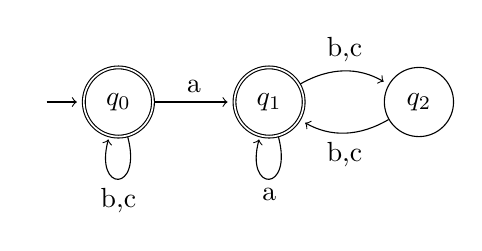
\begin{tikzpicture}[auto, node distance=1cm, shorten >=2pt]
  \node[state,initial,initial text=,accepting] (q0) {$q_0$}; 
  \node[state,accepting] (q1) [right=of q0] {$q_1$}; 
  \node[state] (q2) [right=of q1] {$q_2$}; 
  \path[->] 
    (q0) edge [loop below] node {b,c} ()
         edge node {a} (q1)
    (q1) edge [loop below] node {a} ()
         edge [bend left] node {b,c} (q2)
    (q2) edge [bend left] node {b,c} (q1);
\end{tikzpicture}

  \end{center}
  or equally
  \begin{center}
    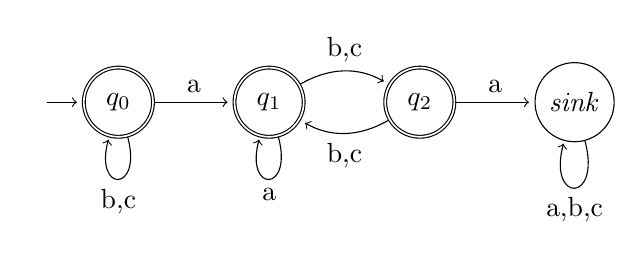
\begin{tikzpicture}[auto, node distance=1cm, shorten >=2pt]
  \node[state,initial,initial text=,accepting] (q0) {$q_0$}; 
  \node[state,accepting] (q1) [right=of q0] {$q_1$}; 
  \node[state,accepting] (q2) [right=of q1] {$q_2$}; 
  \node[state] (sink) [right=of q2] {\textit{sink}}; 
  \path[->] 
    (q0) edge [loop below] node {b,c} ()
         edge node {a} (q1)
    (q1) edge [loop below] node {a} ()
         edge [bend left] node {b,c} (q2)
    (q2) edge [bend left] node {b,c} (q1)
         edge node {a} (sink)
    (sink) edge [loop below] node {a,b,c} ();
\end{tikzpicture}

  \end{center}
  because, working over infinite words, it means that the computation doesn't stop, therefore $q_2$ can be final because we know that it will come back to $q_1$ if the word is accepted.
\end{example*}

\begin{theorem*}[Closure properties]
  \begin{enumerate}
    \item If $V \subseteq A^*$ is regular, then $V^\w$ is \wreg.
    \item If $V \subseteq A^*$ is regular and $L \subseteq \Aw$ is \wreg, then $V \cdot L$ is \wreg.
    \item If $L_1, L_2$ are \wreg, then both $L_1 \cup L_2$ and $L_1 \cap L_2$ are \wreg.
  \end{enumerate}
\end{theorem*}

\begin{proof*}[Closure property 1]
  Let $\A = \NBA$ be an NFA that recognizes $V$.
  Since $V^\w = \tuple{V \setminus \set{\e}}^\w$, we assume that $\e \notin V$.
  We split the proof in two cases, and as first we consider the one where there are no transitions entering in $q_0$.

  \bigskip
  A \Buchi automaton $\A'$ that recognizes $V^\w$ can be obtained from $\A$ by replacing all the transitions that go to a final state, \ie, $\tuple{s, a, s'} \in \D$ with $s' \in F$, with transitions that consume the same symbol but returns to the initial state $q_0$, \ie, $\tuple{s, a, q_0}$, and marking $q_0$ as the only final state.
  \begin{displaybox}
    \begin{minipage}{0.5\textwidth}
      \begin{center}
        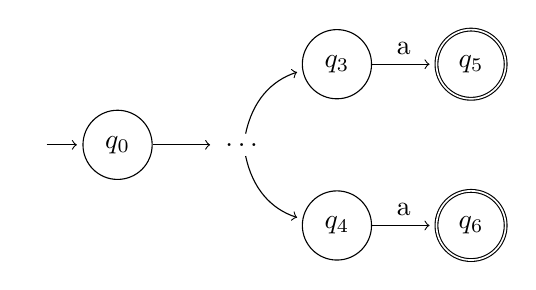
\begin{tikzpicture}[auto, node distance=0.8cm, shorten >=2pt]
  \node[state,initial,initial text=] (q0) {$q_0$}; 
  \node (d) [right=of q0] {$\dots$}; 
  \node[state] (q3) [above right=of d] {$q_3$}; 
  \node[state] (q4) [below right=of d] {$q_4$}; 
  \node[state,accepting] (q5) [right=of q3] {$q_5$}; 
  \node[state,accepting] (q6) [right=of q4] {$q_6$}; 
  \path[->] 
    (q0) edge (d)
    (d) edge [bend left] (q3)
    (d) edge [bend right] (q4)
    (q3) edge node {a} (q5)
    (q4) edge node {a} (q6);
\end{tikzpicture}

      \end{center}
    \end{minipage}
    \begin{minipage}{0.05\textwidth}
      \begin{center}
        $\Rightarrow$
      \end{center}
    \end{minipage}
    \begin{minipage}{0.4\textwidth}
      \begin{center}
        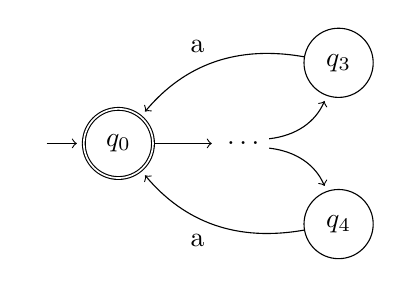
\begin{tikzpicture}[auto, node distance=0.8cm, shorten >=2pt]
  \node[state,initial,initial text=,accepting] (q0) {$q_0$}; 
  \node (d) [right=of q0] {$\dots$}; 
  \node[state] (q3) [above right=of d] {$q_3$}; 
  \node[state] (q4) [below right=of d] {$q_4$}; 
  \path[->] 
    (q0) edge (d)
    (d) edge [bend right] (q3)
    (d) edge [bend left] (q4)
    (q3) edge [bend right] node [swap] {a} (q0)
    (q4) edge [bend left] node {a} (q0);
\end{tikzpicture}

      \end{center}
    \end{minipage}
  \end{displaybox}

  However, in the case that the initial state $q_0$ has entering transitions, we can make this case equivalent to the previous by adding a new state $q_0'$, which will be our new initial state, and then add the same outgoing edges that has $q_0$ to $q_0'$.
  \begin{displaybox}
    \begin{minipage}{0.4\textwidth}
      \begin{center}
        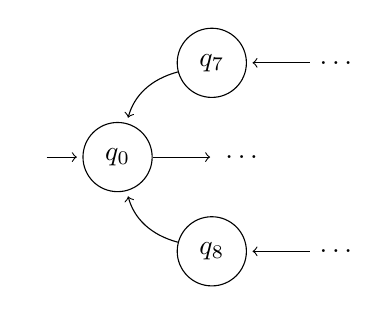
\begin{tikzpicture}[auto, node distance=0.8cm, shorten >=2pt]
  \node[state,initial,initial text=] (q0) {$q_0$}; 
  \node[state] (q7) [above right=of q0] {$q_7$}; 
  \node[state] (q8) [below right=of q0] {$q_8$}; 
  \node (d1) [right=of q7] {$\dots$}; 
  \node (d2) [right=of q8] {$\dots$}; 
  \node (d3) [right=of q0] {$\dots$}; 
  \path[->] 
    (q7) edge [bend right] (q0)
    (q8) edge [bend left] (q0)
    (q0) edge (d3)
    (d1) edge (q7)
    (d2) edge (q8);
\end{tikzpicture}

      \end{center}
    \end{minipage}
    \begin{minipage}{0.05\textwidth}
      \begin{center}
        $\implies$
      \end{center}
    \end{minipage}
    \begin{minipage}{0.5\textwidth}
      \begin{center}
        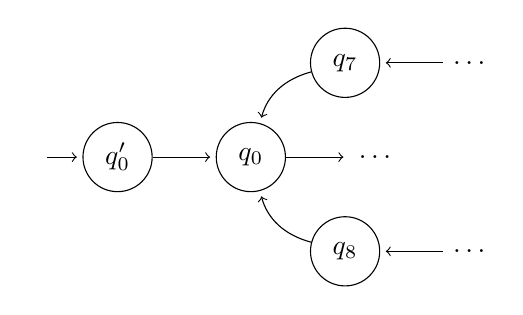
\begin{tikzpicture}[auto, node distance=0.8cm, shorten >=2pt]
  \node[state] (q0) {$q_0$}; 
  \node[state] (q7) [above right=of q0] {$q_7$}; 
  \node[state] (q8) [below right=of q0] {$q_8$}; 
  \node (d1) [right=of q7] {$\dots$}; 
  \node (d2) [right=of q8] {$\dots$}; 
  \node (d3) [right=of q0] {$\dots$}; 
  \node[state,initial,initial text=] (q0p) [left= of q0] {$q_0'$}; 
  \path[->] 
    (q7) edge [bend right] (q0)
    (q8) edge [bend left] (q0)
    (q0) edge (d3)
    (d1) edge (q7)
    (d2) edge (q8)
    (q0p) edge (q0);
\end{tikzpicture}

      \end{center}
    \end{minipage}
  \end{displaybox}
\end{proof*}

\begin{proof*}[Closure property 2]
  Prove it by yourself
\end{proof*}

\begin{proof*}[Closure property 3]
  Prove it by yourself
\end{proof*}

\begin{definition*}[\wreg expression]
  An \wreg expression has the form
  \begin{equation*}
    \bigcup_{i=1}^n U_i \cdot V_i^\w
  \end{equation*}
  where $U_i, V_i$ are regular expressions for all $i$.
\end{definition*}
Let $\A = \NBA$ be a BA\footnote{\Buchi Automaton}, and take a finite word $w \in A^*$ and two states $s, s'$ from $Q$.
We denote by $s \to_w s'$ to mean a computation of $\A$ on $w$ that leads from $s$ to $s'$.

For each pair of states $s, s' \in Q$, we define the language $W_{s,s'} = \set{w \in A^* : s \to_w s'}$, which is also regular for all $s, s' \in Q$.
To prove that is regular, we can define an automaton $\A$ that recognizes $W_{s,s'}$ like so
\begin{equation*}
  \A_{W_{s,s'}} = \tuple{Q, A, \D, s, \set{ s'}}
\end{equation*}

\begin{theorem*}
  For any BA $\A$ there exists an \wreg expression $r$ that defines the same language, and vice versa.
\end{theorem*}

\begin{proof*}
  \begin{itemize}
    \item[\color{pink!200}$\Leftarrow$] Because $r$ is an \wreg expression, it means that
    \begin{equation*}
      r = \bigcup_{i=1}^n U_i \cdot V_i^\w
    \end{equation*}
    We can exploit the closure properties like so
    \begin{itemize}
      \item the exponentiation $V_i^\w$ is \wreg for closure 1 ($\w$ exponentiation)
      \item the concatenation $U_i \cdot V_i^\w$ is regular for closure 2 (concatenation)
      \item the union $\bigcup_{i=1}^n U_i \cdot V_i^\w$ is regular for closure 3 (union)
    \end{itemize}
    and say that $r$ is regular, thus it defines a language.

    \item[\color{pink!200}$\Rightarrow$] Let $\A = \NBA$ be a BA.
      Checking whether there exists at least one word which is a set by a \Buchi automaton, given the \Buchi automaton, is a simple reachability problem, because we only need to know whether we're able to reach a final state starting from the initial state $q_0$ and then check for a loop over that final state.
      \begin{center}
        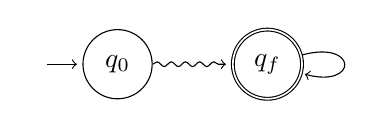
\begin{tikzpicture}[auto, node distance=1cm, shorten >=2pt, decoration={snake,segment length=1.8mm,amplitude=0.3mm,post length=4pt}]
  \node[state,initial,initial text=] (q0) {$q_0$}; 
  \node[state,accepting] (qf) [right=of q0] {$q_f$}; 
  \draw[->, decorate] (q0) -- (qf);
  \path[->] (qf) edge [loop right] (qf);
\end{tikzpicture}

      \end{center}
      We can express this set with
      \begin{equation*}
        \bigcup_{q_f \in F} W_{q_0,q_f} \cdot \left( W_{q_f,q_f} \right)^\w
      \end{equation*}
      \ie, the union for all possible finite states $q_f$ of the set of computations that lead from $q_0$ to $q_f$ and which can cycle infinitely on $q_f$.
  \end{itemize}
\end{proof*}

\begin{definition*}
  An \wword $\a \in \Aw$ is called \textbf{ultimately periodic} if $\a = u \cdot v^\w$, with $u,v \in A^*$.
\end{definition*}

Ultimately periodic words are infinite, but, thanks to their structure, can be finitely represented.

\begin{corollary*}
  Every non-empty \wreg language $L$ includes an ultimately periodic $\w$-word.
\end{corollary*}

\begin{proof*}[corollary]
  Because we can represent a language $L$ as
  \begin{equation*}
    L = \bigcup_{i=1}^n U_i \cdot V_i^\w,
  \end{equation*}
  then, if $L \neq \emptyset$, there exists $i$ \st $U_i \cdot V_i^\w \neq \emptyset$ that is, there exists $\a \in U_i \cdot V_i^\w$.

  Therefore, $\a$ can be represented as
  \begin{equation*}
    \a = u v_0 v_1 v_2 \ldots
  \end{equation*}
  where each $v_i$ belongs to $V$.

  It immediately follows that also $\a' = u v_0 v_0 v_0 \ldots = u \cdot v^\w$ belongs to $L$.
\end{proof*}

\begin{theorem*}
  The emptiness problem for BA is \textbf{decidable}.
\end{theorem*}

\begin{proof*}
  If the language isn't empty, it contains an ultimately periodic $\w$-word.
  Checking this condition can be done by solving a simple reachability problem.
\end{proof*}

\begin{example*}[\wlan which isn't \wreg]
  Let $\beta$ be a non-ultimately periodic \wword and let $\L(\b)$ be the language of those \wwords in $\Aw$ which have a common suffix with $\beta$.

  We can conclude that $\L(\b)$ is not empty because for sure we will have that $\b\in \L(\b)$.
  Furthermore, all words in $\L(\b)$ are non-ultimately periodic as, by definition, have a suffix in common with $\b$ and $\b$ itself is non-ultimately periodic.
  However, a language that doesn't include any ultimately periodic word is not \wreg, thus $\L(\b)$ is non \wreg.

  \bigskip
  This example shows also that there exist non-ultimately periodic languages which are non-empty.
\end{example*}

\subsection{Complementation}

\begin{definition*}[Congruence]
  An equivalence relation $\sim$ over a set $A$ is a \textbf{congruence} (with respect to concatenation) if
  \begin{equation*}
    \forall x, x', y, y' \in A \qquad x \sim y \land x' \sim y' \;\implies\; xx' \sim yy'\; .
  \end{equation*}
\end{definition*}

\begin{example*}[Congruence over $A^*$ (\emph{parity})]
  Two words $u,v \in A^*$ belong to the same class if they have the same parity, \ie, both of them have either an even or odd number of symbols.
\end{example*}

Equivalence of finite index means ``with a finite number of classes''.

\begin{definition}[Saturation]\label{def:saturation}
  A congruence $\sim$ \textbf{saturates} an \wlan $L \subseteq \Aw$ if, for all pairs of $\sim$-classes $U \andt V$, we have that
  \begin{equation*}
    U V^\w \cap L \neq \emptyset \quad \implies \quad U V^\w \subseteq L
  \end{equation*}
  \ie, if there exist at least an \wword with the pattern $U V^\w$, then all the words of that form belong to the language $L$.

  \bigskip
  Moreover, let $\sim$ be a congruence and $L \subseteq \Aw$; if $\sim$ saturates $L$, then $\sim$ saturates also $\ol{L}$.
\end{definition}

\begin{proof*}[\nameref{def:saturation}]
  By contradiction, let us assume $\sim$ doesn't saturate $\ol{L}$.
  This implies that there exists $U, V$ $\sim$-classes \st $U V^\w \cap \ol{L} \neq \emptyset$, but $U V^\w \nsubseteq \ol{L}$.
  Hence, there exists $\a \in U V^\w$ \st $\a \in L$.

  By hypothesis, since $\sim$ saturates $L$, by definition we have that $U V^\w \cap L \neq \emptyset$ which follows that $U V^\w \subseteq L$, and this is a contradiction.
\end{proof*}

The saturation property partitions words of the pattern $U V^\w$ into classes of the congruence.

\bigskip
Let $\A = \NBA$ with $w \in A^*$ and $s, s' \in Q$.
We write $s \to_w^F s'$ if there exists a computation of $\A$ on $w$ from $s$ to $s'$, where at least one state of the computation (including $s$ and $s'$) is a final state.
The set is denoted with
\begin{equation*}
  W_{s,s'}^F = \set{w \in A^* : s \to_w^F s'}
\end{equation*}

\begin{exercise*}
  Show that $W_{s,s'}^F$ is regular.
\end{exercise*}

Now we generalize $\sim_{\A}$ to the relation $\approx_{\A}$.

\begin{definition*}[Relation $\approx_{\A}$]
  Let $\A = \NBA$ be a BA.
  We define a relation $\approx_{\A}$ on $A^*$ \st $u \approx_{\A} v$ if for all pairs of state $s, s' \in Q$
  \begin{equation*}
    s \to_u s' \iff s \to_v s' \quad \andt \quad s \to_u^F s' \iff s \to_v^F s'
  \end{equation*}
  and vice versa.

  \bigskip
  Moreover, given a BA $\A$, the relation $\approx_{\A}$ is a congruence of a finite index that saturates $\L(\A)$.
\end{definition*}

\begin{proof*}
  Let $\A = \NBA$ and $U,V$ classes of $\approx_{\A}$.
  Let us consider an \wword $\a \in UV^\w \cap \L(\A)$, to prove that if a single word belongs to $\L(\A)$, then all the others belongs too.

  Given this hypothesis, it means that there exists a successful computation of $\A$ on $\a$.
  Moreover, from $\a \in UV^\w$ it follows that there exists $u \in U$ and $v_1, v_2, v_3, \ldots \in V$ \st $\a = u v_1 v_2 v_3 \ldots$ .
  From the successful computation we can extract an infinite subsequence of states $q_0, s_1, s_2, \ldots$ \st we can go from $q_0$ to $s_1$ by reading $u$, then to $s_2$ by reading $v_1$ and so fort, \ie,
  \begin{equation*}
    q_0 \to_u s_1 \to_{v_1} s_2 \to_{v_2} s_3 \ldots
  \end{equation*}
  which we can generalize with
  \begin{equation*}
    s_i \to_{v_i}^F s_{i+1} \; .
  \end{equation*}

  Notice the $F$, which is there because the computation is successful, \ie, we pass through a final state infinitely many times.

  \bigskip
  Now we consider another \wword $\b \in UV^\w$, to prove that $\b \in \L(\A)$.
  Since $\b \in UV^\w$, it can be written as $u' v_1' v_2' \ldots$.
  Now, because $u \approx_{\A} u' \andt v_i \approx_{\A} v_i' \forall i$, it holds that
  \begin{equation*}
    q_0 \to_{u'} s_1 \to_{v_1'} s_2 \to_{v_2'} s_3 \ldots
  \end{equation*}
  and in general
  \begin{equation*}
    s_i \to_{v_i'}^F s_{i+1}
  \end{equation*}
  for an infinite number of indexes $i$.

  We can conclude that there exists a successful computation of $\A$ on $\b$, thus $\b \in \L(\A)$.
\end{proof*}

\begin{lemma*}
  Let $\sim$ be a congruence of finite index on $A^*$.
  For all \wwords $\a \in \Aw$, there exists two classes $U \andt V$ of $\sim$ \st
  \begin{equation*}
    \a \in UV^\w
  \end{equation*}
  with $V \cdot V \subseteq V$.
\end{lemma*}

This means that if we have a congruence of finite index, any \wword can be written as a finite prefix (word from $U$) followed by an infinite sequence of finite words (belonging to $V$).

From this lemma it follows that, given an \wlan $L \subseteq \Aw$ and a congruence of finite index $\sim$ that saturates $L$, it holds that
\begin{equation*}
  L = \bigcup_{i=1}^n U_i V_i^\w
\end{equation*}
where $U \andt V$ are $\sim$-classes \st $UV^\w \cap L \neq \emptyset$.

\begin{proof*}
  \begin{itemize}
    \item[\color{pink!200}$\Rightarrow$] We're going to prove that $L \subseteq \bigcup_{i=1}^n U_i V_i^\w$.

      To prove it, we can exploit the previous lemma, to say that we can take any \wword $\a \in L$ and write it as $UV^\w$.
      Then, by collecting all the \wwords in $L$ and because the relation of finite index, it means that we have a finite number of $UV^\w$ \st each one represents at least an \wword of $L$, which mathematically it's the following set
      \begin{equation*}
        \bigcup_{i=1}^n U_i V_i^\w
      \end{equation*}

    \item[\color{pink!200}$\Leftarrow$] We're going to prove that $L \supseteq \bigcup_{i=1}^n U_i V_i^\w$.

      Recalling previous theorem about saturation of $\sim$, we can say that since $\sim$ saturates $L$, if we have that $UV^\w \cap L \neq \emptyset$, then all the elements of $UV^\w$ must be in $L$, therefore $UV^\w \subseteq L$.
      This proves that $\bigcup_{i=1}^n U_i V_i^\w \subseteq L$.
  \end{itemize}
\end{proof*}

\begin{theorem}[Closure under complementation of \wreg languages]\label{thm:comp_closure}
  If $L \subseteq \Aw$ is an \wreg language, then $\ol{L} = \Aw - L$ is \wreg as well.
  Moreover, from a BA for $L$ we can build a BA for $\ol{L}$.
\end{theorem}

\begin{proof*}[\nameref{thm:comp_closure}]
  Let $\A$ be a BA \st $\L(\A) = L$.
  We already proved that $\approx_{\A}$ is a congruence of finite index that saturates $\ol{L}$.
  By the previous corollary, it follows that we can describe the complement of $L$ as $\bigcup_{i=1}^n U_i V_i^\w$, where $U_i,V_i$ are $\approx_{\A}$ classes \st $U_i V_i^\w \cap \ol{L} \neq \emptyset$ for all $i$.

  Since $U_i, V_i$ are \wreg languages for each $i$, by closure of \wreg languages under \wclo, concatenation and union, we can conclude that $\ol{L}$ is an \wreg language.
\end{proof*}

Let us show that the construction of the BA for $\ol{L}$ is \textbf{effective}.

First we have to find the classes $U \andt V$ that contribute to automaton for $\ol{L}$, \ie, which satisfy the following property
\begin{equation*}
  UV^\w \cap \ol{L} \neq \emptyset \quad \iff \quad UV^\w \cap L = \emptyset
\end{equation*}
because $\approx_{\A}$ saturates $L$.

We recall that the construction of a BA for $UV^\w \cap L$ is effective and the emptiness checking is decidable and easily solvable.
Thus, since BA are closed under union, we can build an automaton for $\ol{L}$ in the same way, \ie, with the same properties.

\bigskip
Given two BA $\A \andt \A'$, the following problems are \textbf{decidable}:
\begin{itemize}
  \item \emph{universality} problem: $\L(\A) = \Aw$, which is decidable because we can check if the complement language is empty (emptiness problem for complement);
  \item \emph{model-checking} problem: $\L(\A) \subseteq \L(\A')$, and it's decidable because $\L(\A) \cap \ol{\L(\A')} = \emptyset$, thus if the first is true, also the second it's true, and vice versa;
  \item \emph{equivalence} problem: $\L(\A) = \L(\A')$, and it's decidable because it's equal to $\L(\A) \subseteq \L(\A') \andt \L(\A) \supseteq \L(\A')$, thus we can reduce both to the previous problem.
\end{itemize}

\begin{theorem}[\wreg languages characterization]\label{thm:wreg_lang_char}
  Every \wreg language is \textit{uniquely} characterized by the set of its ultimately periodic \wwords.
\end{theorem}

In other words, this theorem means that if we know the set of ultimately periodic words belonging to a given automaton, we're able to identify this automaton, \ie, if two automata have the exactly equal set of ultimately periodic words, then they represent the same language.

\begin{proof*}[\nameref{thm:wreg_lang_char}]
  Let us denote the set of ultimately periodic \wwords of a language $L$ with $\text{UP}(L)$.
  Given two languages $L_1 \andt L_2$, if we have that $\text{UP}(L_1) = \text{UP}(L_2)$ and $L_1,L_2$ are \wreg languages, then $L_1 = L_2$. The opposite it's trivially true, because if they're equal, it's obvious that the ultimately periodic \wwords are the same.

  \bigskip
  For hypothesis, suppose that if $\text{UP}(L_1) = \text{UP}(L_2)$, then $L_1 \neq L_2$.

  \Wlogt, let us assume that $L_1 - L_2 = L$ (or vice versa) with $L \neq \emptyset$.
  Since
  \begin{equation*}
    L = L_1 - L_2 = L_1 \cap \ol{L_2} \neq \emptyset
  \end{equation*}
  from the closure properties of \wreg languages, it follows that $L, L_1 \andt L_2$ are \wreg languages.
  Moreover, because $L$ is not empty, there must be at least an ultimately periodic \wword belonging to it.
  This is a contradiction, because our hypothesis was that the sets of ultimately periodic words of $L_1 \andt L_2$ were the same, therefore their difference must not contain any ultimately periodic \wword.
\end{proof*}

\subsection{Determinization problem}

Determinization means that we want to understand whether there exists a class of automata that is as expressive as \Buchi automata, but it's deterministic.
That's because, the complementation of this class should be easy and solvable in the same way as done with finite automata.

The first natural candidates would be deterministic \Buchi automata, but as we will see, they're not as expressive as non-deterministic BA, thus they don't fit into the determinization problem class.

\begin{definition*}[Deterministic \Buchi Automata (DBA)]
  A DBA is a tuple $\DBA$ where $Q,A,q_0,F$  are defined as for BA, while $\d: Q \times A \to Q$.

  The computation $\s$ of $\A$ on an \wword $\a$ is successful if $\infs \cap F \neq \emptyset$.

  Acceptance of an \wword and $\L(\A)$ are defined as for BA.
\end{definition*}

\begin{proposition*}
  A language $L \subseteq \Aw$ is recognized by a DBA iff
  \vspace{-10pt}
  \begin{equation*}
    L = \overrightarrow{W}
    \vspace{-10pt}
  \end{equation*}
  where $\overrightarrow{W}$ is the vectorial closure of $W$, and $W \subseteq A^*$ is a regular set, \ie, is a language recognized by a finite state automaton.
  Obviously, we have that $\text{DBA} \subseteq \text{BA}$.
\end{proposition*}

\begin{proof*}
  Let $\A = \DBA$ be a DBA and let $\A' = \DBA$ be a corresponding DFA.
  Let $W \subseteq A^*$ be $\L(\A')$.
  \begin{itemize}
    \vspace{-10pt}
    \item[\color{pink!200}$\Rightarrow$]
      We want to prove that $\L(\A) = \overrightarrow{W}$.

      By definition of acceptance of BA, therefore also of DBA, and the deterministic nature of $\A$, we have that $\A$ accepts an \wword $\a$ if the computation $\s$ of $\A$ on $\a$ is successful.
      This means that $\s$ is a successful computation if we encounter infinitely many occurrences of a final state.
      From this, it follows that there exists infinitely many prefixes $w$ of $\a$ \st $w \in \L(\A') = W$, and thus $\a \in \overrightarrow{W}$.

    \vspace{-10pt}
    \item[\color{pink!200}$\Leftarrow$]
      Now we want to prove that $\a \in \overrightarrow{W} \implies \a \in \L(\A)$.
      Notice that determinism is fundamental for this direction.

      For all prefixes $w \in W$ of $\a$, the successful computation of $\A'$ on $W$ can be seen as a prefix of the unique computation of $\A$ on $\a$, \ie, the only computation of the automaton $\A$ on $\a$ includes an infinite number of final states.
      Therefore, since $\infs \cap F \neq \emptyset$, it follows that $\a \in \L(\A)$.
  \end{itemize}
\end{proof*}

\begin{exercise*}[DBA less expressive than BA]
  Let $A= \set{a,b}$ and let $L = \left\{ \a \in \Aw: \exists^{<\w} n \ \a(n) = a \right\}$, which is the language of \wwords \st the number of occurrences of a symbol, \eg, $a$, is finite.

  We want to build a BA that recognizes $L$:
  \begin{center}
    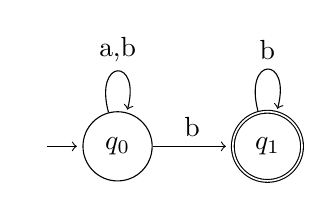
\begin{tikzpicture}[auto, node distance=1cm, shorten >=2pt]
  \node[state,initial,initial text=] (q0) {$q_0$}; 
  \node[state,accepting] (q1) [right=of q0] {$q_1$}; 
  \path[->] 
    (q0) edge [loop above] node {a,b} (q0)
    (q0) edge node {b} (q1)
    (q1) edge [loop above] node {b} (q1);
\end{tikzpicture}

  \end{center}
  And such a language cannot be recognized with a deterministic approach, and this proves that DBA are less expressive than BA.

  \bigskip
  Now, let us show that $L$ \textbf{cannot be recognized by a DBA}.

  Recalling the last proposition, we know that if $L$ is DBA-recognizable it can be expressed as $\overrightarrow{W}$, for some regular set $W$, therefore, we assume that $L = \overrightarrow{W}$ for some regular $W \subseteq A^*$.
  Since $b^\w \in L = \overrightarrow{W}$, it means that we're able to find infinitely many prefixes of $b^\w$ that belong to $W$, in particular there exists a natural number $n_1 \in \w$ \st $b^{n_1} \in W$.
  Since $b^{n_1}ab^\w \in L = \overrightarrow{W}$, it follows that there exists $n_2 \in \w$ \st $b^{n_1}ab^{n_2} \in L$.
  By repeating this step, we can build an \wword of the form $b^{n_1}ab^{n_2}ab^{n_3}a \ldots$ which has infinitely many prefixes in $W$ and thus must belong to $L = \overrightarrow{W}$.
  However, this is a contradiction because such an \wword contains infinitely many occurrences of $a$.
\end{exercise*}

\begin{exercise*}
  Let $A = \set{a,b}$ and let $L = \set{\a \in \Aw: \exists^{\w} n \ \a(n) = a}$.
  Build a BA that recognizes $L$.
  \begin{center}
    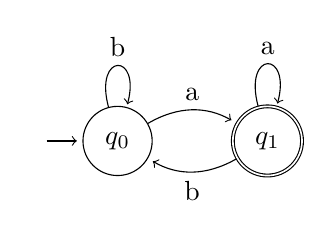
\begin{tikzpicture}[auto, node distance=1cm, shorten >=2pt]
  \node[state,initial,initial text=] (q0) {$q_0$}; 
  \node[state,accepting] (q1) [right=of q0] {$q_1$}; 
  \path[->] 
    (q0) edge [loop above] node {b} (q0)
    (q0) edge [bend left] node {a} (q1)
    (q1) edge [bend left] node {b} (q0)
    (q1) edge [loop above] node {a} (q1);
\end{tikzpicture}

  \end{center}
  The automaton that we build is a particular automaton called \textbf{reset automaton}, where each symbol goes to a single state.
  In this case, reading $b$ we go only in $q_0$, while with $a$ only in $q_1$, no matter the state we're at.

  \textcolor{orange!140}{\rule{\textwidth}{1.5pt}}
  Show that languages recognized by DBA are closed under union.

  \textcolor{orange!140}{\rule{\textwidth}{1.5pt}}

  Show that languages recognized by DBA are closed under intersection.
\end{exercise*}

\begin{proposition*}
  DBA are not closed under complementation, \ie, DBA $\subsetneq$ BA (strictly included).
\end{proposition*}

\section{Muller Automata}

\begin{definition*}[Deterministic Muller Automata (DMA)]
  A DMA is a tuple $\DMA$ where $Q,A,\d,q_0$  are defined as for DBA, while $\F \subseteq 2^Q$, which means that is a subset of the power set of the set of states, \ie, a set of subsets of states.

  \bigskip 
  The computation $\s$ of $\A$ on an \wword $\a$ is successful iff $\infs \in \F$, which means that $\s$ it's successful if the set of all and only the states that occur infinitely many times in the computation belong to $\F$.
  In particular, this means that all the other states must occur finitely many times, leaving us with a very precise characterization of the states.

  \bigskip 
  Definition of acceptance and of $\L(\A)$ are equal to the previous ones.
\end{definition*}

\begin{proposition}[DBA $\subseteq$ DMA]\label{propo:dba_dma}
  Any DBA has an equivalent DMA, \ie, for all DBA there will always exist a DMA that recognize the same language.
\end{proposition}

\begin{proof*}[\nameref{propo:dba_dma}]
    Let $\A = \DBA$ be a DBA.
    The equivalent DMA is $\A' = \DMA$ where $\F = \set{P \in 2^Q: P \cap F \neq \emptyset}$, which means that $\F$ is composed of all and only those subsets of $Q$ that includes at least one final state.

    The computation of the DBA is successful, and this means that the set of states that are encountered infinitely many times is exactly one of the sets in $\F$.
    However, by definition, in $\F$ we have only sets that have a non-empty intersection with $F$, ending with an infinite occurrence of final states.
    This means that to be infinite, there exist at least one final state that occur infinitely many times (otherwise $\F$ would not be infinite, if all occurrences where finite), thus this computation is successful also for the original DBA automaton.
\end{proof*}

NMA can be obtained from DMA by replacing $\d$ with $\D$, and the same construction can be applied to obtain an NMA equivalent to a given BA.

\bigskip
Putting together all that we have seen, we can sum it up with this \emph{temporary} schema:
\begin{equation*}
  \begin{array}{ccc} 
    \text{BA} & \subseteq & \text{NMA} \\
    \rotatebox[origin=c]{90}{$\subsetneq$} & & \rotatebox[origin=c]{90}{$\subseteq$} \\
    \text{DBA} & \subseteq & \text{DMA} 
  \end{array}
\end{equation*}

\begin{proposition}[$\text{BA} \equiv \text{NMA}$]\label{prop:ba_nma}
  BA and NMA are equally expressive.
\end{proposition}

\begin{proof*}[\nameref{prop:ba_nma}]
  On direction have been already proven (BA $\subseteq$ NMA), while the other can be proved by going through S1S, \ie, $\text{NMA} \leadsto \text{S1S} \leadsto \text{BA}$.
\end{proof*}

\begin{lemma}\label{lem:1}
  An \wlan $L \subseteq \Aw$ is recognized by a DMA iff $L$ is a Boolean combination\footnote{Union, Intersection, Complementation} (over the $\Aw$) of languages of the form $\overrightarrow{W}$ where $W$ is a regular language.
\end{lemma}

\begin{note}
  Recall that languages like $\overrightarrow{W}$ can be recognized by deterministic \Buchi automata, but at the same time, DBA are not closed under complementation, thus if we apply complementation we exit from the DBA realm, but we stay in DMA.
\end{note}

The following lemma forces BA to fit into vectorial closure, while by their definition they naturally fit into \wclo:

\begin{lemma}\label{lem:2}
  Every \wlan $L \subseteq \Aw$ which is recognized by an NBA, can be expressed as a finite union of languages of the form $\overrightarrow{U} \cap \overline{\overrightarrow{V}}$, where $U,V \subseteq A^*$ are regular languages.
\end{lemma}
Notice that $\overline{\overrightarrow{V}}$ is the complement of the vectorial closure of $V$.

\begin{question*}[Why proving \autoref{lem:2} isn't easy?]
  Because
  \begin{enumerate}
    \item $U V^\w \neq U \overrightarrow{V}$ in general, even assuming that $V V \subseteq V$.
    \item $U \overrightarrow{V} \neq \overrightarrow{UV}$ in general.
  \end{enumerate}
\end{question*}

\begin{proof*}[1]
  \begin{itemize}
    \item[\color{pink!200}$\Rightarrow$] \ie, we want to prove that $U V^\w \subseteq U \overrightarrow{V}$ with $V V \subseteq V$.

      To prove this, we can simply search for infinite prefixes in $V$ and concatenate them
      \begin{center}
        \begin{tikzpicture}[>=stealth, scale=1.1]

% Axes
\draw[-] (0,0) -- (5.5,0);
\draw[-] (0,-0.1) -- (0,0.1);

\node at (-0.3,0) {$\a$};

% X-axis ticks
\foreach \x in {1,2,3,4,5} {
  \draw (\x,0.1) -- (\x,-0.1);
}

% Ovals from origin to each tick
\foreach \k in {2,3,4} {
  \draw[thick] ({\k/2+1},0) ellipse ({\k/2} and {\k/10+0.5});
}

% labels
\node at (0.5,-0.2) {$\in U$};
\foreach \x in {2,3,4,5} {
  \node at ({\x-0.5},-0.2) {$\in V$};
}
\node at (1.4,0.8) {$\in V$};
\node at (2.4,1.1) {$\in V$};
\node at (3.5,1.1) {$\in V$};

\end{tikzpicture}

      \end{center}
    \item[\color{pink!200}$\Leftarrow$] \ie, we want to prove that $U \overrightarrow{V} \subseteq U V^\w$ with $V V \subseteq V$.

      Let us focus on $V$ and let $V=(ab^*)^*$, then
      \begin{equation*}
        a\underbrace{b \ldots b}_{n_1}a\underbrace{b \ldots b}_{n_2}a\underbrace{b \ldots b}_{n_3}\ldots
      \end{equation*}
      it is immediate to see that $V V \subseteq V$.
      However, if in this language we choose the \wword $ab^\w$, we have that it belongs to $\overrightarrow{V}$ because all its prefixes belong to $V$, but it doesn't belong to $V^\w$ because it doesn't have infinitely-many occurrences of $a$, thus we can conclude that $U \overrightarrow{V} \nsubseteq U V^\w$.
  \end{itemize}
\end{proof*}

\begin{proof*}[2]
  \begin{itemize}
    \item[\color{pink!200}$\Rightarrow$] \ie, we want to prove that $U \overrightarrow{V} \subseteq \overrightarrow{UV}$.

      \begin{center}
        \input{tikz/lemma11_proof_b.tikz}
      \end{center}
      We have that $U$ is always the same and $V$ increases, thus this direction is always true.
  
    \item[\color{pink!200}$\Leftarrow$] \ie, we want to prove that $\overrightarrow{UV} \subseteq U \overrightarrow{V}$.

      The prefix is not fixed and can hypothetically change an infinitely-many times:
      \begin{center}
        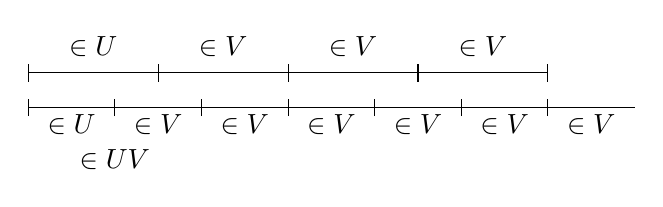
\begin{tikzpicture}[>=stealth, scale=1.1]

\draw[-] (0,0) -- (7,0);
\draw[-] (0,0.4) -- (6,0.4);

% ticks
\draw (0,-0.1) -- (0,0.1);
\foreach \x in {1,2,3,4,5,6} {
  \draw (\x,-0.1) -- (\x,0.1);
  \node at ({\x+0.5},-0.2) {$\in V$};
}
\node at (0.5,-0.2) {$\in U$};

% labels
\foreach \x in {0,1.5,3,4.5,6} {
  \draw (\x,0.3) -- (\x,0.5);
}
\node at (0.75,0.7) {$\in U$};
\node at (2.25,0.7) {$\in V$};
\node at (3.75,0.7) {$\in V$};
\node at (5.25,0.7) {$\in V$};

\node at (1,-0.6) {$\in UV$};

\end{tikzpicture}

      \end{center}
      Following the approach of the picture, we take as a counter case $U = b^*, V = b \andt \a = b^\w$.
      We have that $\overrightarrow{UV} = \{ b^\w \}$, but $U \overrightarrow{V} = \emptyset$ due to having only finite words, so this direction is false and therefore $\overrightarrow{UV} \nsubseteq U \overrightarrow{V}$.
  \end{itemize}
\end{proof*}

\begin{theorem}[McNaughton]\label{thm:mcnaughton}
  An \wlan is \wreg, \ie, recognizable by a NBA, iff it's recognizable by a DMA.
\end{theorem}

\begin{proof*}[\nameref{thm:mcnaughton}]
  \begin{itemize}
    \item[\color{pink!200}$\Rightarrow$] It follows from
      \begin{itemize}
        \item \autoref{lem:2}: characterization of \wreg languages as finite union of expressions of the form $\overrightarrow{U} \cap \overline{\overrightarrow{V}}$;
        \item \autoref{lem:1}: Muller recognizable languages can be expressed as Boolean combinations of vectorial closure of regular sets and vice versa.
      \end{itemize}

    \item[\color{pink!200}$\Leftarrow$] From \autoref{lem:1} (DMA $\implies$ Boolean combinations direction), due to the characterization of the languages recognized by DMA, we can express the language as a Boolean combination of the form $\overrightarrow{V}$, with $V$ regular.
      Then we exploit that any $\overrightarrow{V}$ is recognizable by a DBA and lastly we apply the closure properties of NBA.
  \end{itemize}
\end{proof*}

As a consequence of McNaughton result, the following theorem has been derived:
\begin{theorem}[Expressiveness of WS1S]\label{thm:exp_ws1s}
  An \wlan $L \subseteq \Aw$ is \wreg iff $L$ is definable in WS1S.
\end{theorem}

\begin{proof*}[\nameref{thm:exp_ws1s}]
  \begin{itemize}
    \item[\color{pink!200}$\Rightarrow$] Let $L$ be an \wreg language.
      By McNaughton theorem, $L$ can be expressed as a Boolean combination of languages of the form $\overrightarrow{W}$, with $W$ regular.
      
      $\overrightarrow{W}$ can be captured with an WS1S formula in the following way: using the result on the equivalence of S1S and FSA\footnote{Finite State Automata}, we know that there exists an S1S formula $\p \tuple{\vars{X}{1}{n}}$ that defines $W$.
      It is possible to build a formula $\psi \tuple{\vars{X}{1}{n}, y}$ of WS1S that, when interpreted over \wwords, constrains the prefix of such an \wword up to $y$ to satisfy $\p \tuple{\vars{X}{1}{n}}$.
      To this end, it suffices to relativize second-order quantification to positions less than $y$, like in \autoref{exa:relativization}.
      
      Given the formula of S1S $\p \tuple{\vars{X}{1}{n}}$ that defines $W$, the WS1S formula defining $\overrightarrow{W}$ is
      \begin{equation*}
        \forall x \exists y \Big(x < y \land \psi \tuple{\vars{X}{1}{n}, y} \Big)\ .
      \end{equation*}
  
    \item[\color{pink!200}$\Leftarrow$] Already done. To recall, we can encode any formula of WS1S into S1S by simply constraining the interpretation of quantified second-order variables to be finite.
  \end{itemize}
\end{proof*}

\begin{example}\label{exa:relativization}
  We want to relativize the following formula $\p = \big(\exists X \ (0 \in X)\big)$ to position up to $y$:
  \begin{equation*}
    \exists X \Big(\forall x ( x \in X \to x < y) \land 0 \in X \Big)
  \end{equation*}

  \textcolor{orange!140}{\rule{\textwidth}{1.5pt}}
  We want to relativize the following formula $\p = \big(\forall X \ (0 \in X)\big)$ to position up to $y$:
  \begin{equation*}
    \forall X \Big(\forall x (x \in X \to x < y ) \to 0 \in X \Big)
  \end{equation*}
\end{example}

\section{Rabin Automata}

\begin{definition*}[Rabin Automata (RA)]
  A Rabin Automata is a tuple $\A = \tuple{Q, A, \d/\D, q_0, \O}$ where $\O$ is a set of pairs of subsets of $Q$, \ie, $\set{(L_1, U_1), (L_2, U_2), \ldots, (L_k, U_k)}$ with $L_i, U_i \subseteq Q$ for all $i$.

  \bigskip
  For the acceptance condition of RA, an \wword $\a$ is accepted if a computation $\s$ has
  \begin{gather*}
    \infs \cap L_i = \emptyset \\
    \infs \cap U_i \neq \emptyset
  \end{gather*}
  for some $i$.
  This means that \textit{none} of the states of the first component occurs infinitely-many times (they occur only finitely-many) and \textit{at least one} state in the second component occurs infinitely-many times.
\end{definition*}

From the multiple definitions and theorem we have that $\text{DMA} \equiv \text{DRA}$ and $\text{NBA} \equiv \text{NMA} \equiv \text{NRA}$, plus, for the Safra\footnote{Not explained in the course} theorem, we derive that $\text{NBA} \equiv \text{DRA}$, therefore
\begin{equation*}
  \text{DMA} \equiv \text{DRA} \equiv \text{NBA} \equiv \text{NMA} \equiv \text{NRA}
\end{equation*}
The \textbf{final} schema that collects the expressiveness of the different automata is the following:
\begin{equation*}
  \begin{array}{ccccc} 
    \text{BA} & \equiv & \text{NMA} & \equiv & \text{NRA}\\
    \rotatebox[origin=c]{90}{$\subsetneq$} & \rotatebox[origin=c]{-45}{$\equiv$} & \rotatebox[origin=c]{90}{$\equiv$} & & \rotatebox[origin=c]{90}{$\equiv$} \\
    \text{DBA} & \subsetneq & \text{DMA} & \equiv & \text{DRA}
  \end{array}
\end{equation*}
which essentially means that except DBA, all other classes of automata are equally expressive.

\section{Star-free Languages}

Why single out a class obtained by \emph{removing} an operator? Because star-free languages are precisely the languages definable in \emph{first-order} logic, without second-order quantifiers -- the characterisation made precise by the McNaughton--Papert theorem below, and the linear-time mirror of the first-order fragment of S1S that we meet in the next chapter. Removing the Kleene $^*$ operation, we're losing on the power of second-order variables.

\begin{theorem}[McNaughton and Papert]\label{thm:mcnaughton_papert}
  Let $A$ be a finite alphabet.
  A language $W \subseteq A^*$ is \textbf{star-free} iff it's first-order definable in \SA with the ordering relation $<$.
\end{theorem}

While the successor function $+1$ is definable in terms of $<$, the opposite it's not, \ie, the relation $<$ is only second-order definable in terms of $+1$.
Therefore, \SA with the ordering relation $<$ is strictly more expressive than with the successor function $+1$.

\begin{definition*}[$n$-equivalence]
  The equivalence relation $\eqn$ over $A^*$ is defined for all $u,v \in A^*$, \st

  \bigskip
  \begin{minipage}{0.25\textwidth}
    \hfill
  \end{minipage}
  \begin{minipage}{0.1\textwidth}
    $u \eqn v$
  \end{minipage}
  \begin{minipage}{0.1\textwidth}
    $\iff$
  \end{minipage}
  \begin{minipage}{0.4\textwidth}
    \begin{center}
      $u \andt v$ satisfy the same sentence with quantifier depth $n$
    \end{center}
  \end{minipage}
  \hfill
\end{definition*}

To deal with formulas with free variables, we need to introduce another relation.
The following definition is for 1 free variable:
\begin{definition*}[$(n,1)$-equivalence]
  The equivalence relation $\eqnn$ over $A^* \times \NN$ is defined for all words $u,v \in A^*$ and positions $r,s \in \NN$, \st

  \bigskip
  \begin{minipage}{0.13\textwidth}
    \hfill
  \end{minipage}
  \begin{minipage}{0.25\textwidth}
    $(u,r) \eqnn (v,s)$
  \end{minipage}
  \begin{minipage}{0.1\textwidth}
    $\iff$
  \end{minipage}
  \begin{minipage}{0.45\textwidth}
    \begin{center}
      $(u,r) \andt (v,s)$ satisfy the same formula $\px$ with quantifier depth $n$
    \end{center}
  \end{minipage}
  \hfill

  \bigskip
  where $r,s$ are the positions of the free-variable in $u,v$ respectively, thus $1 \le r \le \abs{u}$ and $1 \le s \le \abs{v}$.
\end{definition*}


These relations, being equivalences, satisfy the reflexive, symmetric and transitive properties.

Moreover, for any $n \ge 1$, both $\eqn \andt \eqnn$ are of finite index, \ie, there exists finitely-many equivalence classes of $\eqn \andt \eqnn$.

Lastly, for any $n \ge 1$, any class $W$ of words $w$ of $\eqn$ can be defined by a sentence $\p_W$ of quantifier depth $n$.
Equally, for $\eqnn$ we will use $\ul{W}$ instead of $W$.

\begin{proposition}\label{prop:1}
  Any formula $\px$ of quantifier depth $n$ is equivalent to a finite disjunction of formulas $\p_{\ul{W}}(x)$, where each formula $\p_{\ul{W}}(x)$ is \st $\ul{W}$ contains some $(u,r)$ that satisfies $\px$.
\end{proposition}

\begin{proposition}\label{prop:2}
  $\eqn \andt \eqnn$ are congruences, \ie:
  \begin{itemize}
    \item if $u \eqn v, u' \eqn v'$, then $uu' \eqn vv'$;
    \item if $u \eqn v, u' \eqn v' \andt a \in A$, then $(uau', \abs{u}+1) \eqnn (vav', \abs{v}+1)$.
  \end{itemize}
\end{proposition}

This second proposition holds also for \textit{non}-finite words.

\begin{proof*}[\nameref{thm:mcnaughton_papert}]
  \begin{itemize}
    \item[\color{pink!200}$\Rightarrow$] This direction it's easier because it exploits the correspondence between the operations $\cup, \bar{\ }, \cdot$ and the quantifiers $\lor, \neg, \exists$.
      For example, given the alphabet $A=\set{a,b,c}$ and an expression
      \begin{equation*}
        A^* \cdot (a \cup c) \cdot (\overline{A^* \cdot b \cdot A^*})
      \end{equation*}
      its star-free version is the following
      \begin{equation*}
        \exists x \Big((x \in Q_a \lor x \in Q_c) \land \neg \exists y (x<y \land y \in Q_b)\Big)
      \end{equation*}
      which is the language of words, with a finite prefix, that after an $a \ort c$ have no occurrences of $b$.

      The proof is done by induction on the structure of star-free expressions.
    \item[\color{pink!200}$\Leftarrow$] This other direction is also done by induction, but on the depth of quantifiers (number of nested quantifiers).
      In particular, we'll focus on the existential, because we can rewrite any universal quantifier in an existential with double negation \big($\forall x\ \px\ \implies\ \neg \exists x\ \neg \px$\big).

      We assume by inductive hypothesis that sentences of depth $n$ can be defined as star-free languages and we consider a formula of the form $\exists x \ \px$ with a depth of $n+1$, 
      This formula can be rewritten as
      \begin{equation*}
        \exists x\ \big(\p_{<x} \land x \in Q_a \land \p_{>x})
      \end{equation*}
      where $\p_{<x}$ refers to positions $< x$, and $\p_{>x}$ the opposite.
      If $\p_{<x}$ and $\p_{>x}$ have quantifier depth $n$, then such a formula describes the language $U \cdot a \cdot V$, where $U \andt V$ are both star-free by inductive hypothesis.

      The hard work consists of rewriting all the formulas into this form, and to do so we will exploit the equivalences just introduced.
      In order to find the star-free counterpart of $\exists x\ \px$, we can restrict our attention to $\exists x\ \p_{\ul{W}} (x)$ instead, because from \autoref{prop:1} it holds that
      \begin{equation*}
        \exists x\ \px \quad \iff \quad \exists x \bigvee_{\ul{W}} \p_{\ul{W}} (x) \quad \iff \quad \bigvee_{\ul{W}} \exists x\ \p_{\ul{W}} (x)
      \end{equation*}
      Now, considering the triple $(U,a,V)$, where $U,V$ are $\eqn$ classes and $a \in A$, if there exist $u_0 \in U, v_0 \in V$ \st $(u_0av_0, \abs{u_0}+1) \in \ul{W}$, then by \autoref{prop:2}, it holds that
      \begin{equation*}
        \forall u \in U, v \in V \qquad (uav, \abs{u}+1) \in \ul{W}
      \end{equation*}
      This means that all words in $U \cdot a \cdot V$ satisfy $\exists x\ \p_{\ul{W}} (x)$, and therefore, $\exists x\ \p_{\ul{W}} (x)$ defines the union of languages $U \cdot a \cdot V$.

      In conclusion, since $U \andt V$ are star-free languages by inductive hypothesis, it follows that $\exists x\ \p_{\ul{W}} (x)$ defines a star-free language.
  \end{itemize}
\end{proof*}

\begin{theorem*}[Ladner]
  Given an alphabet $A$, an \wlan $L \subseteq \Aw$ is first-order definable is \SA iff $L$ is obtained from $\Aw$ by repeated application of Boolean operations and left-side concatenation with star-free languages $W \subseteq A^*$.

  \bigskip
  All the \wlans that satisfy this condition are called \textbf{star-free \wlans}, and are a proper subclass of \wlans, \ie, are strictly less expressive than \wlans.
\end{theorem*}

\section{Fair Transition Systems}

We close the chapter by turning the theory of $\w$-automata onto the systems we actually want to verify. A \textbf{Fair Transition System} models a reactive program, and the reason it belongs \emph{here} is its fairness conditions: \textbf{justice} and \textbf{compassion} both forbid certain behaviors from recurring forever, and ``recurring forever'' is precisely a statement about the set $\inf{\s}$ of states visited infinitely often that we have just studied. The \Buchi automata of this chapter are therefore the natural tool for encoding and checking fairness -- a link we reuse when we model-check these systems later.

\subsection{Definitions}

Fair Transition Systems (FTS) are a way to model reactive programs/systems.

Given a vocabulary $\V$, the \textbf{state of an FTS} is a set of variables in $\V$, which are \textit{typed} (\ie, sorted).
Furthermore, for every variable $u \in \V$ associated to a certain state, there exists another variable $u' \in \V$ which is associated to the next state.

An FTS can be described by means of first-order logic:
\begin{itemize}
  \item \textbf{terms/expressions} are built on variables and constants by applying functions (\eg, successor function);
  \item \textbf{atomic formulas} are either propositional letters or predicates applied to terms;
  \item \textbf{state formulas}, also called assertions, are obtained from atomic ones by applying Boolean connectives and quantifiers.
\end{itemize}
A state is an interpretation of $\V$ that assigns to each variable $u \in \V$ a value $s[u]$, and the set of all the possible states is $\S$, which can be infinite.

\begin{definition*}[Fair Transition System (FTS)]
  A Fair Transition System is a tuple $\tuplev{V, \theta, \T, \J, \C}$ where
  \begin{itemize}
    \item $V$ is the \textbf{set of variables};
    \item $\theta$ is called \textbf{initial condition} is a satisfiable state formula that characterizes the possible initial states, thus a state that satisfies $\theta$ is called \textit{initial state};
    \item $\T$ is a finite \textbf{set of transitions} where each transition $\t \in \T$ is a function that maps each state $s \in \S$ into a set of \tsuc states $\t(s) \subseteq \S$.

      $\t$ is said \textit{enabled} in $s$ if $\t(s) \neq \emptyset$, \ie, $s$ has a \tsuc, otherwise is \textit{disabled};
    \item $\J$ is the set of transitions for which we require \textbf{justice}, or \emph{weak fairness}, which excludes transitions that in some computation may be \textit{constantly enabled} but \textit{never executed}. In other words, if I request something, sooner or later my request must be taken care of;
  \item $\C$ is the set of transitions for which we require \textbf{compassion}, or \emph{strong fairness}, which means that we exclude the existence of computations where these transitions are \textit{enabled infinitely} many times but \textit{executed} only a \textit{finite} number of times.
  \end{itemize}
\end{definition*}

The triple $\tuplev{V, \theta, \T}$ is enough to define a classic transition system, \ie, a graph, while the last two components $\J$ and $\C$ (both $\subseteq \T$) are needed to make the system fair, and thus are called \emph{fairness requirements}.
Moreover, strong fairness implies weak fairness, but not vice versa, and fairness it is not checkable in a ``finite'' way, \ie, by analyzing a finite prefix of a computation.

Each transition $\t \in \T$ can be represented by a formula of FO logic $\rho_\t(V,V')$ called \textbf{transition relation}, which expresses the relationship between a state $s$ and its \tsuc $s'$.
In fact, a state $s'$ is a successor of $s$ via $\t$ if $\rho_\t(V,V')$ evaluates to \true, \ie, $\forall x \in V \; s[x] = \true$.

There exists also a special transition called \textbf{idling transition} and denoted with $\t_I$, which does nothing and doesn't require any fairness condition, and is used to make finite computations infinite, because $\t_I$ is always enabled.
At the same time, to explicitly differentiate transition types, all transitions that are different from $\t_I$ are called \textbf{diligent transitions}.

\begin{definition*}[Computation of an FST]
  An infinite sequence of states $\rho$ is a computation of an FST $P$, or equally is a $P$-computation, if it satisfies the following requirements:
  \begin{itemize}
    \item \textbf{initiality}: $s_0$ is an initial state;
    \item \textbf{consequentiality}: $\forall i \in \NN$, $s_{i+1}$ is a \tsuc of $s_i$ for some $\t$;
    \item \textbf{justice}: $\forall \t \in \J$, it's never the case that, from a position $k$ onwards, $\t$ is constantly enabled but never executed;
    \item \textbf{compassion}:  $\forall \t \in \C$, it's never the case that, from a position $k$ onwards, $\t$ is infinitely enabled but finitely executed.
  \end{itemize}
\end{definition*}

A state is said \textbi{P-accessible} if it occurs in some $P$-computation.
Moreover, each state that is the \tsuc of a $P$-accessible state, is $P$-accessible too.

We call a \textbf{run} of $P$ every infinite sequence $\rho$ that satisfies at least initiality and consequentiality properties.
Every finite prefix of a run is also a prefix of a computation, which means that each state $s$ that occurs in a run is $P$-accessible, and that's because being finite, there will be always a future possibility of making the sequence a computation instead of a run by satisfying the fairness requirements.

\subsection{Simple Programming Language}

The Simple Programming Language (SPL) is a programming language, whose semantic is a FTS.
It's composed of basic instructions, which are:
\begin{itemize}
  \item \texttt{skip}: moves the control after the instruction
  \item \texttt{assignment}
  \item \texttt{await}: waits for the guard to become \true and then it moves the control after the instruction
  \item \texttt{send/receive}: used for synchronous/asynchronous communication
  \item \texttt{request/release}: used for semaphores management over a resource $r$, whose availability must be greater than 0, otherwise no resource is assignable and the request must wait
\end{itemize}

\subsubsection{Schematic instructions}

These type of instructions are sequences of instructions whose termination conditions it's only what matters, and not the details of what they do.
This type is particularly useful for defining:
\begin{itemize}
  \item mutual exclusion: partitions the instructions between critical, that must terminate, and non-critical, where termination isn't required;
  \item producer/consumer paradigm.
\end{itemize}

\subsubsection{Compound/Complex instructions}

Are the following:
\begin{itemize}
  \item conditional: \texttt{if then else};
  \item concatenation: used to execute several instructions in a precise order, one at a time ($s_1;s_2,\ldots$);
  \item selection: unlike concatenation, this instruction selects a subset of enabled instruction to execute (\texttt{when $\ldots$ do});
  \item while: loops an instruction executing until a condition is satisfied (\texttt{while $\ldots$ do});
  \item cooperation: parallel execution of a set of instructions;
  \item block: allows local declaration of variables used by the block instructions.
\end{itemize}

\subsubsection{Group composite instructions}

These instructions are used to make some compound instructions atomic, \ie, executable as if it was a single instruction, in a single step. This is achieved by the adoption of the so-called composite instructions.

\subsubsection{Program}

The syntax of a program is the following
\begin{equation*}
  P :: [ \text{declaration}; [P_1 :: [I_1 : S_1; \widehat{I}_1 : ] \Vert \ldots \Vert P_k :: [I_k : S_k : \hat{I_k} ]]]
\end{equation*}
where the names of the program and of the processes, respectively $P$ and $P_i$ are optional.
The declaration is a list of instructions of the form
\begin{equation*}
  \texttt{mode } \text{var}_1, \ldots, \text{var}_n : \texttt{type } \text{where } \p
\end{equation*}

\begin{note}
  This part isn't complete; go check the slides on SPL.
\end{note}

\bigskip
We now have two complementary, \emph{operational} views of infinite behavior: $\w$-automata, which \emph{recognise} $\w$-languages, and fair transition systems, which \emph{generate} them. What is still missing is a \emph{declarative} language in which to \emph{state} the properties we want such behaviors to have. The next chapter supplies one and -- remarkably -- shows it has \emph{exactly} the expressive power of the automata we have just built.

\chapter{Monadic Second-Order Logic}

\Buchi automata give an \emph{operational} description of an $\w$-language -- a recipe for recognising it. The monadic second-order theory of one successor (S1S) gives a \emph{declarative} one -- a property that characterises it. Why connect the two? Because logic is how we will naturally \emph{write specifications}, while automata are how we will \emph{decide} them; the bridge between writing and deciding is the central result of this chapter, \Buchi's theorem: \textbf{an $\w$-language is \wreg if and only if it is definable in S1S}. This is the $\w$-word analogue of Kleene's theorem, and it is what makes logical specification \emph{decidable}.

\section{\SA and S1S}

In this section are explained the relationship between \Buchi automata and \textbf{Second-order monadic theory of One Successor} (S1S).
The most important result is the equivalence between $\w$-regularity and definability in S1S.
We're going to show how these formalisms, in particular the S1S formulas, can be used as a tool to define languages, and how the power of decidability of these is the same of \Buchi automata.

Let $A$ be an alphabet (finite set).
We denote with \SA the application of the S1S formalism to a specific alphabet $A$.

\begin{definition*}[\SA]
  \SA is defined as follows:
  \begin{itemize}
    \item terms are obtained from the constant 0 and first-order variables ($x,y,z \ldots$) by possibly applying the successor function ($+1$);
    \item atomic formulas have one of the following forms:
      \begin{itemize}
        \item $t_1 = t_2$, \ie, terms equality
        \item $t_1 < t_2$, \ie, natural ordering of terms
        \item $t_1 \in X$, where $X$ is a second-order\footnote{Not a single element of a domain, but a set of elements of a domain} variable,\ie, is a set of variables (natural numbers)
        \item $t_1 \in Q_a$, where $Q_a$ is the set of all the positions where the $a$ occurs in an infinite word, and $t_1$ is associated to one of these positions. For all $a \in A$, $Q_a$ is a symbol for a unary predicate.
      \end{itemize}
      Note that the interpretation of the first two formula's forms is fixed, while for the last two it changes depending on the choice of \wword.
    \item formulas of \SA are obtained from atomic formula by possibly applying Boolean formulas connectives $(\land, \lor, \neg)$ and quantifiers $(\forall, \exists)$ over first-order and second-order variables (\eg, $\forall x, \exists y, \forall Y$).
  \end{itemize}
\end{definition*}

An \emph{open} formula is when we have at least one free variable, which is a variable not linked to a quantifier, thus the interpretation of the formula depends on the free variables.
On the other hand, a \emph{closed} formula is a formula with no free variables, therefore the interpretation is fixed, doesn't change.

Some elements of \SA are redundant:
\begin{itemize}
  \item the constant 0, because we can redefine the 0 as a variable $x$ with the formulas
  \begin{equation*}
    \forall y \quad x=y \lor x < y
  \end{equation*}
  or
  \begin{equation*}
    \neg\exists y \quad y+1 = x
  \end{equation*}
  and that's because these formulas are satisfied only if $x=0$;
  \item $+1$ and $<$ are interdefinable because we can write $x=y+1$ as
  \begin{equation*}
    y<x\ \land\ \neg \exists z \left( y<z \land z<x \right)
  \end{equation*}
  \item the ordering operator $<$, because $x<y$ can be redefined as
    \begin{equation*}
      \forall X \left[ x+1 \in X \land \forall z \left( z \in X \to z+1 \in X \right) \to y \in X \right]
    \end{equation*}
    which means that if we have an $x \in X$, then we have successor $x+1 \in X$, therefore this successor will have its own successor which will also be in $X$, and thus somewhere will have a successor equal to $y$, which means that $y \in X$.
    Alternatively
    \begin{equation*}
      \exists X \left[ x \notin X \land (x+1) \in X \land \forall z \left( z \in X \to z+1 \in X \right) \land y \in X \right]
    \end{equation*}
\end{itemize}

\begin{definition*}[Model theoretic interpretation of $\w$-words]
  Let $\a \in \Aw$, its model-theoretic interpretation is
  \begin{equation*}
    \underline{\a} = \left( \w, 0, +1, <, \left\{ Q_a \right\}_{a \in A} \right)
  \end{equation*}
  where $\w$ is the set of natural numbers and $Q_a = \left\{ i \in \w: \a(i) = a \right\}$.
  
  Given a sentence\footnote{A sentence is a closed formula} $\p$ of \SA, the language defined by $\p$ is $L\left( \p \right) = \left\{ \a\in \Aw: \underline{\a} \models \p \right\}$.
\end{definition*}

\begin{note}
  Even though it's specified sentence, it is a sentence for the S1S formalism, but has some degree of freedom because the interpretation of $Q_a,Q_b,Q_c,\ldots$ depends on the choice of \wword.
\end{note}

\begin{example*}
  Given $A = \set{a,b,c}$, the language $L$ that includes all and only those \wwords \st every occurrence of an $a$ is sooner or later followed by an occurrence of a $b$ is
  \begin{equation*}
    \forall x\ [\, x \in Q_a \to \exists y ( y \in Q_b \land x<y ) \,]
  \end{equation*}
\end{example*}

\begin{example*}
  Given $A = \set{a,b,c}$, the language that includes only those \wwords where the number of $b$ and $c$ in between $a$ is even, is
  \begin{align*}
    \forall x,y\ [&x \in Q_a \land y \in Q_a \land x<y \land \\
                  &\neg\exists z \left( x<z \land z<y \land z \in Q_a \right) \to \exists X \left( x \in X \land \forall z \left( z \in X \leftrightarrow z+1 \notin X \right) \land y \notin X \right) ]
  \end{align*}
\end{example*}

It's possible to generalize the \SA definition, removing the dependency between each $Q_{\_}$ to a specific symbol of the alphabet $A$ (\eg, $a,b,c,\ldots$).
To do so, we just need to change the representation of the symbols of our alphabet $A$ to $\set{0,1}^n$, where $n = \lceil \log_2 \abs{A} \rceil$.
With this notation we can encode each symbol of $A$ to a string of $0$s and $1$s (binary value), and therefore represent each symbol concurrently.
In this way, we don't need to specify the formalism for each alphabet $A$, but we have now a general representation that is sufficient to express every possible alphabet.
The generalized version of \SA is simply denoted with S1S.
The model-theoretic interpretation now becomes
\begin{equation*}
  \underline{\a} = \left( \w, 0, +1, <, \left\{ P_i \right\}_{i = 1,\ldots,n}  \right)
\end{equation*}
where $\left\{ P_i \right\}$ is the interpretation of $X_i$, and $P_k = \set{i \in \w : (\a(i))_k = 1}$ for all $k = 1,\ldots,n$.
It's immediate to see that sentences of \SA can be replaced by an equivalent formula $\psi(X_1, \ldots,\allowbreak X_n)$.

\begin{theorem}[Closure under projection]\label{thm:proj_closure}
  Let $\psi(\vars{X}{1}{i-1},\vars{X}{i+1}{n})$ be an S1S formula of the form:
  \begin{equation*}
    \exists X_i \quad \p(\vars{X}{1}{n})
  \end{equation*}
  This means that $\psi$ is obtained from $\p$ by existentially closing one of its second-order variables.

  \bigskip
  If $\L(\p)$ is \wreg, then $\L(\psi)$ is \wreg as well.
\end{theorem}

\pagebreak

\begin{proof}[\nameref{thm:proj_closure}]\label{prf:proj_closure}
  Let $\A$ be a BA for $\p$, that is $\L(\A) = \L(\p)$.
  We show how to obtain a \Buchi automaton $\A'$ for $\psi$.

  \begin{center}
    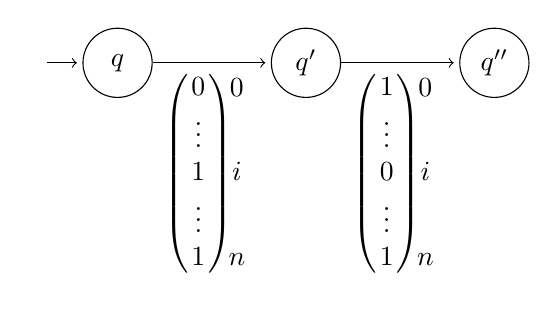
\begin{tikzpicture}[auto, node distance=1.5cm, shorten >=2pt]
  \node[state,initial,initial text=] (q0) {$q$}; 
  \node[state] (q1) [right=of q0] {$q^\prime$}; 
  \node[state] (q2) [right=of q1] {$q^{\prime\prime}$}; 
  \path[->] 
    (q0) edge node [swap] {$\left( \hspace{-4pt}\begin{array}{c} 0 \\ \vdots \\ 1 \\ \vdots \\ 1 \end{array} \hspace{-4pt}\right) \hspace{-8pt}\begin{array}{c} 0 \\[0.65cm] i \\[0.65cm] n \end{array}$} (q1)
    (q1) edge node [swap] {$\left( \hspace{-4pt}\begin{array}{c} 1 \\ \vdots \\ 0 \\ \vdots \\ 1 \end{array} \hspace{-4pt}\right) \hspace{-8pt}\begin{array}{c} 0 \\[0.65cm] i \\[0.65cm] n \end{array}$} (q2);
\end{tikzpicture}

  \end{center}

  The BA $\A'$ can be obtained from $\A$ by simply removing the $i$-th component from each label of edges\footnote{This is not a problem thanks to non-determinism of BA}.
\end{proof}

In \autoref{prf:proj_closure} non-determinism of BA is essential.
It's also very important to notice that only one second-order variable is existentially closed.
In fact, if all second-order variables had been existentially closed ($\vars{\exists X}{1}{n} \allowbreak \p(\vars{X}{1}{n})$), this would have led to transitions without labels associated, and this is a special type of automaton called \textbf{input-free automaton}.

\section{\Buchi theorem and $\text{S1S}_0$}

\begin{theorem}[\Buchi]\label{thm:buchi}
  An \wlan $L \subseteq \Aw$ is \wreg iff it's definable in S1S.
\end{theorem}

\begin{proof*}[\nameref{thm:buchi}]
  \begin{itemize}
    \item[\color{pink!200}$\Rightarrow$] Let $\A = \tuple{Q,A,\D,q_0,F}$ be a BA that recognizes an \wlan L over A.
      Let us assume that $Q = \set{0,\ldots,m}$ and $q_0 = 0$.

      We write a sentence of \SA of the form
      \begin{equation*}
        \vars{\exists Y}{0}{m} \quad \p(\vars{Y}{0}{m})
      \end{equation*}
      where each $Y_i$ is used to identify the position of the $i$-th step.
      For all $\a \in \Aw$, $\underline{\a}$ is a model for the above formula iff $\a$ is accepted by $\A$.

      $\p$ consists of three conjuncts:
      \begin{enumerate}
        \item The initial state starts from $q_0$ and at each position of the computation there is at most one state (uniqueness of states):
          \begin{equation*}
            \p_1(\vars{Y}{0}{m}) = \quad 0 \in Y_0 \quad \land \quad \bigwedge_{i \neq j} \neg\exists y \left( y \in Y_i \land y \in Y_j \right)
          \end{equation*}
        \item the second conjunct states consequentiality, \ie, we can go from one state to another only if there is a transition in the $\D$ that justifies this transition:
          \begin{equation*}
            \p_2(\vars{Y}{0}{m}) = \quad \forall x \bigvee_{\tuple{i,a,j} \in \D} \left( x \in Y_i \land x \in Q_a \land x+1 \in Y_j \right)
          \end{equation*}
        \item the last ensures that we're able to encode the \textbf{acceptance condition} of \Buchi automata by means of an S1S formula.
          To specify the acceptance condition we can say that there exists at least one final state and that we can encounter it, during the computation, infinitely many times.
          \begin{equation*}
            \p_3(\vars{Y}{0}{m}) = \quad \bigvee_{i \in F} \forall x \exists y \left( x<y \land y \in Y_i \right)
          \end{equation*}
      \end{enumerate}

      Supposing that we have already proved also the other direction of the proof ($\Leftarrow$), we would be able to do
      \begin{equation*}
        \p \in \text{S1S} \leadsto\footnote{Direction $\Leftarrow$} \quad \text{BA } \A \leadsto\footnote{Direction $\Rightarrow$} \quad \overline{\p} \in \text{S1S}
      \end{equation*}
      ending with a normal form for S1S formulas.
  \end{itemize}
\end{proof*}

Before starting with the other side of the proof, we want to simplify the form of S1S to make the proof easier, by introducing an equally expressive type $\text{S1S}_0$, and replace S1S with it.

\begin{definition*}[$\text{S1S}_0$]
  $\text{S1S}_0$ has only second-order quantification and variables, plus atomic formulas are restricted to the forms:
  \begin{itemize}
    \item $X \subseteq Y$, which means inclusion of second-order variables, \ie, the set of natural numbers associated with $X$ must be a subset of the set of natural numbers associated with $Y$
    \item $\succxy$, which stands for successor and it means $X=\set{x}, Y=\set{y} \andt x+1 = y$
  \end{itemize}
\end{definition*}

\begin{theorem*}
  S1S and $\text{S1S}_0$ are equally expressive.
\end{theorem*}

\begin{proof*}
  \begin{itemize}
    \item[\color{pink!200}$\Leftarrow$] ($\text{S1S}_0 \to \text{S1S}$)
      \begin{itemize}
        \item $X \subseteq Y$ can be rewritten in S1S form as $\forall x \left( x \in X \to x \in Y \right)$
        \item the successor function $\succxy$ can be rewritten in S1S form as 
          \begin{align*}
            \exists x \exists y \Big( &x \in X \land y \in Y \\
              &\land \neg\exists x' (x' \neq x \land x' \in X) \\
              &\land \neg\exists y' (y' \neq y \land y' \in Y) \\
              &\land x+1 = y \Big)
          \end{align*}
      \end{itemize}
    \pagebreak
    \item[\color{pink!200}$\Rightarrow$] ($\text{S1S} \to \text{S1S}_0$)
      To show this, it's useful to introduce some notation:
      \begin{itemize}
        \item $X = Y$ means that $X \subseteq Y \land Y \subseteq X$
        \item $\sing{x}$ represents the singleton set and it means that
          \begin{equation*}
            \exists Y \Big( Y \subseteq X \land Y \neq X \land \neg\exists Z (Z \subseteq X \land Z \neq X \land Z \neq Y) \Big)
          \end{equation*}
      \end{itemize}
      \vspace{-5pt}
      Furthermore, to go from \text{S1S} to $\text{S1S}_0$, we have to:
      \begin{itemize}
        \item eliminate 0 and ordinary relation < ;
        \item +1 occurs only in formulas of the form $x+1 = y$;
      \end{itemize}
      and this means that in this setting, atomic formulas can have only the following forms:
      \begin{itemize}
        \item $x = y$, which can be rewritten in $\text{S1S}_0$ form as $X = Y \land \sing{X} \land \sing{Y}$
        \item $x+1 = y$, which can be rewritten in $\text{S1S}_0$ form as $\succxy$\footnote{There is no need to specify that $X$ and $Y$ are singletons, because this is already included in the definition of successor}
        \item $x \in X$, which can be rewritten in $\text{S1S}_0$ form as $Y \subseteq X \land \sing{Y}$
      \end{itemize}
      Lastly, we also need to remove universal/existential quantifiers of first-order variables ($\forall x, \exists x$), but that's an easy process because we just need to replace the first-order variables with second-order ones, and then require them to be interpreted as singletons:
      \vspace{-10pt}
      \begin{align*}
        & \exists x \left( \ldots \right) \quad \leadsto \quad \exists X \Big( \sing{X} \land \ldots \Big) \\
        & \forall x \left( \ldots \right) \quad \leadsto \quad \forall X \Big( \sing{X} \to \ldots \Big)
      \end{align*}
  \end{itemize}
\end{proof*}

An example of transformation is:
\begin{equation*}
  \forall x \exists y (x+1=y\;\land\; y \in Z) \qquad \leadsto \qquad \forall X \Big( \sing{X} \to \exists Y (\sing{Y} \land \succxy \land Y \subseteq Z) \Big)
\end{equation*}

The mapping of S1S formula into BA is defined inductively on the structure of the formula (the two above).
The base cases are inclusion and successor, and that's why we introduced $\text{S1S}_0$.

\begin{proof*}[\nameref{thm:buchi}]
  \begin{itemize}
    \item[\color{pink!200}$\Leftarrow$] 
      \textit{Base cases}:
      \vspace{-10pt}
      \begin{itemize}
        \item $X \subseteq Y$ \qquad \qquad \eg,
          \begin{tabular}{c|c|c|c|c|c} 
            $X$ & 0 & 0 & 1 & 1 & 1\\
            \hline
            $Y$ & 1 & 0 & 1 & 0 & 0
          \end{tabular}

          And the automata that recognizes $X \subseteq Y$ it's trivial, because we just have to check that any index in $X$ is also an index in $Y$.
          \begin{center}
            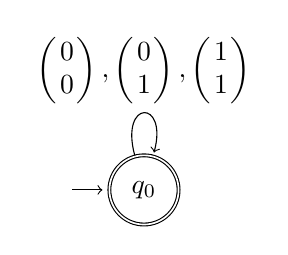
\begin{tikzpicture}[auto, node distance=1.5cm, shorten >=2pt]
  \node[state,initial,initial text=,accepting] (q0) {$q_0$}; 
  \path[->] 
    (q0) edge [loop above] node {$\left(\hspace{-4pt}\begin{array}{c} 0 \\ 0 \end{array}\hspace{-4pt}\right),\left(\hspace{-4pt}\begin{array}{c} 0 \\ 1 \end{array}\hspace{-4pt}\right),\left(\hspace{-4pt}\begin{array}{c} 1 \\ 1 \end{array}\hspace{-4pt}\right)$} (q0);
\end{tikzpicture}

          \end{center}
        \item $\succxy$

          And the automata that recognizes it is:
          \begin{center}
            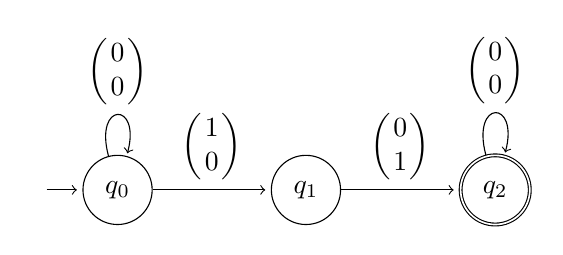
\begin{tikzpicture}[auto, node distance=1.5cm, shorten >=2pt]
  \node[state,initial,initial text=] (q0) {$q_0$}; 
  \node[state] (q1) [right=of q0] {$q_1$}; 
  \node[state,accepting] (q2) [right=of q1] {$q_2$}; 
  \path[->] 
    (q0) edge [loop above] node {$\left(\hspace{-4pt}\begin{array}{c} 0 \\ 0 \end{array}\hspace{-4pt}\right)$} (q0)
    (q0) edge node {$\left(\hspace{-4pt}\begin{array}{c} 1 \\ 0 \end{array}\hspace{-4pt}\right)$} (q1)
    (q1) edge  node {$\left(\hspace{-4pt}\begin{array}{c} 0 \\ 1 \end{array}\hspace{-4pt}\right)$} (q2)
    (q2) edge [loop above] node {$\left(\hspace{-4pt}\begin{array}{c} 0 \\ 0 \end{array}\hspace{-4pt}\right)$} (q2);
\end{tikzpicture}


          \end{center}
      \end{itemize}
      
      \textcolor{pink!160}{\rule{\textwidth-30pt}{1pt}}

      \textit{Inductive step}:
      In conclusion of this proof, it suffices to recall that BA are closed under intersection ($\p_1 \land \p_2$), union ($\p_1 \lor \p_2$), complementation ($\neg \p_1$) and projection ($\exists X \p_1$).
  \end{itemize}
\end{proof*}

Having proved this, now we know that from now on, everything that BA captures, it can be recognized as well by S1S, and vice versa.

\begin{theorem*}[\Buchi theorem finite]
  \Buchi theorem can be proved also in the finite case, with small changes.
  Given $\a \in A^*$ of the length $k+1$, we have
  \begin{equation*}
    \underline{\a} = \big(\set{0,\ldots,k}, \emptyset, +1, <, \set{P_i}_{i=1,\ldots,n} \big)
  \end{equation*}
  where $P_l = \set{ i \in \set{0,1,\ldots,k}: \left( \a(i) \right)_l = 1 }$, \ie, we collect in $P_l$ all those positions between 0 and $k$, \st the $l$ component of the tuple at position $i$ is equal to 1.
  
  The problems with this are
  \begin{itemize}
    \item when it's applied the successor function to the maximum element. To solve it, we have to redefine the successor $+1$ at position $k$, and we do it by defining $k+1$ as $k$ to remain in $k$;
    \item we have to take into account the empty word $\e$.
      To do so, we assume that $\e$ cannot be used to satisfy any existential statement, while with universal quantificators, the argument is true for the empty word $\e$.
      In this way it cannot satisfy any existential quantification and falsify any universal quantification.
  \end{itemize}
  We also restrict second-order quantification over finite sets.
\end{theorem*}

\begin{corollary*}
  A language $L \subseteq A^*$ is regular iff is definable in S1S in the finite setting.
\end{corollary*}

The theory S1S is the set of sentences which are satisfied in the structure $\tuple{\w, \emptyset, +1, <}$.
For example:
\begin{align*}
  & \forall X \exists Y \forall x \left( x \in X \to x \in Y \right) \qquad \true \\
  & \forall X \exists y \forall x \left( x \in X \to x < y \right) \qquad \false
\end{align*}

\begin{corollary*}
  The theory S1S is decidable.
\end{corollary*}

\section{WS1S}

Membership in the theory S1S is non-elementary.
For example:
\begin{align*}
  & \exp_0(n) = n \\
  & \exp_1(n) = 2^n \\
  & \exp_2(n) = 2^{2^n} \\
  & \exp_{h+1}(n) = 2^{\exp_h(n)}
\end{align*}
so essentially we have that $\exp_h(n) = 2^{2^{\dots^{2^n}}}$, where the number (the height) of exponentiations is $h$.
A problem is \textbf{non-elementary} when it's not possible to find a bound to the number of exponentiations.

The membership problem of $\p$ in S1S is non-elementary, but at the same time non-emptiness for $\A$ in BA is trivial because it's solvable in polynomial time.
Still, the two problems are linked together, and the cause behind such difference in the complexity stands in the translation of $\p$ into $\A$, which may involve a non-elementary blow up in the size of the automaton.

In terms of S1S formulas, we can think of $n$ as the size of the formula and $h$ as the number of alternations of existential/universal blocks, having the following form
\begin{equation*}
  \exists \exists \ldots \exists \forall \ldots \forall \exists \ldots \exists
\end{equation*}
which can be rewritten to use only existential quantifiers by replacing $\forall$ blocks with $\neg\exists$, like this
\begin{equation*}
  \exists \exists \ldots \exists \neg \exists \ldots \exists \neg \exists \ldots \exists
\end{equation*}
The ``height'' of the exponentiation tower will be equal to the number of alternations between existential/universal quantifiers, or in the rewritten formula, to the number of negations.

As a matter of fact, \Buchi considered a weaker variant of S1S called \textbf{Weak S1S} (WS1S).

\begin{theorem*}
  The theory S1S and WS1S are equivalent.
\end{theorem*}

\begin{proof*}
  \begin{itemize}
    \item[\color{pink!200}$\Leftarrow$] WS1S can be defined as S1S by constraining second-order quantified variables to be interpreted as finite sets
      \begin{equation*}
        X \qquad \to \qquad X = \emptyset \lor \exists x \big(x \in X \land \forall y (x<y \to y \notin X)\big)
      \end{equation*}
      From this, decidability of WS1S immediately follows, because we can take any formula of WS1S, rewrite it as a formula of S1S as described and then use \Buchi automata to decide it.
    \item[\color{pink!200}$\Rightarrow$] It's more difficult, therefore we're not showing the entire proof, but just a sketch.
      In S1S we work over sets of the form $W^\w$, because the way we build \wwords is by applying the \wclo (concatenation of an infinite number of finite words).
      The counterpart for WS1S for generating \wwords is the vectorial closure $\overrightarrow{W}$, \ie, \wwords which consists of infinitely many finite prefixes belonging to $W$.
  \end{itemize}
  In short, the direction WS1S~$\to$~S1S is purely syntactic (WS1S is a fragment of S1S), whereas the converse -- that every S1S formula can already be written weakly -- is \emph{not} elementary: it rests on the automata-theoretic equivalence $\text{NBA} \equiv \text{DMA}$ (\autoref{thm:mcnaughton}), which is what lets a vectorial closure $\overrightarrow{W}$ stand in for an $\w$-closure $W^\w$.
\end{proof*}

\section{Extensions of S1S}

S1S can be extended with a suitable unary predicate preserving decidability.

\begin{example*}
  Examples of possible extension predicate are:
  \begin{itemize}
    \item the predicate is a power of $k$, in particular, a power of 2
    \item the predicate is a factorial
  \end{itemize}
\end{example*}

Decidability is \textbf{lost} if you add the function $f(x) = 2x$ because, in order to represent this function, you must use a binary relation between $x$ and $f(x)$.
Instead, an extension that \textbf{preserves} decidability it's the one proposed by Rabin, which replaces the successor function +1 with two successors $+_0 1$ and $+_1 1$, and it's called infinite binary tree theory S2S.

\begin{center}
  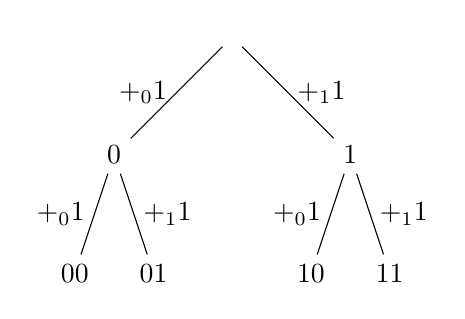
\begin{tikzpicture}[
  level 1/.style={sibling distance=3cm},
  level 2/.style={sibling distance=1cm}]
  \node (Root) {$\e$}
      child {
          node {0}
          child { node {00} edge from parent node[left] {$+_0 1$} }
          child { node {01} edge from parent node[right] {$+_1 1$} }
          edge from parent node[left] {$+_0 1$}
      }
      child {
          node {1}
          child { node {10} edge from parent node[left] {$+_0 1$} }
          child { node {11} edge from parent node[right] {$+_1 1$} }
          edge from parent node[right] {$+_1 1$}
      };
\end{tikzpicture}

\end{center}

\section{S2S and Tree Automata}

In this setting, we'll work with infinite binary trees to represent infinite words, where each node represents a possible symbol choice.
An example of a tree is over $A=\set{0,1}$ is
\begin{center}
  \begin{tikzpicture}
  [level 1/.style={sibling distance=3cm},
  level 2/.style={sibling distance=1cm}]
  \node at (0,0) {$\e$}
      child {
          node {0}
          child {
            node {00}
            child { node {000} }
            child { node {001} }
          }
          child { node {01} }
      }
      child {
          node {1}
          child { node {10} }
          child { node {11} }
      };
  \node at (1,-4) {$\dots$};
\end{tikzpicture}

\end{center}
and, in this case, the \wwords in it are defined as $t: \text{dom}(t) \to A^*$, where dom(\_) is the function that represents the tree.

There is no difference in expressiveness between a binary tree and a $k$-ary tree, \ie, a tree where each node has at most $k$ children, thus the number branches is not fixed, because we can encode any $k$-ary tree into a binary one.

\bigskip
S2S is obtained from S1S by:
\begin{itemize}
  \item replacing 0 with $\e$;
  \item replacing $+1$ with $\succ_0 \andt \succ_1$, which are respectively the left and right children;
  \item modifying the ordering relation $<$ to be a partial relation called \textbf{prefix relation}. It's not total because we can only compare two words based on the same prefix, \ie, the same path, but we can't compare words on different paths (\eg, $001 < 00101$ while $0100\ ?\ 101$). However, a trick to make it total is to use the lexicographical order.
\end{itemize}

Here are implemented some examples of functions:
\begin{itemize}
  \item $\text{chain}(X)\!: \forall x, y \in X \quad x<y \lor y<x \lor x=y$, \ie, a set of nodes that are prefix ordered, \eg, $\set{0, 00, 001, 00100, 0010001}$;

  \item $\text{path}(X)\!: \text{chain}(X) \land\, \nexists Y\, \big(X \subseteq Y \land X \neq Y \land\, \text{chain}(Y)\big)$, \ie, a particular chain, called \emph{maximal chain}, that have no missing nodes in the middle, \eg, $\{0, 00, 001, 0010, 00100, 0010$-\\$00, 0010001\}$;

  \item The lexicographical order can be implemented as $x \preceq y: x \leq y \lor \exists z\, ( z0 \leq x \land z1 \leq y )$, where $\le$ is an extension of the prefix relation which means ordering or equal, and $z0,z1$ are respectively the left and right children ($z$ concatenated $0/1$). An example of application of the lexicographical ordering relation is $011 \preceq 10$.
\end{itemize}

We want to define automata over trees, in particular NBA and NRA.

\begin{definition*}[NBA over trees]
  A NBA that works over trees is a tuple $\A = \NBA$ where $\D \subseteq Q \times A \times Q \times Q$, \ie, the combination of current state, current symbol and state for left and right children.
  
  \bigskip
  We denote with $T^w_A$ the set of all infinite binary trees over alphabet $A$.

  A run $r$ of $\A$ on a tree $t \in T^w_A$ is a map $r: \set{0,1}^* \to Q$, \st
  \begin{itemize}
    \item initiality: $q_0 = r(\e)$;
    \item consequentiality: $\big( r(w), t(w), r(w0), r(w1)\big) \in \D$.
  \end{itemize}
  The run is successful if for all paths $\pi$ it holds that $\inf{\pi} \cap F \neq \emptyset$.
\end{definition*}

\begin{definition*}[NRA over trees]
  A NRA that works over trees is a tuple $\A = \NRA$ where $\O = \{\,(L_1,U_1), \ldots,\allowbreak (L_n,U_n)\,\}$.
  
  \bigskip
  The run $r$ is successful if for all paths $\pi$ there exists a pair $(L_j,U_j)$ \st $\inf{\pi} \cap L_j = \emptyset \andt \inf{\pi} \cap U_j \neq \emptyset$, \ie, the state in the first component must occur finitely many times, while the state in the second must occur infinitely many times.
\end{definition*}

\begin{theorem}[NBA $\mapsto$ NRA]\label{thm:nba_nra}
  Any NBA can be converted into an NRA, but not vice versa.
\end{theorem}

\begin{proof*}[\nameref{thm:nba_nra}]
  Given a NBA $\A = \NBA$, it's possible to obtain an equal NRA $\A' = (\,Q, A, \D,\allowbreak q_0, \O\,)$ by making $\O$ equal to $\set{(\emptyset, F)}$.
\end{proof*}

\begin{exercise}\label{ex:tree_t0}
  Given an alphabet $A = \set{a,b}$ and a language of trees $T_0 = \set{t \in \Twa \mid \text{some path} \allowbreak \text{through $t$ carries infinitely many $a$}}$.
  Starting equally from $a$ or $b$, we have to chose which side to take (left or right), but we don't know if the correct path is on the left subtree or right, therefore to stay general, we split the tree in two and in the first we mark the left subtree as final, while on the second the let the right subtree to be the final one.
  \begin{center}
    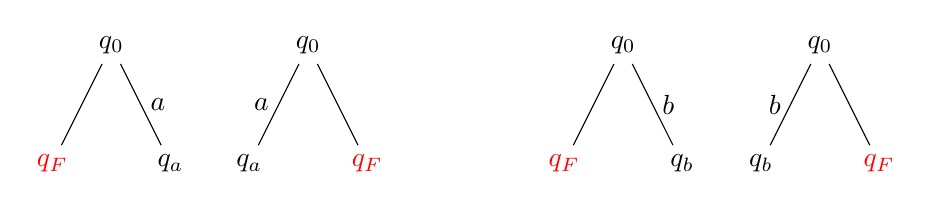
\begin{tikzpicture}
  \node at (-4.5,0) {$q_0$}
    child{
      node {\color{red}$q_F$}
    }
    child{
      node {$q_a$}
      edge from parent node[right] {$a$}
    };

  \node at (-2,0) {$q_0$}
    child{
      node {$q_a$}
      edge from parent node[left] {$a$}
    }
    child{
      node {\color{red}$q_F$}
    };

  \node at (2,0) {$q_0$}
    child{
      node {\color{red}$q_F$}
    }
    child{
      node {$q_b$}
      edge from parent node[right] {$b$}
    };

  \node at (4.5,0) {$q_0$}
    child{
      node {$q_b$}
      edge from parent node[left] {$b$}
    }
    child{
      node {\color{red}$q_F$}
    };
\end{tikzpicture}

  \end{center}
  When we go into a final subtree, marked with $q_F$, we're not interested in what symbol we read, while, on the other branch, we specify with $q_a \ort q_b$ respectively if we read $a \ort b$.
  We can proceed with this approach and always expand only in one direction:
  \begin{center}
    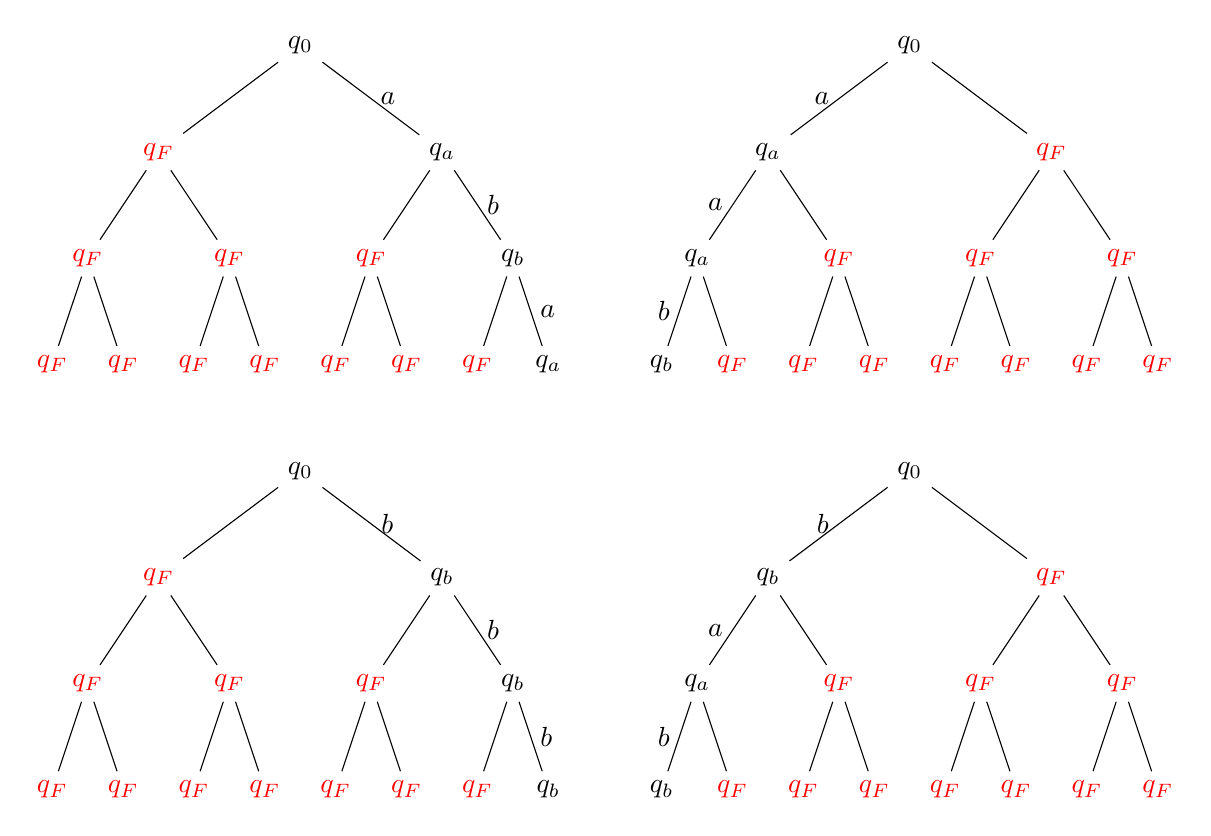
\begin{tikzpicture}
[
  scale=0.9,
  level 1/.style={sibling distance=4cm},
  level 2/.style={sibling distance=2cm},
  level 3/.style={sibling distance=1cm}
]
  \node at (-4.3,3) {$q_0$}
    child{
      node {\color{red}$q_F$}
      child{
        node {\color{red}$q_F$}
        child { node {\color{red}$q_F$}}
        child { node {\color{red}$q_F$}}
      }
      child{
        node {\color{red}$q_F$}
        child { node {\color{red}$q_F$}}
        child { node {\color{red}$q_F$}}
      }
    }
    child{
      node {$q_a$}
      child{
        node {\color{red}$q_F$}
        child { node {\color{red}$q_F$}}
        child { node {\color{red}$q_F$}}
      }
      child{
        node {$q_b$}
        child { node {\color{red}$q_F$}}
        child { node {$q_a$} edge from parent node[right] {$a$}}
        edge from parent node[right] {$b$}
      }
      edge from parent node[right] {$a$}
    };

  \node at (4.3,3) {$q_0$}
    child{
      node {$q_a$}
      child{
        node {$q_a$}
        child { node {$q_b$} edge from parent node[left] {$b$}}
        child { node {\color{red}$q_F$}}
        edge from parent node[left] {$a$}
      }
      child{
        node {\color{red}$q_F$}
        child { node {\color{red}$q_F$}}
        child { node {\color{red}$q_F$}}
      }
      edge from parent node[left] {$a$}
    }
    child{
      node {\color{red}$q_F$}
      child{
        node {\color{red}$q_F$}
        child { node {\color{red}$q_F$}}
        child { node {\color{red}$q_F$}}
      }
      child{
        node {\color{red}$q_F$}
        child { node {\color{red}$q_F$}}
        child { node {\color{red}$q_F$}}
      }
    };

  \node at (-4.3,-3) {$q_0$}
    child{
      node {\color{red}$q_F$}
      child{
        node {\color{red}$q_F$}
        child { node {\color{red}$q_F$}}
        child { node {\color{red}$q_F$}}
      }
      child{
        node {\color{red}$q_F$}
        child { node {\color{red}$q_F$}}
        child { node {\color{red}$q_F$}}
      }
    }
    child{
      node {$q_b$}
      child{
        node {\color{red}$q_F$}
        child { node {\color{red}$q_F$}}
        child { node {\color{red}$q_F$}}
      }
      child{
        node {$q_b$}
        child { node {\color{red}$q_F$}}
        child { node {$q_b$} edge from parent node[right] {$b$}}
        edge from parent node[right] {$b$}
      }
      edge from parent node[right] {$b$}
    };

  \node at (4.3,-3) {$q_0$}
    child{
      node {$q_b$}
      child{
        node {$q_a$}
        child { node {$q_b$} edge from parent node[left] {$b$}}
        child { node {\color{red}$q_F$}}
        edge from parent node[left] {$a$}
      }
      child{
        node {\color{red}$q_F$}
        child { node {\color{red}$q_F$}}
        child { node {\color{red}$q_F$}}
      }
      edge from parent node[left] {$b$}
    }
    child{
      node {\color{red}$q_F$}
      child{
        node {\color{red}$q_F$}
        child { node {\color{red}$q_F$}}
        child { node {\color{red}$q_F$}}
      }
      child{
        node {\color{red}$q_F$}
        child { node {\color{red}$q_F$}}
        child { node {\color{red}$q_F$}}
      }
    };
\end{tikzpicture}

  \end{center}
  We'll have $A = \set{a,b}, Q=\set{q_0,q_F,q_a,q_b} \andt F = \set{q_F,q_a}$, and in the trees we'll continue going in depth following the \quoted{candidate} path, \ie, the one with infinitely many $a$.
  \textcolor{orange!140}{\rule{\textwidth}{1.5pt}}
  If we wanted to build an automaton for the complement of this tree language, \ie, all paths have finitely many $a$, this is a language recognizable only by NRA and not by any NBA, because \textbf{NBA over trees aren't closed under complementation}.
\end{exercise}

\begin{exercise*}
  Given $A = \set{f,a,b} \andt T = \set{f\to\set{a,b},f\to\set{b,a}}$, then the NBA that recognizes this language has $Q = \set{q_0,q_F,q_a,q_b}, F=\set{q_F}$ and
  \begin{align*}
    \D = \{&(q_0,f,q_a,q_b), (q_0,f,q_b,q_a),\\
           &(q_a,a,q_F,q_F), (q_b,b,q_F,q_F)\}
  \end{align*}
  which means that if we're in $q_0$ and we read an $f$, then we must end in $(q_a,q_b) \ort (q_b,q_a)$, otherwise, if we're in $q_a \ort q_b$, we must read respectively $a$ or $b$, and we go in the final state $q_F$ both on the left and the right children.
  \begin{center}
    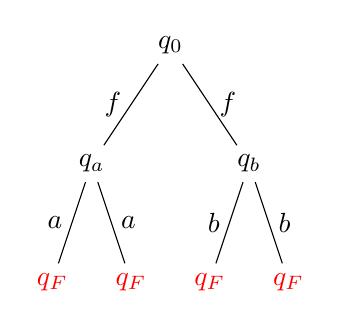
\begin{tikzpicture}
  [level 1/.style={sibling distance=2cm},
  level 2/.style={sibling distance=1cm}]
  \node {$q_0$}
    child{
      node {$q_a$}
      child{node {\color{red}$q_F$} edge from parent node[left] {$a$}}
      child{node {\color{red}$q_F$} edge from parent node[right] {$a$}}
      edge from parent node[left] {$f$}
    }
    child{
      node {$q_b$}
      child{node {\color{red}$q_F$} edge from parent node[left] {$b$}}
      child{node {\color{red}$q_F$} edge from parent node[right] {$b$}}
      edge from parent node[right] {$f$}
    };
\end{tikzpicture}

  \end{center}
  This type of tree can't be recognized by any deterministic \emph{top-down} tree automata.
  However, in the finite case, there exists deterministic \emph{bottom-up} automata, where the transition function $\d$ is reversed respectively to top-down ($Q \times Q \times A \times Q$), which are equally expressive as non-deterministic top-down automata.
\end{exercise*}

\begin{definition*}[Regular tree]
  An infinite tree $t \in \Twa$ is said to be \textbf{regular} if there are only finitely many distinct subtrees in $t$.
\end{definition*}

\begin{theorem*}[Rabin\footnotemark]
  \begin{enumerate}
    \item Any non-empty Rabin recognizable set of trees contains a regular tree.
    \item The emptiness problem for Rabin tree automata is decidable.
  \end{enumerate}
\end{theorem*}
\footnotetext{Counterpart of \Buchi theorem for trees, proved by Rabin.}

\begin{proposition*}[Rabin-tree complementation closure]
  For any non-deterministic Rabin tree automaton $\A$, there exists a Rabin tree automaton $\A'$ that recognizes the complement language $\Twa \setminus T(\A)$, \ie, Rabin tree automata are closed under complementation.
\end{proposition*}

\begin{theorem*}[S2S definability]
  A set $T \subseteq \Twa$ is definable in S2S iff it's Rabin recognizable.
\end{theorem*}

\begin{theorem*}[S2S decidability]
  The monadic second-order theory of two-successors, \ie, the set of sentences of S2S which captures those properties that are true on the binary infinite tree, is decidable.
\end{theorem*}

Recalling the tree $T_0$ from \autoref{ex:tree_t0}, we're going to show how to define it in S2S.

First, we encode the alphabet $A = \set{a,b}$ by mapping $a$ into $0$, and $b$ into $1$, like so:
\begin{center}
  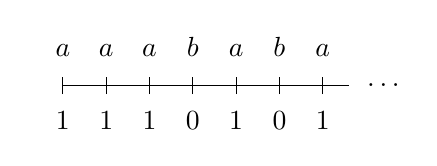
\begin{tikzpicture}[>=stealth, scale=1.1]
  \draw[-] (0,0) -- (3.3,0);
  \foreach \x in {0,0.5,1,1.5,2,2.5,3} {
    \draw (\x,-0.1) -- (\x,0.1);
  }
  \node at (-0.3,0) {$\e$};
  \node at (3.7,0) {$\dots$};
  
  \foreach \x in {0,0.5,1,2,3} {
    \node at (\x,0.4) {$a$};
    \node at (\x,-0.4) {$1$};
  }
  \foreach \x in {1.5,2.5} {
    \node at (\x,0.45) {$b$};
    \node at (\x,-0.4) {$0$};
  }
\end{tikzpicture}

\end{center}
Then we create a second-order variable $X_1$ which captures the position of the nodes in the infinite path where the $1$ occurs, and a formula $\p (X_1)$ that ensures that there exists a path with infinite many occurrences of an $a$, which is equal to:
\begin{equation*}
  \p (X_1) = \exists Y\, \Bigtuple{\text{path}(Y) \land \forall x\, \bigtuple{x \in Y \to \exists y\, \tuple{y \in Y \land x<y \land y \in X_1}}}
\end{equation*}

\begin{theorem*}
  A set $T \subseteq \Twa$ is definable in WS2S iff $T$ and its complement $\Twa \setminus T$ are \Buchi-tree recognizable.
  \vspace{-15pt}
  \begin{center}
    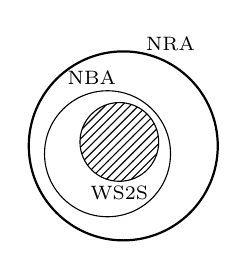
\begin{tikzpicture}
  \draw[thick] (0,0) circle (1.2);
  \draw (-0.2,-0.1) circle (0.8);
  \draw[pattern=north east lines, pattern color=black] (-0.05,0.05) circle (0.5);
  
  \node at (0.6,1.3) {\scriptsize NRA};
  \node at (-0.4,0.86) {\scriptsize NBA};
  \node at (-0.05,-0.6) {\scriptsize WS2S};
\end{tikzpicture}

  \end{center}
\end{theorem*}

\chapter{Temporal Logics}

S1S can already define every \wreg property, so why introduce yet another specification language? Because deciding S1S is \emph{non-elementary}, and its formulas -- with explicit quantification over positions and sets -- are awkward to write and read. Temporal logics keep the expressive power we need in practice while replacing position arithmetic with a handful of intuitive ``tense'' operators (\emph{next}, \emph{until}, \emph{always}, \emph{eventually}). The exact trade-off is pinned down by Kamp's theorem, stated below: LTL is precisely the \emph{first-order} fragment of S1S. These logics are the input that the model-checking algorithms of the next chapter consume.

Temporal logics are standard languages that have been introduced to resemble natural language, in order to compute formal verification of systems' properties as well as to perform model checking of systems.
Temporal logics are a special case of \textbf{modal logic}, which is an extension of propositional logic.
Modal logic differentiate from propositional logic, because, instead of having only one possible interpretation for each formula, which can be \true or \false depending on the assignment, we can have multiple interpretations depending on the \textbf{world} in which such a formula is interpreted in.
In fact, a world is set of propositions which represents its truth, \ie, makes a formula true or not.
The usefulness of this logic stands in having an accessibility relation between worlds that allows to \quoted{move} between different interpretations.
Worlds can be connected together by means of edges in a directed graph structure called \textbf{Kripke} structure.
This logic is based on two properties:
\begin{itemize}
  \item \textbf{necessity}: something must be true in \textit{all} accessible states, denoted with $\msquare$;
  \item \textbf{possibility}: something must be true in \textit{at least one} accessible states, denoted with $\Diamond$.
\end{itemize}
An example is the following:

\bigskip
\hspace{0.1\textwidth}
\begin{minipage}{0.4\textwidth}
  \begin{center}
    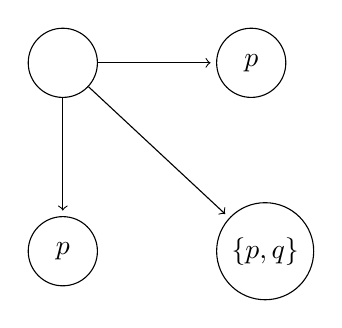
\begin{tikzpicture}[auto, node distance=1.5cm, shorten >=2pt]
  \node[state] (0) {$\emptyset$}; 
  \node[state] (p1) [right=of 0] {$\set{p}$}; 
  \node[state] (p2) [below=of 0] {$\set{p}$}; 
  \node[state] (pq) [right=of p2] {$\{p,q\}$}; 
  \path[->] 
    (0) edge (p1)
    (0) edge (p2)
    (0) edge (pq);
\end{tikzpicture}

  \end{center}
\end{minipage}
\begin{minipage}{0.4\textwidth}
  \begin{itemize}
    \item $\AP = \set{p,q}$
    \item $\msquare p$ is \true
    \item $\Diamond q$ is \true
    \item $\msquare q$ is \false
    \item $\msquare p \lor \msquare q$ is \true
  \end{itemize}
\end{minipage}

\section{Linear Temporal Logic}

Linear Temporal Logic (LTL) is a special case of Modal logic where worlds are replaced with states, which are sets of propositional letters that are supposed to hold in those states.
The Kripke structure is no more a directed graph, but is substituted with an \textbf{infinite linear order} of states, like the following:
\begin{center}
  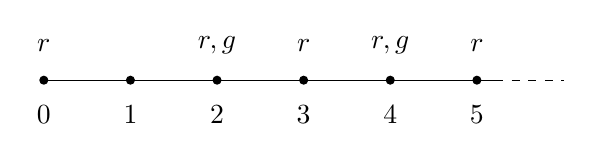
\begin{tikzpicture}[>=stealth, scale=1.1]
  \draw[-] (0,0) -- (5.3,0);
  \foreach \x in {0,1,2,3,4,5} {
    \draw[fill] (\x,0) circle (.3ex);
  }
  \draw[dashed] (5.4,0) -- (6,0);
  
  \foreach \x in {0,1,2,3,4,5} {
    \node at (\x,-0.4) {$\x$};
  }

  \node at (0,0.4) {$\set{r}$};
  \node at (1,0.4) {$\emptyset$};
  \node at (2,0.4) {$\set{r,g}$};
  \node at (3,0.4) {$\set{r}$};
  \node at (4,0.4) {$\set{r,g}$};
  \node at (5,0.4) {$\set{r}$};
\end{tikzpicture}

\end{center}
Moreover, the accessibility relation becomes a temporal ordering, where the modalities become:
\begin{itemize}
  \item \textbf{necessity}: \textit{always} in the future, denoted with $G$;
  \item \textbf{possibility}: \textit{sometimes} in the future, denoted with $F$.
\end{itemize}

\bigskip
The time representation can vary:
\begin{itemize}
  \item \emph{linear}: at each time point there is \textit{exactly one successor} and is used in LTL;
    \begin{center}
      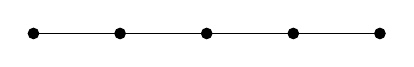
\begin{tikzpicture}[>=stealth, scale=1.1]
  \draw[-] (0,0) -- (4,0);
  \foreach \x in {0,1,2,3,4} {
    \draw[fill] (\x,0) circle (.4ex);
  }
\end{tikzpicture}

    \end{center}
  \item \emph{branching}: each time point can have \textit{multiple successors}, thus multiple futures, and is used in CTL\footnote{Computation Tree Logic};
    \begin{center}
      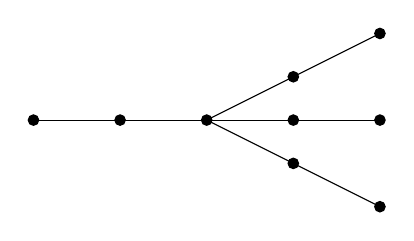
\begin{tikzpicture}[>=stealth, scale=1.1]
  \draw[-] (0,0) -- (4,0);
  \foreach \x in {0,1,2,3,4} {
    \draw[fill] (\x,0) circle (.4ex);
  }

  \draw[-] (2,0) -- (4,1);
  \draw[fill] (3,0.5) circle (.4ex);
  \draw[fill] (4,1) circle (.4ex);

  \draw[-] (2,0) -- (4,-1);
  \draw[fill] (3,-0.5) circle (.4ex);
  \draw[fill] (4,-1) circle (.4ex);
\end{tikzpicture}

    \end{center}
  \item \emph{finite}: processes eventually terminate;
    \begin{center}
      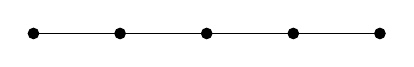
\begin{tikzpicture}[>=stealth, scale=1.1]
  \draw[-] (0,0) -- (4,0);
  \foreach \x in {0,1,2,3,4} {
    \draw[fill] (\x,0) circle (.4ex);
  }
\end{tikzpicture}

    \end{center}
  \item \emph{infinite}: computation never stops unless manual user termination;
    \begin{center}
      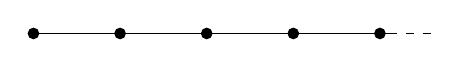
\begin{tikzpicture}[>=stealth, scale=1.1]
  \draw[-] (0,0) -- (4.2,0);
  \foreach \x in {0,1,2,3,4} {
    \draw[fill] (\x,0) circle (.4ex);
  }
  \draw[dashed] (4.3,0) -- (4.6,0);
\end{tikzpicture}

    \end{center}
  \item \emph{qualitative}: we can reason only about the order of the events;
  \item \emph{real-time}: each state is associated to a precise timestamp;
  \item \emph{discrete}: work over natural numbers;
    \begin{center}
      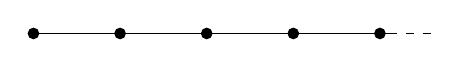
\begin{tikzpicture}[>=stealth, scale=1.1]
  \draw[-] (0,0) -- (4.2,0);
  \foreach \x in {0,1,2,3,4} {
    \draw[fill] (\x,0) circle (.4ex);
  }
  \draw[dashed] (4.3,0) -- (4.6,0);
\end{tikzpicture}

    \end{center}
  \item \emph{dense}: work over real numbers;
    \begin{center}
      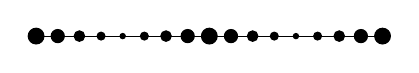
\begin{tikzpicture}[>=stealth, scale=1.1]
  \draw[-] (0,0) -- (4,0);
  \foreach \x in {0,2,4} {
    \draw[fill] (\x,0) circle (.6ex);
  }
  \foreach \x in {0.25,1.75,2.25,3.75} {
    \draw[fill] (\x,0) circle (.5ex);
  }
  \foreach \x in {0.5,1.5,2.5,3.5} {
    \draw[fill] (\x,0) circle (.4ex);
  }
  \foreach \x in {0.75,1.25,2.75,3.25} {
    \draw[fill] (\x,0) circle (.3ex);
  }
  \foreach \x in {1,3} {
    \draw[fill] (\x,0) circle (.2ex);
  }
\end{tikzpicture}

    \end{center}
  \item \emph{points};
  \item \emph{intervals}.
\end{itemize}
\begin{note}
  Notice that the past is always finite, because we assume that there is always a starting point.
\end{note}

Temporal Logics can also be distinguished by their ability to move:
\begin{itemize}
  \item \emph{pure-future/future-only}: have only the ability of moving forward in the future;
  \item \emph{past-future}: can both move backwards (finite) and forward (infinite).
\end{itemize}

Lastly, temporal logics can be distinguished by the labels:
\begin{itemize}
  \item \emph{propositional}: labels are sets of proposition letters;
  \item \emph{First-Order}: labels are an arbitrary first-order theory;
\end{itemize}

In our case, the logic we will focus on will be: linear, discrete, qualitative, infinite, future-only and propositional.

\begin{note}
  $\top$ (top) is the logic symbol for \true, while $\bot$ (bottom) for \false.
\end{note}

\begin{definition*}[Linear Temporal Logic]
  Let $\A\P = \set{p,q,r,\ldots}$ be a set of atomic propositions; the syntax of LTL is defined as follows:
  \begin{itemize}
    \item $p \mid \neg\p \mid \p \lor \p$ are the Boolean modalities
    \item $X\p \mid \p U \p$ are the Future Temporal modalities
  \end{itemize}
  where $X\p$ is the \textbf{next} operator (also denoted with $\mcirc$), which means that the formula holds at the next point in time, while $\p_1 U \p_2$ is the \textbf{until} operator, whose meaning is that $\p_1$ holds until $\p_2$ is met (we don't know when but we know it will occur).
\end{definition*}
From this basic operators, the following two function can be derived:
\begin{itemize}
  \item \textbf{eventually}: is equal to $\top\, U\, \p$ and shortly denoted with $F \p$ (also denoted with $\Diamond$).

    It means that there exists a point in time where $\p$ holds, thus corresponds to the existential quantifier;
  \item \textbf{globally}: is equal to $\neg(F\, \neg\p)$ and shortly denoted with $G \p$ (also denoted with $\msquare$).

    It means that $\p$ holds for all the points in the future, which corresponds to the universal quantifier.
\end{itemize}
The composition of the two leads to:
\begin{itemize}
  \item $GF\, \p$, which means that there are infinitely many positions where $\p$ is true;
  \item $FG\, \p$, which means that sooner or later $\p$ will be true forever (stability);
\end{itemize}

\begin{example*}
  Given $\AP = \set{p,q}$ and the formula $GF(p)$, which of the following states sequences models the formula?
  \begin{align*}
    &\set{p} \cdot \set{q} \cdot \set{p} \cdot (\set{q})^\w  &\false \\
    &(\set{p,q})^\w &\true \\
    &(\set{q} \cdot \set{q} \cdot \set{p} \cdot \set{q})^\w &\true \\
    &(\set{p})^* \cdot (\set{q})^\w &\false
  \end{align*}
  The same question, but for the formula $FG(q)$:
  \begin{align*}
    &\set{p} \cdot \set{q} \cdot \set{p} \cdot (\set{q})^\w &\true \\
    &(\set{p,q})^\w &\true \\
    &(\set{q} \cdot \set{q} \cdot \set{p} \cdot \set{q})^\w &\false \\
    &(\set{p})^* \cdot (\set{q})^\w &\true
  \end{align*}

  \bigskip
  Now are given $\AP = \set{r,g}$ and the formula $G(r \to F(g))$, which meaning is that each request $r$ is eventually followed by a grant $g$.
  As in the previous examples, which of the following states sequences models the formula?
  \begin{align*}
    &(\emptyset)^\w &\true \\
    &\set{r} \cdot \set{r} \cdot \set{r} \cdot (\emptyset)^\w &\false \\
    &\set{r} \cdot \set{r} \cdot \set{r} \cdot \set{g} \cdot (\emptyset)^\w &\true \\
    &(\set{r} \cdot \emptyset \cdot \emptyset \cdot \set{g})^\w &\true
  \end{align*}
\end{example*}

Any LTL formula is defined over a set of atomic propositions $\AP$ and interpreted over infinite words that belongs to $(2^{\AP})^\w$.
Until now we worked over $\S^\w$, so essentially here we have $\S=2^{\AP}$, where $2^{\AP}$ is the power-set of atomic propositions.

Any infinite word $\s = \tuplev{\s_0, \s_1, \ldots}$, where $\s_i \subseteq \AP$, is called a \textbf{state} and contains the atomic propositions ($\s_i$) that should hold in that state.

Moreover, sequences that belong to $(2^{\AP})^\w$ are also called state sequences or \textbf{traces}.
An example is the following:
\begin{figure}[H]
  \hspace{0.05\textwidth}
  \begin{minipage}{0.45\textwidth}
    \begin{center}
      $\AP = \set{r,g}$
    \end{center}
  \end{minipage}
  \begin{minipage}{0.45\textwidth}
    \begin{center}
      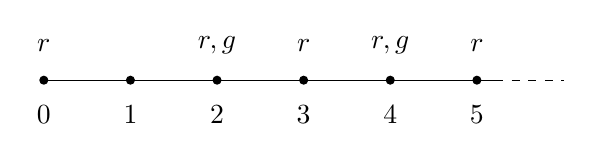
\begin{tikzpicture}[>=stealth, scale=1.1]
  \draw[-] (0,0) -- (5.3,0);
  \foreach \x in {0,1,2,3,4,5} {
    \draw[fill] (\x,0) circle (.3ex);
  }
  \draw[dashed] (5.4,0) -- (6,0);
  
  \foreach \x in {0,1,2,3,4,5} {
    \node at (\x,-0.4) {$\x$};
  }

  \node at (0,0.4) {$\set{r}$};
  \node at (1,0.4) {$\emptyset$};
  \node at (2,0.4) {$\set{r,g}$};
  \node at (3,0.4) {$\set{r}$};
  \node at (4,0.4) {$\set{r,g}$};
  \node at (5,0.4) {$\set{r}$};
\end{tikzpicture}

    \end{center}
  \end{minipage}
\end{figure}

\subsubsection{Satisfiability}

We denote with $\s,i \models \p$ when an LTL formula $\p$ is satisfied by a state $\s$ at position $i$.
Satisfiability for LTL modalities is defined as follows:
\begin{itemize}
  \item base case, $p$ holds at position $i$:
    \begin{equation*}
      \s,i \models p \ \iff\  p \in \s_i
    \end{equation*}
  \item negation, $\p$ doesn't hold at position $i$:
    \begin{equation*}
      \s,i \models \neg\p \ \iff\  \s,i \not\models \p
    \end{equation*}
  \item conjunction, $\p_1$ and $\p_2$ hold at position $i$:
    \begin{equation*}
      \s,i \models \p_1 \land \p_2 \ \iff\  \s,i \models \p_1 \,\land\, \s,i \models \p_2
    \end{equation*}
  \item next operator, $\p$ holds at the next position of $i$:
    \begin{equation*}
      \s,i \models X\p \ \iff\ \s,i+1 \models \p
    \end{equation*}
  \item until operator, $\p_1$ holds until $\p_2$ holds:
    \begin{equation*}
      \s,i \models \p_1 U \p_2 \ \iff\ \exists j \ge i \ \Big(\s,j \models \p_2 \,\land\, (\forall k\ \, \s,k \models \p_1 \text{ with } i \leq k < j)\Big)
    \end{equation*}
    and there exists also a strict version, denoted with $U^S$, without equals.
\end{itemize}
In particular, we say that $\s$ is a \textbf{model} of $\p$, if satisfies it from position 0, \ie
\begin{equation*}
  \s \models \p \ \iff\  \s,0 \models \p
\end{equation*}

\bigskip
The \textbf{language} of LTL formula $\p$ is\
\begin{equation*}
  \L(\p) = \set{\s \in \sAP \mid \s \models \p}
\end{equation*}
and we say that $\p$ is \emph{satisfiable} iff $\L(\p) \neq \emptyset$ and that is \emph{valid} when $\L(\p) = \sAP$.

\begin{example*}
  Considering $\AP = \set{p,q}$, which of the following states sequences models the given formulas?
  \begin{displaybox}
    \begin{center}
      \begin{tabular}{l|c|c|c} 
        & $F(p) \land F(q)$ & $F\big(p \land F(q)\big)$ & $F(p \land q)$ \\
        \hline
        $(\emptyset)^\w$ & \false & \false & \false \\
        $(\emptyset)^* \cdot \set{q} \cdot \emptyset \cdot \set{p} \cdot (\emptyset)^\w$ & \true & \false & \false \\
        $(\emptyset)^* \cdot \set{p} \cdot \emptyset \cdot \set{q} \cdot (\emptyset)^\w$ & \true & \true & \false \\
        $(\emptyset)^* \cdot \set{p,q} \cdot (\emptyset)^\w$ & \true & \true & \true
      \end{tabular}
    \end{center}
  \end{displaybox}
\end{example*}

\begin{example*}
  Considering $\AP = \set{p,q}$ and the LTL formula $p\, U\, (G\, q)$ the equivalent \wreg expression is
  \begin{equation*}
    p^* \cdot (pq \cup q)^\w
  \end{equation*}
  Here each symbol denotes \emph{any} state satisfying it (so $p$ stands for $\set{\set{p},\set{p,q}}$ and $q$ for $\set{\set{q},\set{p,q}}$); under this reading $pq \cup q = q$, \ie, the prefix keeps $p$ true and the suffix keeps $q$ true forever.
  With the exact-letter convention used elsewhere (where $p$ means literally the letter $\set{p}$) the faithful expression is instead $(p \cup pq)^* \cdot (q \cup pq)^\w$.
\end{example*}

\begin{example*}
  Considering $\AP = \set{p,q}$, is the formula $FX\, p$ equivalent to $XF\, p$?

  Yes, because the first implies to have a position for which in the next $p$ holds, and the next position will eventually hold for $p$.

  \bigskip
  And the formula $(G\, p)\, U\, q$ is equivalent to $p\, U\, q$?
  No, in fact the first is stricter than the second.
  That's because the first implies that $p$ must hold for hold from the starting position until reaching $q$, while the second requires $p$ to hold only when $q$ occurs, thus $p$ should not have to be always true before $q$.
\end{example*}

\subsubsection{Fairness constraints}

The \textbf{compassion} constraint implies that it's not possible that a transition is enabled infinitely many times, but taken only finitely many.
This constraint can be express in LTL with the following expression:
\begin{equation*}
  \neg\Big( GF(\text{enabled}) \land FG(\neg\text{taken})\Big)
\end{equation*}
or more simply $GF(\text{enabled}) \to GF(\text{taken})$, \ie, if a transition is enabled infinitely many times, then it must also be taken infinitely many times.
\begin{note}
  Notice that $GF(\text{enabled} \to \text{taken})$ is not equal to the above, because requires the transition to be taken at the same time it's enabled, which is a much stricter requirement.
\end{note}

\bigskip
The \textbf{justice} constraint requires that it never occurs that a transition is always enabled and never taken.
The correspondent LTL expression is:
\begin{equation*}
  \neg F \Big( G(\text{enabled}) \land G(\neg\text{taken})\Big)
\end{equation*}
or shortly $G\Big(G(\text{enabled}) \to F(\text{taken})\Big)$.

\bigskip
Recall that Negation Normal Form of a formula has the negation only applied to atomic propositions. Pushing negations inward through the temporal operators needs a \emph{dual} for each one: \quoted{next} is self-dual, but \quoted{until} has no syntactic dual among the operators above. Its dual is the \textbf{release} operator $\p_1 \RRR \p_2 \equiv \neg(\neg\p_1 \UU \neg\p_2)$ (\quoted{$\p_2$ holds until $\p_1$ releases it, or holds forever}); we meet it again as the greatest-fixpoint companion of \emph{until} in CTL model checking.

\begin{theorem*}[Kamp]
  For each LTL formula $\p$, there exists an S1S first-order formula $\psi$ \st $\L(\p) = \L(\psi)$, and vice versa.
\end{theorem*}

This theorem proves how LTL captures only partially S1S, in particular, only first-order formulas.

\subsection{Tableaux for LTL}

Tableaux have two methods for representing the accessibility relation:
\begin{itemize}
  \item \emph{implicit}: the accessibility relation is built in tableaux's structure and this is used with linear/branching temporal logic;
  \item \emph{explicit}: is kept track of the accessibility relation via a separate structure from the tableau, and it's used with interval temporal logics.
\end{itemize}
plus there are two different methods to compute formulas:
\begin{itemize}
  \item \emph{declarative}: works over all possible sets of sub-formulas and search for at least one valid path;
  \item \emph{incremental}: works over only the \quoted{meaningful} set of sub-formulas generating them when needed, which makes the performance more efficient.
\end{itemize}

\begin{definition}[Closure of $\p$]\label{def:closure_phi}
  The smallest set of sub-formulas of a formula $\p$ is called \textbf{closure} $\phi_\p$ and is defined as follows:
  \begin{itemize}
    \item $\p \in \phi_\p$;
    \item for every formula/sub-formula $p$ in $\phi_p$, also all its sub-formulas $q$ its negation $\neg p$ belong to $\phi_p$;
    \item every formula $\psi$ of the form $G\, p,\ F\, p,\ p\,U\,q$ that belongs to $\phi_\p$ implies that also $X \psi$ belongs to $\phi_\p$.
  \end{itemize}
\end{definition}

Because we have to take into account temporality of formulas, the expansion rules for tableaux over temporal logic are the followings:
\begin{itemize}
  \item $G p \approx p \land XG p$
  \item $F p \approx p \land XF p$
  \item $p\,U\,q \approx q \lor \big(p \land X(p\,U\,q) \big)$
\end{itemize}
which means that if they're not true in that position, then they will be true in the following (next operator), allowing an infinite expansion to not lose track of the evolution of time while expanding the other formulas into sub-formulas.
The last condition of the closure $\phi_\p$ has been added to take into account these expansions.

We can distinguish between two types of formulas:
\begin{itemize}
  \item $\a$: all those formulas that are a conjunction of sub-formulas, \ie, $p \land q$ and $Gp$.
    These expand into a single comma-separated formula, where all the sub-formulas must be true to make the original $\a$ formula true, \ie,
    \begin{center}
      \begin{tabular}{l|c} 
        $\a$ & $k(\a)$ \\
        \hline
        $p \land q$ & $p,q$ \\
        $Gp$ & $p,XGp$
      \end{tabular}
    \end{center}
  \item $\b$: all those formulas that are a disjunction of sub-formulas, \ie, $p \lor q$, $Fp$ and $p \,U\, q$.
    Oppositely to the $\a$ ones, each sub-formula becomes and individual formula, thus just one of these sub-formulas is needed to make the original $\b$ formula true, \ie,
    \begin{center}
      \begin{tabular}{l|c|c} 
        $\b$ & $k_1(\b)$ & $k_2(\b)$ \\
        \hline
        $p \lor q$ & $p$ & $q$ \\
        $Fp$ & $p$ & $XFp$ \\
        $p \,U\, q$ & $q$ & $p \land X(p \,U\, q)$
      \end{tabular}
    \end{center}
\end{itemize}

\begin{definition}[$\p$-atom]\label{def:p_atom}
  An atom $A$ over $\p$ and is a set of sub-formulas of $\phi_\p$, that satisfies the following conditions:
  \begin{itemize}
    \item the conjunction of the sub-formulas in the atom is satisfiable, \ie, at least one of the sub-formulas is \true;
    \item each atom can contain only a sub-formula $p$ or it's negation $\neg p$, not both, \ie, $p$ and $\neg p$ must belong to different atoms;
    \item lastly, if an atom has an $\a$ formula, all its sub-formulas must be in the atom, while for $\b$ formulas, its necessary that at least one of its sub-formulas belongs to the atom.
  \end{itemize}
\end{definition}

Tableau is a type of graph where nodes are associated atoms.
Nodes are connected together via directed edges and represents the expansion of a formula in the atom.
Moreover, if exists is at least one path through the nodes in the tableau that is satisfiable, it means that there exists at least a state sequence that models the formula $\p$.
For this reason, we can say that each atom represent the maximal mutually-satisfiable set of formulas, where a set is mutually-satisfiable if exists a model and a position such that every formula in the set holds for them.

\begin{definition*}[Basic formula]
  A \textbf{basic formula} is a proposition or a formula of the form $Xp$.
\end{definition*}

The presence/absence of a basic formula in an atom, determines the presence/absence of the closure formulas relative to it.
For example, supposing that we have $XGp$ in an atom, it implies that either $p \ort \neg p$ must be in that atom.
\begin{figure}[H]
  \centering
  \begin{tikzpicture}
  [level 1/.style={sibling distance=3cm},
  level 2/.style={sibling distance=1cm}]
  \node {$\p = q \lor Gp$}
      child {
          node {$q$}
      }
      child {
          node {$Gp$}
          child { node {$p,XG p$} }
      };
\end{tikzpicture}

  \caption{Example of LTL tableau}
\end{figure}

\begin{definition*}[Induced path]
  Given a model $\s$ of a formula $\p$, we say that an infinite path\footnote{An infinite sequence of atoms $A_0 A_1 \ldots$} $\pi_\s$ in the tableau for $\p$ ($T_\p$) is \textbf{induced} by $\s$ if it holds that
  \begin{equation*}
    \forall p \in \phi_\p, i \ge 0 \qquad \s,i \models p
  \end{equation*}
  where $p$ belongs to one of the atoms in the infinite path.
\end{definition*}
Form this definition it follows that, a tableau for $\p$ will contain for sure all the correct models of $\p$, but at the same time it doesn't mean that it contains only them, in fact it can contain also incorrect ones.

\begin{definition*}[Promise]
  A formula $\psi$ \textbf{promises} a formula $r$ if $\psi$ is in the form $Fr, \neg G \neg r \ort p \,U\, r$.

  \bigskip
  They properties of this promise are:
  \begin{itemize}
    \item if $\s,i \models \psi$, then $\s,j \models r$ for some $j \ge i$;
    \item the model $\s$ contains infinite-many positions $i \ge 0$ \st $\s,i \models \neg \psi \ort \s,i \models r$.
  \end{itemize}
\end{definition*}

\begin{definition*}[Fulfillment]
  An \textit{atom} $A$ \textbf{fulfills} a formula $\psi$ that promises $r$ if either $\neg \psi \ort r$ belongs to $A$.

  \bigskip
  A \textit{path} $\pi$ is fulfilling if for each promising formula $\psi$, it contains infinitely many atoms that fulfill each $\psi$.
  Moreover, if a path $\pi_\s$ is induced by a model $\s$, then $\pi_\s$ is fulfilling and vice versa, explicitly, if $\pi$ is a fulfilling path, then there exists a model $\s$ that induces $\pi$, thus $\pi = \pi_\s$.
\end{definition*}

\begin{definition*}[Satisfiability]
  A formula $\p$ is satisfiable iff its tableau $T_\p$ contains a fulfilling path $\pi = A_0,A_1,\ldots$ \st $\p$ belongs in the first atom $A_0$, \ie, the path starts from $\p$.
\end{definition*}

\begin{question*}[Is $\p = Gp \land F \neg p$ satisfiable?]
  To check its satisfiability, we must check if the corresponding tableau $T_\p$ contains a fulfilling path that starts with $\p$.
  \begin{center}
    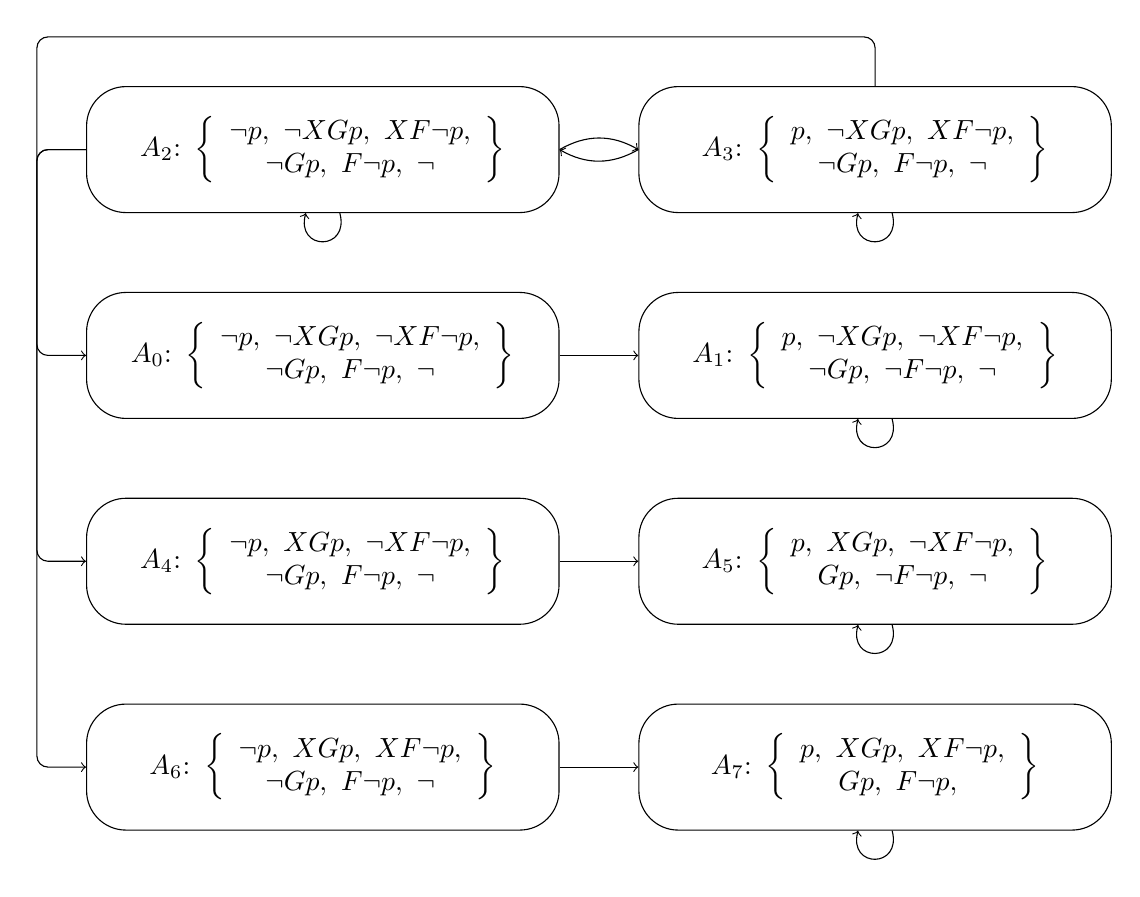
\begin{tikzpicture}[
    state/.style={draw,rectangle,rounded corners=0.5cm,minimum width=6cm,minimum height=1.6cm,align=center},
]

  \node[state] (A2) {$A_2{:}\ \left\{\begin{array}{c} \neg p,\ \neg XGp,\ XF\neg p,\\ \neg Gp,\ F\neg p,\ \neg \p\end{array}\right\}$};
  \node[state, right=of A2] (A3) {$A_3{:}\ \left\{\begin{array}{c} p,\ \neg XGp,\ XF\neg p,\\ \neg Gp,\ F\neg p,\ \neg \p\end{array}\right\}$};
  \node[state, below=of A2] (A0) {$A_0{:}\ \left\{\begin{array}{c} \neg p,\ \neg XGp,\ \neg XF\neg p,\\ \neg Gp,\ F\neg p,\ \neg \p\end{array}\right\}$};
  \node[state, right=of A0] (A1) {$A_1{:}\ \left\{\begin{array}{c} p,\ \neg XGp,\ \neg XF\neg p,\\ \neg Gp,\ \neg F\neg p,\ \neg \p\end{array}\right\}$};
  \node[state, below=of A0] (A4) {$A_4{:}\ \left\{\begin{array}{c} \neg p,\ XGp,\ \neg XF\neg p,\\ \neg Gp,\ F\neg p,\ \neg \p\end{array}\right\}$};
  \node[state, right=of A4] (A5) {$A_5{:}\ \left\{\begin{array}{c} p,\ XGp,\ \neg XF\neg p,\\ Gp,\ \neg F\neg p,\ \neg \p\end{array}\right\}$};
  \node[state, below=of A4] (A6) {$A_6{:}\ \left\{\begin{array}{c} \neg p,\ XGp,\ XF\neg p,\\ \neg Gp,\ F\neg p,\ \neg \p \end{array}\right\}$};
  \node[state, right=of A6] (A7) {$A_7{:}\ \left\{\begin{array}{c} p,\ XGp,\ XF\neg p,\\ Gp,\ F\neg p,\ \p\end{array}\right\}$};

  \node[above=0.5 of A2] (x0) {};
  \node[left=0.5 of A2] (x1) {};
  \node[above left=0.5cm and 0.5cm of A0] (a0) {};
  \node[above left=0.5cm and 0.5cm of A4] (a4) {};
  \node[above left=0.5cm and 0.5cm of A6] (a6) {};

  \path[->]
    (A2.east) edge[bend left] (A3.west)
    (A3.west) edge[bend left] (A2.east)
    (A0) edge (A1)
    (A4) edge (A5)
    (A6) edge (A7);
  
  \path[->]
    (A2) edge[loop below,distance=0.5cm] (A2)
    (A3) edge[loop below,distance=0.5cm] (A3)
    (A1) edge[loop below,distance=0.5cm] (A1)
    (A5) edge[loop below,distance=0.5cm] (A5)
    (A7) edge[loop below,distance=0.5cm] (A7);

  \draw[->,rounded corners] (A3.north) |- (x0.west) -- (x0.east) -| (x1.south) -- (x1.north) |- (A0.west);
  \draw[->,rounded corners] (A2.west) -| (a4.south) -- (a4.north) |- (A4.west);
  \draw[->,rounded corners] (A2.west) -| (a6.south) -- (a6.north) |- (A6.west);

\end{tikzpicture}

  \end{center}
  From the built tableau, it's immediate to see that only the atom $A_7$ has $\p$, but it's not a fulfilling path because can only loop in itself and thus $F\neg p$ can't be satisfied, because we have $p$ and in any future we can't have $\neg p$.
  For this reason $\pi$ isn't satisfiable.
\end{question*}

An easier approach to check on the existence of fulfilling paths starting at $\p$ is to use strongly connected subgraphs.

\begin{definition*}[Strongly Connected Subgraph]
  A subgraph $S$ of a tableau $T_\p$ is said to be a \textbf{Strongly Connected Subgraph} (SCS) if for all pairs of atoms in $S$ there exists a path that connects them only through atoms of $S$.

  \bigskip
  Moreover, $S$ is
  \begin{itemize}
    \item \emph{fulfilling}: if it's \textit{non-transient}\footnote{A \textit{transient} node is a node not connected to itself, but has only incoming/outgoing edges to other nodes, like $A_0,A_4 \andt A_6$ of the tableau in the previous question. \textit{Non-transient} is the opposite.} and if every formula $\psi$ that promises $r$ is fulfilled by some atom in $S$;
    \item \emph{$\p$-reachable}: if exists a finite path that starts with $\p$ and the last atom of the path belongs to $S$;
    \item \emph{maximal} (MSCS): if it's not contained in any larger SCS (\eg, $A_2 \andt A_3$).
      Any MSCS is also \emph{terminal} if there are no atoms of $S$ connected to other atoms \textit{not} belonging to $S$ (\eg, $A_5 \andt A_7$).
  \end{itemize}
\end{definition*}

\begin{proposition*}
  A tableau $T_\p$ contains a fulfilling path that starts from a $\p$-atom iff it contains a $\p$-reachable SCS.
\end{proposition*}

\begin{proposition*}
  A formula $\p$ is satisfiable iff its tableau $T_\p$ contains a $\p$-reachable fulfilling MSCS.
\end{proposition*}

Following these propositions, a \textbf{pruning criterion} to reduce the size of a tableau consists in removing all its parts that don't respect these propositions, \ie, that a priori we know they don't satisfy the formula.
In particular, we can remove any MSCS not reachable from a $\p$-atom, plus any terminal MSCS that is not fulfilling.
Any MSCS that's not fulfilling but it's also \textit{not} terminal must not be removed because can be part of a path that leads to another MSCS which may be fulfilling.

\bigskip
Using the same approach for satisfiability, we can check for \textbf{validity} of a formula $\p$, by checking for satisfiability of $\neg \p$.
Trivially, if it's satisfiable, it means that $\p$ it's not valid.

\subsection{Linear Temporal Logic with Past}

Abbreviated to LTL+P, extends LTL by adding \textbf{past} temporal modalities, which are:
\begin{itemize}
  \item $Y\p$ is the \textbf{Yesterday} operator and works oppositely to the next operator, in fact its meaning is that $\p$ holds at the previous time position (if there is any);
  \item $\p_1 S \p_2$ is the \textbf{Since} operator and is the opposite of the until one, and means that there exists a position in the past where $\p_2$ was true and $\p_1$ holds from that point ongoing.
\end{itemize}
Satisfiability of these past modalities is defined as follows:
\begin{itemize}
  \item yesterday operator, $\p$ holds at the previous position of $i$ if exists a predecessor of $i$:
    \begin{equation*}
      \s,i \models Y\p \ \iff\ i>0 \land \s,i-1 \models \p
    \end{equation*}
    Note that $\s,0 \models Y\p$ is always \false.
  \item since operator, $\p_1$ holds since $\p_2$ held:
    \begin{equation*}
      \s,i \models \p_1 S \p_2 \ \iff\ \exists j \leq i \ \Big(\s,j \models \p_2 \,\land\, (\forall k\ \, \s,k \models \p_1 \text{ with } j < k \leq i)\Big)
    \end{equation*}
\end{itemize}
Like in plain LTL, can be constructed some shortcuts with the past temporal operators, which are:
\begin{itemize}
  \item $\wY \p$ is the \textbf{weak Yesterday} operator, which means that $\p$ holds at the previous position (doesn't matter if there is no previous position, \ie, predecessor). In fact $\wY \p \equiv \neg Y\, \neg\p$. Note that $\s,i \models \wY \bot$ holds only for $i = 0$;
  \item $O \p$ is the \textbf{Once} operator, opposite of the eventually, and means that there exists a time in the past where $\p$ holds, \ie, $O \p \equiv \true\, S\, \p$;
  \item $H \p$ is the \textbf{Historically} operator, opposite of the globally, and means that at all time points in the past $\p$ holds, \ie, $H \p \equiv \neg(O\, \neg\p)$.
\end{itemize}

\begin{theorem*}
  LTL+P is as expressive as LTL.
\end{theorem*}
This proves that past operators do not make any difference in the type and number of languages that can be recognized by this logic.

For simplicity, we will denote with $\p \in $ LTL to denote that $\p$ is a formula of LTL, and with $\abs{\p}$ the size of its tableau tree.

\begin{definition*}[Extended closure of $\p$]
  The extended closure of $\p$ is denoted with $\C(\p)$ and is defined as the \nameref{def:closure_phi} ($\phi_\p$), but with this additional property for the past operators:
  \begin{itemize}
    \item every formula $\psi \in \C(\p)$ of the form $p\,S\,q$ implies that also $Y \psi \andt \wY \psi$ belongs to the extended closure $\C(\p)$.
  \end{itemize}
\end{definition*}

To solve LTL+P satisfiability for a formula $\p$, we can build an equivalent NBA $\A_\p$ \st $\L(\p) = \L(\A_\p)$, \ie, they recognize the same language.
Then we can check for the emptiness of $\A_\p$, which means that if $\L(\A_\p) = \emptyset$, then $\p$ is unsatisfiable, otherwise it's satisfiable.

\begin{theorem}[LTL+P succinctness]\label{thm:ltlp_succ}
  LTL+P \textit{can} be exponentially \textbf{more succinct}\footnote{shorter formula that doesn't lose on meaning} than LTL.

  \bigskip
  This is the case when exists a family of languages $\set{L_n}^\infty_{n=1} \subseteq (2^{\S_n})^\w$ \st $\forall n > 0$
  \begin{enumerate}
    \item $L_n$ is definable in LTL+P with a formula of linear size ($\mathcal{O}(n)$);
    \item $L_n$ is \textbf{not} definable in LTL with a formula of size at least exponential ($2^{\O(n)}$).
  \end{enumerate}
  where $\S_n = \set{\vars{p}{0}{n}}$ and the language $L_n$ is the set of words in which, if any position $i$ agrees with position $0$ on the interpretation of all $\vars{p}{1}{n}$, then $i$ and $0$ agree also on the interpretation of $p_0$.
\end{theorem}

\begin{proof*}[\nameref{thm:ltlp_succ}]
  \begin{enumerate}
    \item[\textcolor{pink!200}{1.}] To prove it we can define a LTL+P formula equivalent to $L_n$:
      \begin{equation*}
        G \Bigg( \Big( \bigwedge^n_{i=1} \big(\,p_i \iff \mathcal{O}(\wY\bot \land p_i)\,\big) \Big) \quad\to\quad \Big( \big(\,p_0 \iff \mathcal{O}(\wY\bot \land p_0)\,\big) \Big) \Bigg)
      \end{equation*}
    \item[\textcolor{pink!200}{2.}] We know that
      \begin{enumerate}
        \item[2.1] each LTL+P formula $\p$ can be translated into an equivalent NBA of size at most exponential in $\abs{\p}$;
        \item[2.2] any NBA over $\sAP$ that recognizes $L_n$ has size $2^{2^{\O(n)}}$.
      \end{enumerate}
      Supposing that there exist $n>0$ and a formula $\p \in $ LTL+P \st $\L(\p) = L_n$ and $\abs{\p}$ is less than exponential, then it should also exist a equivalent NBA which is at most exponential, according to point 2.1.
      However, this is a contradiction with point 2.2, because any NBA that recognizes $L_n$ must be doubly exponential in $n$.
  \end{enumerate}
\end{proof*}

\section{Computation Tree Logic}

A CTL model $M$ (a Kripke structure) is a triple $(S,R,L)$ where:
\begin{itemize}
  \item $S$ is the set of states;
  \item $R \subseteq S \times S$ is the (binary) transition relation between states;
  \item $L: S \to 2^{\AP}$ assigns to each state the set of propositional letters that hold in it.
\end{itemize}
The structure is almost the same of LTL, but the key difference stands in the language used, which allow the concurrent evaluation of multiple branches.

\begin{example*}
  An example of CTL is:
  \begin{itemize}
    \item $S = \set{q_0,q_1,q_2}$
    \item $R = \set{(q_0,q_0),(q_0,q_1),(q_1,q_2),(q_2,q_2)}$
    \item $L(q_0) = \set{p}$
    \item $L(q_1) = \emptyset$
  \end{itemize}
\end{example*}

In CTL, $\XX$ (\quoted{next}) and $\UU$ (\quoted{until}) are \textbf{temporal operators}: they build a \emph{path formula} out of state formulas. The \textbf{path quantifiers} $\AA$ (\quoted{for all futures}) and $\EE$ (\quoted{there exists a future}) then turn a path formula back into a \emph{state formula} by quantifying over the paths leaving a state.
Moreover, in this language, it's forced that path quantifiers have to be interleaved with a state quantifier, and the root of the formula tree must start with a CTL operator.
This allows model checking to be computed in polynomial time at the expenses of losing expressiveness (we don't lose in fairness).

The CTL syntax is:
\begin{itemize}
  \item each propositional letter $P \in \AP$ is a state formula;
  \item given two state formulas $p \andt q$, then $p \land q$ and $\neg p$ are state formulas as well;
  \item given a path formula $p$, then $\AA p$ and $\EE p$ are state formulas instead;
  \item given two state formulas $p \andt q$, then $\XX p$ and $p \UU q$ are path formulas.
\end{itemize}

$\AG$ is a very standard pattern that is used to express that means \quoted{for all paths and for all states in each path}, \ie, for every node in the tree.

\begin{example*}
  We consider the CTL formula $\AG(p \to \AF q)$, with $p,q \in \AP$.
  Because it's an implication, we consider only paths that have $p$ \true (if none it means that the formula is valid).
  Now we consider the subtree rooted in a node $p$ of a path and we search to satisfy $\AF q$, which means that we search if there exists a future node with $q$ in all the paths starting from $p$, because $\FF$ means \quoted{eventually}.
  \begin{center}
    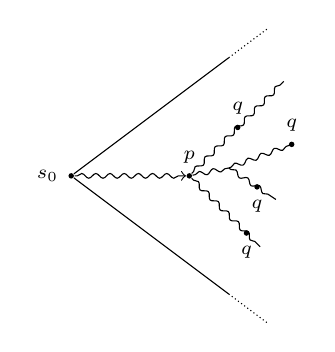
\begin{tikzpicture}[
    every node/.style={font=\scriptsize},
    snake/.style={
        decorate,
        decoration={snake,segment length=1.8mm,amplitude=0.3mm,pre length=1pt,post length=1pt}
    },
    dot/.style={
        fill,
        circle,
        inner sep=0.7pt
    }
]

\node[dot,label=left:$s_0$] (s0) at (0,0) {};

\draw (s0) -- (2,1.5);
\draw[densely dotted] (2,1.5) -- ++(0.5,0.375);
\draw (s0) -- (2,-1.5);
\draw[densely dotted] (2,-1.5) -- ++(0.5,-0.375);

\node[dot,label=above:$p$] (p) at (1.5,0) {};
\draw[->,snake] (s0) -- (p);

\draw[snake] (p) -- node[dot,pos=.5,label=above:$q$] {} (2.7,1.2);

\draw[snake] (p) -- (2,0.1);
\draw[snake] (2,0.1) -- node[dot,pos=1,label=above:$q$] {} (2.8,0.4);
\draw[snake] (2,0.1) -- node[dot,pos=.6,label=below:$q$] {} (2.6,-0.3);

\draw[snake] (p) -- node[dot,pos=.8,label=below:$q$] {} (2.4,-0.9);

\end{tikzpicture}

  \end{center}

  We consider the CTL formula $\EF q \land \EF \EG p$.
  $\EF q$ means that starting from the root there exists a future node in a path where there is $q$.
  At the same time $\EF \EG p$ must be satisfied, which means that starting from the root there exists at least one path where $\EG p$ is true, \ie, from that node onwards $p$ will be always true.
  Note that $\EF \EG p$ doesn't have to be on the same path of $\EF q$, nor that has to start from $q$, because in that case the formula would have been $\EF(q \land \EG p)$.
  \begin{center}
    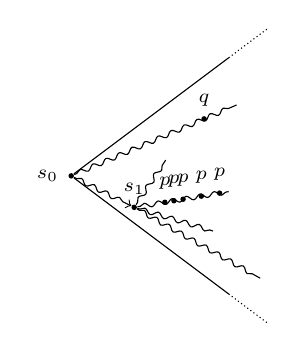
\begin{tikzpicture}[
    every node/.style={font=\scriptsize},
    snake/.style={
        decorate,
        decoration={snake,segment length=1.8mm,amplitude=0.3mm,pre length=1pt,post length=1pt}
    },
    dot/.style={
        fill,
        circle,
        inner sep=0.7pt
    }
]

\node[dot,label=left:$s_0$] (s0) at (0,0) {};

\draw (s0) -- (2,1.5);
\draw[densely dotted] (2,1.5) -- ++(0.5,0.375);
\draw (s0) -- (2,-1.5);
\draw[densely dotted] (2,-1.5) -- ++(0.5,-0.375);

\draw[snake] (s0) -- node[dot,pos=0.8,label=above:$q$] {} (2.1,0.9);

\node[dot,label=above:$s_1$] (s1) at (0.8,-0.4) {};
\draw[->,snake] (s0) -- (s1);

\draw[snake] (s1) -- (1.2,0.2);
\draw[snake] (s1) --
  node[dot,pos=.3,label=above:$p$] {}
  node[dot,pos=.4,label=above:$p$] {}
  node[dot,pos=.5,label=above:$p$] {}
  node[dot,pos=.7,label=above:$p$] {}
  node[dot,pos=.9,label=above:$p$] {}
  (2,-0.2);
\draw[snake] (s1) -- (1.8,-0.7);
\draw[snake] (s1) -- (2.4,-1.3);

\end{tikzpicture}

  \end{center}

  Lastly, if we have a formula of the form $\GG(p \to \FF q)$, this is different from $\GF p \to \GF q$.
\end{example*}

LTL is incapable of expressing possibility constraints, while CTL cannot express some fairness constraints, which is why LTL and CTL are expressively \textbf{incomparable}.
An example of an LTL formula not translatable into CTL is $\p = \FG p$, while in the opposite direction there is $\p = \AG(p \to \EF q)$.
Intuitively, LTL reasons about \emph{one path at a time}, so it cannot talk about the \emph{branching} structure -- which alternative futures exist; CTL reasons about the branching structure but cannot follow a single path arbitrarily far. Hence $\FG p$ (\quoted{on every path, eventually $p$ holds forever}) escapes CTL, while $\AG(p \to \EF q)$ (\quoted{from every reachable state, some future reaches $q$}) escapes LTL.

Some shorthand notation is:
\begin{itemize}
  \item $\EF \a = \EU(\top,\a)$;
  \item $\AF \a = \AU(\top,\a)$;
  \item $\EG \a = \neg \AF \neg \a$;
  \item $\AG \a = \neg \EF \neg \a$.
\end{itemize}
These fixpoint-flavoured equivalences are not idle: they are exactly what makes CTL \emph{efficiently} checkable, and they reappear verbatim as the recursive cases of the CTL model-checking algorithm in the next chapter.

\bigskip
We can now \emph{state} what a system should do, in either the linear style (LTL) or the branching style (CTL). What we still cannot do is \emph{decide}, given a system, whether it actually behaves that way. That algorithmic question -- model checking -- is the subject of the next chapter, which also confronts the obstacle that makes it hard in practice: the sheer number of states.

\chapter{Model Checking}

Formal methods are a set of techniques to mathematically specify and verify systems, and model checking is one type of formal method.
Model checking it's the most used and its distinctive features are:
\begin{itemize}
  \item fully automatic;
  \item exhaustive;
  \item not biased to the most possible scenario unlike testing;
  \item generates a counterexample trace when specifications fail to hold.
\end{itemize}

The downsides of model checking are essentially:
\begin{itemize}
  \item is less data-oriented;
  \item can be only as good as the model is;
  \item doesn't have any guarantees about returning a complete result.
\end{itemize}

The model checking process is divided in the following phases:
\begin{enumerate}
  \item modeling: the system is formalized;
  \item running: is executed the checker;
  \item analysis: check of the output to see if the properties are satisfied or the computation stopped due to out of memory.
\end{enumerate}

The link back to the earlier chapters is this. The set of all computations of a system is an $\w$-language; a temporal specification $\p$ defines another $\w$-language $\L(\p)$; and ``the system satisfies $\p$'' means the first language is \emph{contained} in the second. By complementation this is an \emph{emptiness} test on the intersection of the system with an automaton for $\neg\p$ -- exactly the $\w$-automata machinery of Chapter~\ref{cha:automata}. The two algorithms below (for LTL and CTL) are concrete instances of this idea, and the later sections make it scale.

\section{Kripke Structures}

Both algorithms in this chapter take their model to be a Kripke structure: a finite, fully-labelled transition graph. It is the explicit-state specialisation of the Fair Transition Systems of Chapter~\ref{cha:automata} -- the states are now finitely many and labelled by propositions -- and it is the structure over which LTL and CTL are interpreted.

\begin{definition*}[Kripke structure]
  A Kripke structure, also called transition system, is a tuple $M = \tuplev{\AP,Q,I,T,L}$ where:
  \begin{itemize}
    \item $\AP$ is a finite alphabet;
    \item $Q$ is the finite set of state;
    \item $I \subseteq Q$ is the set of initial states;
    \item $T \subseteq Q \times Q$ is a complete transition relation;
    \item $L: Q \to 2^{\AP}$ is the function that assigns to each state the set of atoms in $\AP$ that are \true in that state.
  \end{itemize}
\end{definition*}

\begin{note}
  When fairness matters -- as in the LTL algorithm below, which speaks of \emph{justice} and \emph{compassion} -- this transition relation is enriched with the fairness sets $\J$ and $\C$ of a Fair Transition System (Chapter~\ref{cha:automata}). The bare Kripke structure above is the special case with no fairness requirements.
\end{note}

\section{LTL Model Checking}

Model checking of LTL is equal to check satisfiability of a finite-state program.

\begin{definition*}[Model Checking of LTL]
  Given a Kripke structure $M$, an state $s$ from the set of initial states $I$ and an LTL formula $\p$ over $\AP$, we denote with $M,s \models A\p$ when all paths of $M$ that starts from $s$ are models of $\p$, in fact $A$ means for all paths.

  In other words, the model checking problem over LTL (LTL-MC) is the problem of establishing whether $M,s \models A\p$, and its complexity is PSPACE-complete.
\end{definition*}

\begin{example*}
  Given the following Kripke structure
  \begin{center}
    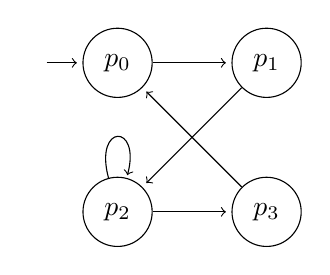
\begin{tikzpicture}[auto, node distance=1cm, shorten >=2pt]
  \node[state,initial,initial text=] (p0) {$p_0$}; 
  \node[state] (p1) [right=of p0] {$p_1$}; 
  \node[state] (p2) [below=of p0] {$p_2$}; 
  \node[state] (p3) [right=of p2] {$p_3$}; 
  \path[->] 
    (p0) edge (p1)
    (p1) edge (p2)
    (p2) edge (p3)
    (p3) edge (p0)
    (p2) edge [loop above] (p2);
\end{tikzpicture}

  \end{center}
  we want to check the following formulas:
  \begin{itemize}
    \item $\displaystyle G \left( \bigwedge^3_{i=0} \Big(p_i \to X \bigvee^3_{\substack{j=0 \\ i \neq j}} p_j \Big) \right)$ is \false, in fact a counterexample is $\tuplev{p_0,p_1,p_2,p_2}$.
    \item $F(p_3)$ is \false and a counterexample is $\tuplev{p_0,p_1} \cdot (p_2)^\w$.
    \item $FG(p_2)$ is also \false and a counterexample is $\big(\tuplev{p_0,p_1,p_2,p_3}\big)^\w$.
  \end{itemize}
\end{example*}

To work on model checking , we'll introduce the following notations:
\begin{itemize}
  \item for each atom $A$, we define $\state{A}$ as the conjunction of all state formulas in $A$ (for first rule in the \nameref{def:p_atom} definition it's satisfiable);
  \item an atom $A$ is \textbf{consistent} with a state $s$ if $s \models \state{A}$, which means that $s$ satisfies all state formulas in $A$;
  \item given a path $\pi = A_0,A_1,\ldots$ in $T_\p$ and a computation $\s = s_0,s_1,\ldots$, we say that $\pi$ is a \textbf{trail} of tableau $T_\p$ over $\s$, if each atom is consistent with the state in the same position, \ie, $A_i$ is consistent with $s_i$;
  \item $\d(A)$ denotes the set of \textbf{successors} of $A$ in the tableau $T_\p$.
\end{itemize}

\begin{definition*}[Behavior graph]
  Given a finite state program $\P$ and a LTL formula $\p$, the behavior graph $\bgraph$ is the product of the graph for $\P$ with the tableau $T_\p$, where:
  \begin{itemize}
    \item nodes are pairs $(s,A)$, with $s$ a state of $\P$ and $A$ an atom consistent with $s$;
    \item initial $\p$-nodes are nodes where $s$ is an initial state and $A$ is an initial $\p$-atom;
    \item $\t$-edges are edges from one node to another ($(s,A) \to (s',A')$) where it holds that the ending state is a \tsuc of the starting one ($s'\,\t\text{-successor}\, s$), and the ending atom is a successor of the starting one ($A' \in \d(A)$).
  \end{itemize}

  \bigskip
  The algorithm that constructs $\bgraph$ works as follows:
  \begin{lstlisting}
    add initial $\p$-nodes to $\bgraph$

    # loops until all nodes/edges are in graph
    for each node $(s,A)$ in $\bgraph$:
      if successor $(s',A')$ not in $\bgraph$:
        add $(s',A')$
        add $\t$-edge from $(s,A)$ to $(s',A')$
  \end{lstlisting}
\end{definition*}

\begin{example}\label{exa:psi-sat}
  The state-transition system LOOP is constructed as follows:
  \begin{itemize}
    \item starts at $x=0$;
    \item the transition relation is $\rho_\t : x' = (x+1) \mod 4$, and $\t_I$ it's just the idling transition;
    \item a weak fair transition $\J = \set{\t}$;
  \end{itemize}

  \begin{center}
    \begin{tikzpicture}[auto, node distance=1cm, shorten >=2pt, state/.style={draw, rounded corners}]

  \node[state] (s0) {$s_0{:}\ \tuplev{x{:}0}$}; 
  \node[above left=0.5cm and 0.5cm of s0] (start) {}; 
  \node[state, below left=of s0] (s1) {$s_1{:}\ \tuplev{x{:}1}$};
  \node[state, below right=of s1] (s2) {$s_2{:}\ \tuplev{x{:}2}$};
  \node[state, below right=of s0] (s3) {$s_3{:}\ \tuplev{x{:}3}$};
  
  \path[->]
    (s0) edge[loop above,distance=0.5cm] node {$\t_I$} (s0)
    (s1) edge[loop left,distance=0.5cm] node {$\t_I$} (s1)
    (s2) edge[loop below,distance=0.5cm] node {$\t_I$} (s2)
    (s3) edge[loop right,distance=0.5cm] node {$\t_I$} (s3);
  
  \path[->]
    (start) edge[bend left] (s0)
    (s0) edge[bend right] node {$\t$} (s1)
    (s1) edge[bend right] node {$\t$} (s2)
    (s2) edge[bend right] node {$\t$} (s3)
    (s3) edge[bend right] node {$\t$} (s0);

\end{tikzpicture}

  \end{center}
  \captionof*{figure}{State-transition graph $G_{\text{LOOP}}$}

  We have a system LOOP and we consider the LTL formula $\psi = \Diamond\msquare(x \neq 3)$.
  In the following tableau figures, the big box means that the states inside share the same prefix.

  \hspace{0.02\textwidth}
  \begin{subfigure}{0.48\textwidth}
    \begin{center}
      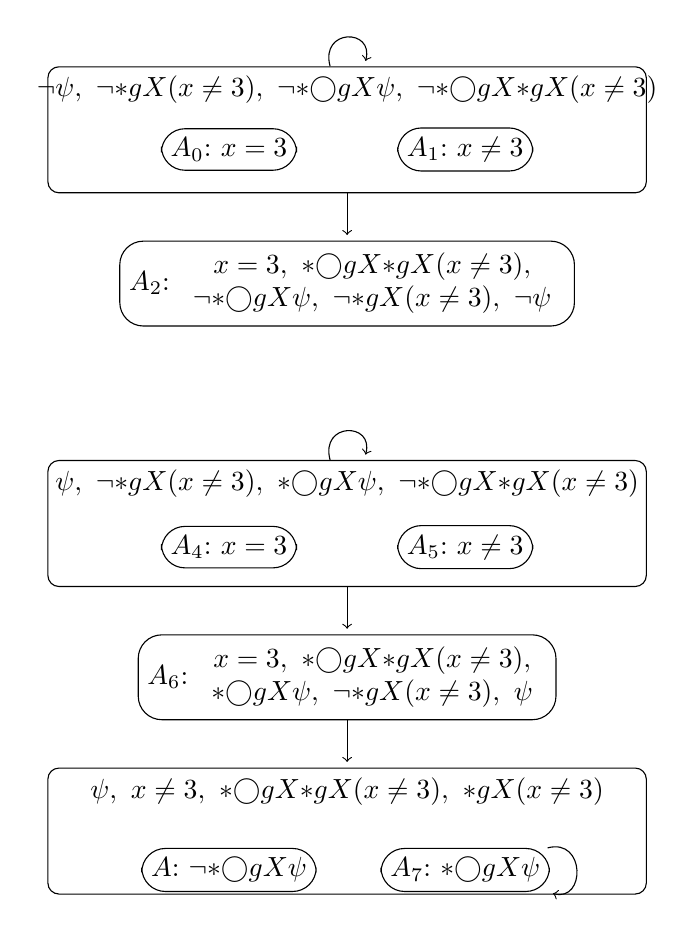
\begin{tikzpicture}[
    state/.style={draw, rectangle, rounded corners=0.3cm},
    box/.style={draw, rectangle, rounded corners, minimum width=7.6cm, minimum height=1.6cm},
    node distance=0.6cm,
    shorten >=2pt
]

  \node[box] (b0) at (0,0) {};
  \node[anchor=north] at (b0.north) {$\neg \psi,\ \neg \msquare(x \neq 3),\ \neg \mcirc \psi,\ \neg \mcirc\msquare(x \neq 3)$};
  \node[state] (a0) at (-1.5,-0.25) {$A_0{:}\ x=3$};
  \node[state] (a1) at (1.5,-0.25) {$A_1{:}\ x\neq 3$};
  \path[->] (b0) edge[loop above,distance=0.5cm] (b0);
  \node[state, below=of b0] (a2) {$A_2{:}\ \begin{array}{c} x=3,\ \mcirc\msquare(x \neq 3),\\ \neg\mcirc \psi,\ \neg\msquare(x \neq 3),\ \neg \psi\end{array}$};
  \path[->] (b0) edge (a2);

  \node[box] (b1) at (0,-5) {};
  \node[anchor=north] at (b1.north) {$\psi,\ \neg \msquare(x \neq 3),\ \mcirc \psi,\ \neg \mcirc\msquare(x \neq 3)$};
  \node[state] (a4) at (-1.5,-5.3) {$A_4{:}\ x=3$};
  \node[state] (a5) at (1.5,-5.3) {$A_5{:}\ x\neq 3$};
  \path[->] (b1) edge[loop above,distance=0.5cm] (b1);
  \node[state, below=of b1] (a6) {$A_6{:}\ \begin{array}{c} x=3,\ \mcirc\msquare(x \neq 3),\\ \mcirc \psi,\ \neg\msquare(x \neq 3),\ \psi\end{array}$};
  \path[->] (b1) edge (a6);
  \node[box, below=of a6] (b2) {};
  \node[anchor=north] at (b2.north) {$\psi,\ x \neq 3,\ \mcirc\msquare (x \neq 3),\ \msquare(x \neq 3)$};
  \node[state] (a3) at (-1.5,-9.4) {$A{:}\ \neg\mcirc \psi$};
  \node[state] (a7) at (1.5,-9.4) {$A_7{:}\ \mcirc \psi$};
  \path[->] (a6) edge (b2);
  \path[->] (a7) edge[loop right,distance=0.5cm] (a7);

\end{tikzpicture}

    \end{center}
    \caption{Complete}
  \end{subfigure}
  \begin{subfigure}{0.48\textwidth}
    \begin{center}
      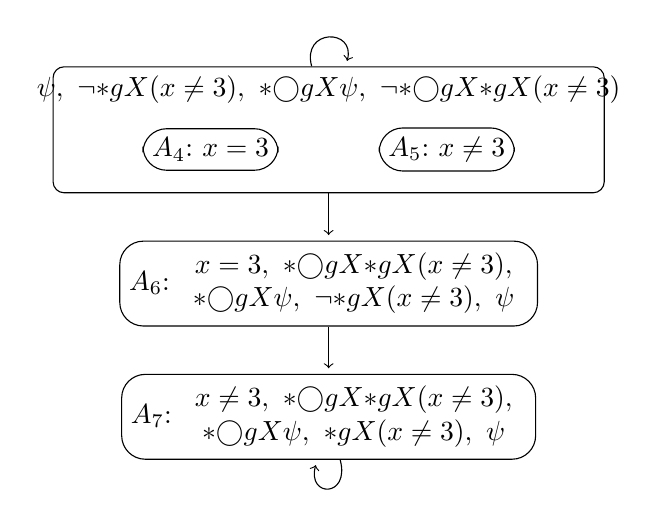
\begin{tikzpicture}[
    state/.style={draw, rectangle, rounded corners=0.3cm},
    box/.style={draw, rectangle, rounded corners, minimum width=7cm, minimum height=1.6cm},
    node distance=0.6cm,
    shorten >=2pt
]

  \node[box] (b1) at (0,0) {};
  \node[anchor=north] at (b1.north) {$\psi,\ \neg \msquare(x \neq 3),\ \mcirc \psi,\ \neg \mcirc\msquare(x \neq 3)$};
  \node[state] (a4) at (-1.5,-0.25) {$A_4{:}\ x=3$};
  \node[state] (a5) at (1.5,-0.25) {$A_5{:}\ x\neq 3$};
  \path[->] (b1) edge[loop above,distance=0.5cm] (b1);

  \node[state, below=of b1] (a6) {$A_6{:}\ \begin{array}{c} x=3,\ \mcirc\msquare(x \neq 3),\\ \mcirc \psi,\ \neg\msquare(x \neq 3),\ \psi\end{array}$};
  \path[->] (b1) edge (a6);

  \node[state, below=of a6] (a7) {$A_7{:}\ \begin{array}{c} x \neq 3,\ \mcirc\msquare(x \neq 3),\\ \mcirc \psi,\ \msquare(x \neq 3),\ \psi\end{array}$};
  \path[->] (a6) edge (a7);
  \path[->] (a7) edge[loop below,distance=0.5cm] (a7);

\end{tikzpicture}

    \end{center}
    \caption{Pruned}
  \end{subfigure}
  \captionof*{figure}{Tableau $T_\psi$}

  \bigskip
  The tableau $T_\psi$ has been pruned in this way because the first connected component of states is not $\p$-reachable, while $A_3$ it's a terminal node, \ie, it doesn't contain a self loop.
  \begin{note}
    Recall that:
    \begin{itemize}
      \item $\mcirc$ is next;
      \item $\Diamond$ is eventually;
      \item $\msquare$ is always.
    \end{itemize}
  \end{note}
  
  \begin{center}
    \begin{tikzpicture}
[
  auto,
  node distance=0.6cm,
  shorten >=2pt,
  state/.style={draw, rectangle, rounded corners=0.3cm, minimum width=1.8cm, minimum height=0.8cm}
]

  \node[state, initial, initial text=] (s0a5) {$(s_0, A_5)$};
  \node[state, below=of s0a5] (s1a5) {$(s_1, A_5)$};
  \node[state, below=of s1a5] (s2a5) {$(s_2, A_5)$};
  \node[state, below left=of s2a5] (s3a4) {$(s_3, A_4)$};
  \node[state, below right=of s2a5] (s3a6) {$(s_3, A_6)$};

  \node[state, initial, initial text=, right=3cm of s0a5] (s0a7) {$(s_0, A_7)$};
  \node[state, below=of s0a7] (s1a7) {$(s_1, A_7)$};
  \node[state, below=of s1a7] (s2a7) {$(s_2, A_7)$};

  \path[->]
    (s0a5) edge[loop right,distance=0.5cm] node {$\t_I$} (s0a5)
    (s1a5) edge[loop right,distance=0.5cm] node {$\t_I$} (s1a5)
    (s2a5) edge[loop right,distance=0.5cm] node {$\t_I$} (s2a5)
    (s3a4) edge[loop left,distance=0.5cm] node {$\t_I$} (s3a4)
    (s0a7) edge[loop right,distance=0.5cm] node {$\t_I$} (s0a7)
    (s1a7) edge[loop right,distance=0.5cm] node {$\t_I$} (s1a7)
    (s2a7) edge[loop right,distance=0.5cm] node {$\t_I$} (s2a7);

  \path[->]
    (s0a5) edge node {$\t$} (s1a5)
    (s1a5) edge node {$\t$} (s2a5)
    (s2a5) edge node {$\t$} (s3a4)
    (s2a5) edge node[swap] {$\t$} (s3a6);

  \path[->]
    (s0a7) edge node {$\t$} (s1a7)
    (s1a7) edge node {$\t$} (s2a7);

  \path[->]
    (s3a4.north) edge[bend left=35] node {$\t$} (s0a5.south west)
    (s3a6.north east) edge[bend left=15] node {$\t$} (s0a7.south west);

  \path[->] (s3a4) edge[bend right=15] node[below] {$\t_I$} (s3a6);

\end{tikzpicture}

  \end{center}
  \captionof*{figure}{Behavior graph $\B_{(\text{LOOP},\psi)}$}

  \bigskip
  Given the LTL formula $\psi$ and an infinite path $\pi$ in $\B_{(\text{LOOP},\psi)}$, $\s_\pi = s_0 s_1 \ldots$ is a run\footnote{Different from a computation, because we don't require fairness (no justice or compassion).}, and $\theta_\pi = A_0 A_1 \ldots$ is a trail of $T_\psi$ over $\s_\pi$.
  However, this is \textit{not sufficient} to prove satisfiability for model checking, because to achieve this, the run $\s_\pi$ should be a \textit{computation} and the trail $\theta_\pi$ should be a \textit{fulfilling trail}.
  For example, the trail $\theta_\pi = (A_5 A_5 A_5 A_4)^\w$ isn't fulfilling, because both $A_4 \andt A_5$ include $\Diamond\msquare(x \neq 3) \andt \neg\msquare(x \neq 3)$.
\end{example}

\begin{definition*}[Adequate subgraph]
  Given a behavior graph $\bgraph$, a subgraph $S \subseteq \bgraph$ has the following properties:
  \begin{itemize}
    \item $\t$ is \textbf{taken} in $S$ if there exists two nodes $(s,A),(s',A') \in S$ \st $(s',A')$ is \tsuc of $(s,A)$;
    \item $S$ is \textbf{just} if every just transition $\t \in \J$ is either taken in $S$ or disabled on some nodes of $S$;
    \item $S$ is \textbf{compassionate} if every compassionate transition $\t \in \C$ is either taken in $S$ or disabled on all nodes of $S$;
    \item $S$ is \textbf{fair} if it's both just and compassionate;
    \item $S$ is \textbf{fulfilling} if every promising formula is fulfilled by an atom $A$ \st, for some state $s$, $(s,A) \in S$;
    \item $S$ is \textbf{adequate} if it's both fair and fulfilling.
  \end{itemize}
\end{definition*}

\begin{example*}[Adequate subgraph]
  We have a system LOOP and we consider the LTL formula $\p \colon \msquare\Diamond(x = 3)$, \ie, $\p = \neg\psi$ where $\psi$ is the LTL formula from previous \autoref{exa:psi-sat}.

  The pruned tableau and the behavior graph $\B_{(\text{LOOP},\p)}$ are the following:
  \begin{center}
    \begin{tikzpicture}[
    state/.style={draw, rectangle, rounded corners=0.3cm},
    box/.style={draw, rectangle, rounded corners, minimum width=7cm, minimum height=1.6cm},
    node distance=0.6cm,
    shorten >=2pt
]

  \node[box] (b1) at (0,0) {};
  \node[anchor=north] at (b1.north) {$\p,\ \Diamond(x = 3),\ \mcirc \p,\ \mcirc\Diamond(x = 3)$};
  \node[state] (a0) at (-1.5,-0.25) {$A_0{:}\ x=3$};
  \node[state] (a1) at (1.5,-0.25) {$A_1{:}\ x\neq 3$};
  \path[->] (b1) edge[loop above,distance=0.5cm] (b1);

\end{tikzpicture}

  \end{center}
  \begin{center}
    \begin{tikzpicture}
[
  auto,
  node distance=0.6cm,
  shorten >=2pt,
  state/.style={draw, rectangle, rounded corners=0.3cm, minimum width=1.8cm, minimum height=0.8cm}
]

  \node[state, initial, initial text=] (s0a1) {$(s_0, A_1)$};
  \node[state, below=of s0a5] (s1a1) {$(s_1, A_1)$};
  \node[state, below=of s1a5] (s2a1) {$(s_2, A_1)$};
  \node[state, below left=of s2a1] (s3a0) {$(s_3, A_0)$};

  \path[->]
    (s0a1) edge[loop right,distance=0.5cm] node {$\t_I$} (s0a1)
    (s1a1) edge[loop right,distance=0.5cm] node {$\t_I$} (s1a1)
    (s2a1) edge[loop right,distance=0.5cm] node {$\t_I$} (s2a1)
    (s3a0) edge[loop left,distance=0.5cm] node {$\t_I$} (s3a0);

  \path[->]
    (s0a1) edge node {$\t$} (s1a1)
    (s1a1) edge node {$\t$} (s2a1)
    (s2a1) edge node {$\t$} (s3a0);

  \path[->]
    (s3a0.north) edge[bend left=35] node {$\t$} (s0a1.south west);

\end{tikzpicture}

  \end{center}

  Is there an adequate SCS?
  This is the case, because the path $\theta_\p = (A_1 A_1 A_1 A_0)^\w$ is fulfilling due to $A_0$ being fulfilling and being taken infinitely often in the path.
  Moreover, is just because the path contains at least one node in which $\t$ is taken (in this case all of them).
  Because it's both fair (due to being just) and fulfilling, by definition of an Adequate subgraph, the subgraph $S = \set{(s_0, A_1),(s_1, A_1),(s_2, A_1),(s_3, A_0)}$ is adequate, therefore it follows that LOOP has a computation that satisfies $\p \colon \msquare\Diamond(x = 3)$ and the formula is $\p$-valid.
\end{example*}

Justice holds for supergraphs\footnote{bigger graphs, opposite of subgraph}, which implies that if a graph it's not just, then all its subgraphs will be also not just.
Because justice holds for supergraphs, we first may think that to find and adequate subgraph we can just check MSCS.
However, compassion doesn't hold for supergraphs, because we could have a supergraph not compassionate while the inner graph is, thus is completely possible that the graph is adequate, while the supergraph isn't.
That's why MSCS checking is not enough to find adequate subgraphs.

\begin{example*}[Counterexample for MSCS checking not enough]
  In this example is shown that a compassionate graph $S'$ doesn't imply that a supergraph $S$ is compassionate ($S' \subseteq S$).
  The graph $S$ is the following: 
  \begin{center}
    \begin{tikzpicture}[auto, node distance=1cm, shorten >=2pt, state/.style={draw, rounded corners}]

  \node (s0) {$\dots$}; 
  \node[state, right=of s0] (s1) {$s_1, A_3$};
  \node[state, right=of s1] (s2) {$s_2, A_4$};
  \node[right=of s2] (s3) {};

  \path[->]
    (s0) edge (s1)
    (s1) edge[bend left] node {$\t_1$} (s2)
    (s2) edge[bend left] node {$\t_1$} (s1)
    (s2) edge node {$\t_2$} (s3);

\end{tikzpicture}

  \end{center}
  where $\t_2$ is a compassionate transition, which is enabled on $s_2$ and disabled on $s_1$.
  Intuitively, considering $S'$ as the SCC\footnotemark composed of only $s_1$, we have that $\t_2$ is not enabled.
  Thus, if we remain in $s_1$ forever, we have that compassion holds because $t_2$ is never enabled and no rule is violated.
  On the other hand, considering the entire graph $S$, we have that compassion is violated because is enabled in $s_2$ and never taken.
  This is a clear example of a supergraph $S$ which is not adequate, while the graph $S'$ is.
\end{example*}
\footnotetext{Strongly Connected Component}

The algorithm for finding an adequate subgraph is the following:
\begin{lstlisting}
  # input: SCS $S$
  # output: SCS $S'$ ($\subseteq S$)
  adequateSub($S$):
    if $S$ not fulfilling or $S$ not just:
      return $\emptyset$
    if $S$ compassionate:
      return $S$

    # If we're here is means that $S$ is fulfilling and just
    # but not compassionate.

    $T$ = set of compassionate trasitions not taken
    # We denote with EN($\t$,$S$) the set of all nodes ($s$,$A$) in $S$
    # on which $\t$ is enabled.
    # Because of $T$ definition, we have that $\text{EN}(T,S) \neq \emptyset$.

    $U$ = $S$ - EN($T$,$S$)
    Decompose $U$ into MSCSs $U_1$, $\dots$, $U_k$. 
    $V$ = $\emptyset$

    for $U_i$ in $U$:
      if $V \neq \emptyset$:
        break
      else:
        $V$ = adequateSub($U_i$) # recursion
    return $V$
\end{lstlisting}

\begin{note}
  Note that if the algorithm output is $\emptyset$ it means that $S$ contains no adequate subgraph.
\end{note}

\begin{example*}
  The state-transition system LOOP+ is constructed as follows:
  \begin{itemize}
    \item starts at $x=0$;
    \item $\t_I$ it's just the idling transition;
    \item justice is required for $\J = \set{\t_1,\t_2}$;
    \item compassion is required for $\C = \set{\t_3}$.
  \end{itemize}

  \begin{center}
    \begin{tikzpicture}[auto, node distance=1cm, shorten >=2pt, state/.style={draw, rounded corners}]

  \node[state] (s0) {$s_0{:}\ \tuplev{x{:}0}$}; 
  \node[below left=-0.2cm and -0.4cm of s0] (s0l) {}; 
  \node[below right=-0.2cm and -0.4cm of s0] (s0r) {}; 
  \node[above left=0.5cm and 0.5cm of s0] (start) {}; 
  \node[state, below left=of s0] (s1) {$s_1{:}\ \tuplev{x \colon 1}$};
  \node[state, below right=of s1] (s2) {$s_2{:}\ \tuplev{x{:}2}$};
  \node[above left=-0.2cm and -0.4cm of s2] (s2l) {}; 
  \node[above right=-0.2cm and -0.4cm of s2] (s2r) {}; 
  \node[state, below right=of s0] (s3) {$s_3{:}\ \tuplev{x{:}3}$};
  
  \path[->]
    (start) edge[bend left] (s0)
    (s0) edge[loop above,distance=0.5cm] node {$\t_I$} (s0)
    (s1) edge[loop left,distance=0.5cm] node {$\t_I$} (s1)
    (s2) edge[loop below,distance=0.5cm] node {$\t_I$} (s2)
    (s3) edge[loop right,distance=0.5cm] node {$\t_I$} (s3);
  
  \path[->, red]
    (s0) edge[bend right] node {$\t_1$} (s1)
    (s1) edge[bend right] node {$\t_1$} (s2)
    (s2r) edge node[anchor=north west] {$\t_1$} (s0r);

  \path[->, green]
    (s2) edge[bend right] node {$\t_2$} (s3)
    (s3) edge[bend right] node {$\t_2$} (s0)
    (s0l) edge node[anchor=south east] {$\t_2$} (s2l);

  \path[->, brown]
    (s1) edge node {$\t_3$} (s3);

\end{tikzpicture}

  \end{center}
  \captionof*{figure}{State-transition graph $G_{\text{LOOP+}}$}
  The LTL formula that we consider is $\psi \colon \Diamond\msquare(x \neq 3)$.

  \begin{center}
    \input{tikz/ex4_tableau_pruned.tikz}
  \end{center}
  \captionof*{figure}{Pruned tableau $T_\psi$}

  \begin{center}
    \begin{tikzpicture}
[
  auto,
  node distance=0.6cm,
  shorten >=2pt,
  state/.style={draw, rectangle, rounded corners=0.3cm, minimum width=1.8cm, minimum height=0.8cm}
]

  \node[state, initial, initial text=] (s0a5) {$(s_0, A_5)$};
  \node[state, below=of s0a5] (s1a5) {$(s_1, A_5)$};
  \node[right=-0.15cm of s1a5] (s1a5l) {$\t_I$};
  \node[state, below=of s1a5] (s2a5) {$(s_2, A_5)$};
  \node[state, below left=of s2a5] (s3a4) {$(s_3, A_4)$};
  \node[state, below right=of s2a5] (s3a6) {$(s_3, A_6)$};

  \node[state, initial, initial text=, right=3cm of s0a5] (s0a7) {$(s_0, A_7)$};
  \node[state, below=of s0a7] (s1a7) {$(s_1, A_7)$};
  \node[right=-0.15cm of s1a7] (s1a7l) {$\t_I$};
  \node[state, below=of s1a7] (s2a7) {$(s_2, A_7)$};

  \path[->]
    (s0a5) edge[loop right,distance=0.5cm] node {$\t_I$} (s0a5)
    (s1a5) edge[loop right,distance=0.5cm] (s1a5)
    (s2a5) edge[loop right,distance=0.5cm] node {$\t_I$} (s2a5)
    (s3a4) edge[loop left,distance=0.5cm] node {$\t_I$} (s3a4)
    (s0a7) edge[loop right,distance=0.5cm] node {$\t_I$} (s0a7)
    (s1a7) edge[loop right,distance=0.5cm] (s1a7)
    (s2a7) edge[loop below,distance=0.5cm] node {$\t_I$} (s2a7)
    (s3a4) edge[bend right=15] node[below] {$\t_I$} (s3a6);

  \path[->, red]
    (s0a5) edge node {$\t_1$} (s1a5)
    (s1a5) edge node {$\t_1$} (s2a5)
    (s0a7) edge node {$\t_1$} (s1a7)
    (s1a7) edge node {$\t_1$} (s2a7)
    (s2a5.north east) edge[bend right=55] node[swap] {$\t_1$} (s0a5.south east)
    (s2a7.north east) edge[bend right=55] node[swap] {$\t_1$} (s0a7.south east);

  \path[->, green]
    (s2a5) edge node {$\t_2$} (s3a4)
    (s2a5) edge node[swap] {$\t_2$} (s3a6)
    (s3a4.north) edge[bend left=35] node {$\t_2$} (s0a5.west)
    (s3a6.north east) edge[bend left=35] node {$\t_2$} (s0a7.west)
    (s0a5.south west) edge[bend right=25] node[swap] {$\t_2$} (s2a5.north west)
    (s0a7.south west) edge[bend right=25] node[swap] {$\t_2$} (s2a7.north west);

  \path[->, brown]
    (s1a5.south west) edge[bend right=25] node {$\t_3$} (s3a4.north)
    (s1a5.south east) edge[bend left=25] node {$\t_3$} (s3a6.north);


\end{tikzpicture}

  \end{center}
  \captionof*{figure}{Behavior graph $\B_{(\text{LOOP+},\psi)}$}

  \bigskip
  \textit{Do we expect that the formula $\psi$ is P-sat or not?}

  At the beginning, because we start with x=0 (which is $\neq 3$) the formula is satisfied.
  The cycle ($s_0,s_1,s_2$) has the problem that we have justice for $\t_1$ but we miss compassion for $\t_3$ which is required, but from the system loop we can see that is enabled infinitely often but taken finitely often, in particular 0 times, because in this cycle we don't reach $s_3$.
  For ($s_0,s_2,s_3$) instead we have that we fulfill both justice ($\t_2$ taken) and compassion (because we don't take $\t_3$ thus compassion not required), but the formula isn't good because there is no point at which the cycle stabilizes to a value $\neq 3$.
  However, the cycle ($s_0,s_2$) respects justice and compassion, plus has values always different from 3, thus fulfills both the formula and the fairness constraints.

  In fact from the behavior graph we can consider the SCS on the right, which has the problem of having $s_1$ in the middle for which is required compassion.
  If we remove the middle node $(s_1, A_7)$ and its respective edges from this subgraph we end with the following \textbf{adequate subgraph}:
  \begin{center}
    \begin{tikzpicture}
[
  auto,
  node distance=0.6cm,
  shorten >=2pt,
  state/.style={draw, rectangle, rounded corners=0.3cm, minimum width=1.8cm, minimum height=0.8cm}
]

  \node[state, initial, initial text=] (s0a7) {$(s_0, A_7)$};
  \node[state, below=of s0a7] (s2a7) {$(s_2, A_7)$};

  \path[->]
    (s0a7) edge[loop above,distance=0.5cm] node {$\t_I$} (s0a7)
    (s2a7) edge[loop below,distance=0.5cm] node {$\t_I$} (s2a7);

  \path[->, red]
    (s2a7.north east) edge[bend right=25] node[swap] {$\t_1$} (s0a7.south east);

  \path[->, green]
    (s0a7.south west) edge[bend right=25] node[swap] {$\t_2$} (s2a7.north west);

\end{tikzpicture}

  \end{center}
\end{example*}

We refer to \textbf{SAT} to mean that we check whether a temporal formula $\p$ is satisfiable, while with \textbf{P-SAT} we refer to satisfiability of a formula $\p$ over a program P.

\begin{definition*}[P-SAT algorithm]
  \begin{itemize}
    \item First construct the state transition graph $G_P$, the pruned tableau $T_\p$ and the behavior graph $\B_{(P,\p)}$;
    \item Then decompose $\B_{(P,\p)}$ into MSCs $S_1,\dots,S_t$;
    \item Last apply \texttt{adequateSub} algorithm on each MSC $S_i$: if any of these returns a non-empty result, then there exists a computation of P satisfying $\p$.
  \end{itemize}
\end{definition*}
From this definition we can derive that if there is a P-computation that satisfies $\neg\p$ then $\p$ can't be P-valid.
On the other hand it also means that if it doesn't exist a computation for P that satisfies $\neg\p$, this implies that $\p$ is P-valid.

\section{CTL Model Checking}

Recall the CTL syntax and semantics from the previous chapter; here we turn them into an algorithm. The shorthand equivalences given there -- $\EF$, $\AF$, $\EG$, $\AG$ expressed through $\EU$ and $\AU$ -- are exactly what drive the recursion. Cases like $\EX \andt \AX$ are resolved by visiting the successors, while $\EU \andt \AU$, in the worst case, require visiting all the nodes reachable by a path from the current state.
For this reason we can express the until $\UU$ as:
\begin{itemize}
  \item $\EU(\a,\b) = \b \lor \big(\a \land \EX \EU(\a,\b)\big)$
  \item $\AU(\a,\b) = \b \lor \big(\a \land \AX \AU(\a,\b)\big)$
\end{itemize}
which imposes that either is now and all in the following, or, if it's not satisfied now, we postpone the constraint to the successor.

\begin{lstlisting}[title={CTL Model Checking algorithm}]

  def ctlModelChecker(M=$\langle$S,R,L$\rangle$):
    for i in range(|$\a$|):
      for $\b$ in Sub($\a$):
        if |$\b$| == i:
          match $\b$:

            case P:   # propositional case
              for s in S:
                  # if all propositional letters in P belong
                  # to the labeling of node s, then are all
                  # added to its labeling.
                  if $\forall$ p $\in$ P; p $\in$ L(s):
                    L(s).append($P$)

            case EX$\y$:
              for s in S:
                if $\exists$ t; Rst and $\y \in $ L(t):
                  L(s).append($\b$)

            case AX$\y$:
              for s in S:
                if $\forall$ t; Rst $\implies$ $\y \in $ L(t):
                  L(s).append($\b$)

            case EU($\y$,$\d$):
              for s in S:
                marked(s) = False
              for s in S:
                if $\d \in$ L(s):
                  checkEU(M,s,$\y$,$\d$)

            case AU($\y$,$\d$):
              for s in S:
                marked(s) = $\false$
              for s in S:
                if not marked(s):
                  checkAU(M,s,$\y$,$\d$)


  def checkEU(M,s,$\y$,$\d$):
    if not marked(s):
      marked(s) = True
      L(s).append(EU($\y$,$\d$)

      for t in S:
        if Rts and $\y \in$ L(t):
          checkEU(M,t,$\y$,$\d$)


  def checkAU(M,s,$\y$,$\d$):
    if marked(s):
      if AU($\y$,$\d$) $\in$ L(s):
        return True
      else:
        return False

    marked(s) = True
    if $\d \in$ L(s):
      L(s).append(AU($\y$,$\d$)
      return True

    if $\y \notin$ L(s):
      return False

    for t in S:
      if Rst and not checkAU(M,t,$\y$,$\d$):
        return False

    L(s).append(AU($\y$,$\d$)
    return True
\end{lstlisting}

The CTL model checker has complexity $O\big(\abs{\a} \cdot (\abs{S} + \abs{R})\big)$, \ie, it is \emph{polynomial} -- in fact linear -- in both the formula size and the model size, which makes CTL model checking one of the most tractable verification problems. The practical bottleneck is therefore \emph{not} the algorithm but the \textbf{state-space explosion}: realistic systems have $\abs{S}$ in the billions, so even a linear scan is infeasible unless the state set is represented \emph{symbolically} -- which is exactly what the next sections do.

\section{Symbolic Model Checking}

Classical algorithms for model checking belongs to the class of \emph{explicit-state} model checking, in which state are explicitly represented and considered individually.
However, model checking is affected by the \textbf{state-space explosion} problem, which consists of: suppose that the system $M$ is composed of several subcomponents, \eg, $M = M_1 \times \dots \times M_n$, this implies that the number of states is exponential in $n$ and thus it could be that the state space is so huge that cannot be explored by a linear time algorithm.
Usually the state size that is computable by an explicit model checker is $\approx 10^6$ states.
That's the reason why Symbolic model checking is born.

In Symbolic model checking is constructed such that we don't reason upon single states, rather with set of states.
Moreover, we will work no more with Kripke structures but with Boolean formulas instead.
The Boolean encoding of a Kripke structure $M = (S,I,T,L)$ is:
\begin{itemize}
  \item $\ol{x} = \set{x_0, \dots, x_{n-1}}$ is a set of Boolean states;
  \item $S = \set{0,1}^n$ is a \quoted{state} and represents an assignment to all the state variables, \ie, is like a big vector of binary values\footnote{With $n$ values we can represent $2^n$ states};
  \item the symbolic initial state is an assignment $\ol{x}$ that satisfies a Boolean formula $f_I$ which encodes the initial states $I$ of the Kripke structure $M$;
  \item the symbolic transition relation is the same of the initial states, just with two assignments $\ol{x}'$ and the Boolean formula is called $f_T$;
  \item for each label $p \in \text{range}(L)$ is introduced a Boolean formula $f_p$ that represents all the states that are labeled with $p$.
\end{itemize}
A Symbolic Transition System (STS) is represented by a tuple $\tuple{\ol{x}, f_I, f_T, \set{f_{p_1}, \dots, f_{p_k}}}$, but for simplicity of notation we'll keep $(S,I,T,L)$. 

A path is just an infinite sequence of assignments to the state variables, \st the initial assignment belongs to the initial state assignments and for each couple of consequent assignments exists a transition relation.

Computing the predecessors (or successors) of a symbolically-represented set of states amounts to composing such Boolean formulas and then \emph{eliminating} the intermediate variables by quantification. We use Quantified Boolean formulas to connect Boolean formulas: $\p (\overrightarrow{w},\overrightarrow{x}) = \exists \overrightarrow{v} \big( f(\overrightarrow{v},\overrightarrow{w}) \land g(\overrightarrow{v},\overrightarrow{x}) \big)$.
We have that:
\begin{itemize}
  \item $\exists x \underbrace{f}_{\text{OBDD}} \equiv f \vert_{x \leftarrow 0} \underbrace{\lor}_{\text{Apply}} f \vert_{x \leftarrow 1}$
  \item $\forall x f \equiv f \vert_{x \leftarrow 0} \land f \vert_{x \leftarrow 1}$
\end{itemize}
For this to pay off we need a representation of Boolean functions that is \emph{compact}, \emph{canonical} (so equivalence is cheap), and that supports these two primitives efficiently: Boolean combination ($\lor / \land$, the \emph{Apply} operation) and variable fixing (the \emph{Restrict} operation used above for quantification). Ordered Binary Decision Diagrams are that representation, and the whole CTL fixpoint computation reduces to operations on them.

\section{Ordered Binary Decision Diagrams}

Ordered Binary Decision Diagrams (OBDD) are a reduced version of decision trees for Boolean functions, therefore here's a quick summary on Binary Decision Trees (BDT):
\begin{itemize}
  \item nodes are split into terminal/leaf and non-terminal/internal;
  \item each non-terminal nodes $v$ is labelled by a variable $\var(v)$ and has exactly 2 successors $\low(v)$ and $\high(v)$, which are respectively its left and right children;
  \item internal nodes at the same height\footnote{Distance from root.} have the same label;
  \item each leaf $v$ is labelled with $\val(v) \in \set{0,1}$.
\end{itemize}
The issue with BDT is that it's very redundant, generating too many isomorphic subtrees and leaves.

Every OBDD with root $v$ defines a Boolean function $f_v(x_1, \dots, x_n)$ as follows:
\begin{itemize}
  \item if $v$ is a leaf, then $f_v(x_1,\dots,x_n) = \val(v)$;
  \item if $v$ is an internal node and $\text{var}(v) = x_i$, then
    \begin{equation*}
      f_v(x_1,\dots,x_n) = \left( \neg x_i \land f_{\low(v)}(x_1,\dots,x_n) \right) \lor \left( x_i \land f_{\high(v)}(x_1,\dots,x_n) \right)
    \end{equation*}
    \ie, goes recursively in the value of the right/left child respectively if the variable $x_i$ is \true or not.
\end{itemize}

The following figure represents the comparison of a BDT against an OBDD for the formula $x_1 \land (x_2 \lor x_3)$:
\begin{figure}[H]
  \centering
  \begin{subfigure}{0.48\textwidth}
    \begin{center}
      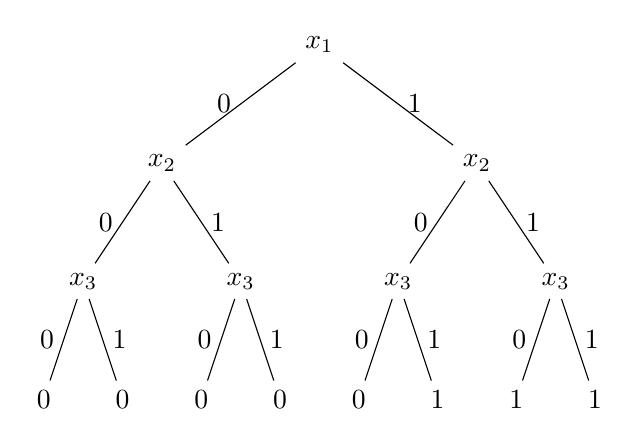
\begin{tikzpicture}
  [level 1/.style={sibling distance=4cm},
  level 2/.style={sibling distance=2cm},
  level 3/.style={sibling distance=1cm}]
  \node at (0,0) {$x_1$}
      child {
          node {$x_2$}
          child {
            node {$x_3$}
            child {
              node {0}
              edge from parent node[left] {0}
            }
            child {
              node {0}
              edge from parent node[right] {1}
            }
            edge from parent node[left] {0}
          }
          child {
            node {$x_3$}
            child {
              node {0}
              edge from parent node[left] {0}
            }
            child {
              node {0}
              edge from parent node[right] {1}
            }
            edge from parent node[right] {1}
          }
          edge from parent node[left] {0}
      }
      child {
          node {$x_2$}
          child {
            node {$x_3$}
            child {
              node {0}
              edge from parent node[left] {0}
            }
            child {
              node {1}
              edge from parent node[right] {1}
            }
            edge from parent node[left] {0}
          }
          child {
            node {$x_3$}
            child {
              node {1}
              edge from parent node[left] {0}
            }
            child {
              node {1}
              edge from parent node[right] {1}
            }
            edge from parent node[right] {1}
          }
          edge from parent node[right] {1}
      };
\end{tikzpicture}

    \end{center}
  \end{subfigure}
  \begin{subfigure}{0.48\textwidth}
    \begin{center}
      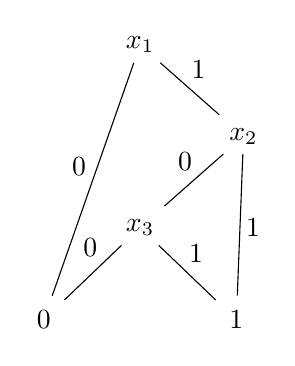
\begin{tikzpicture}[auto, node distance=1cm, shorten >=2pt]
  \node (x1) {$x_1$}; 
  \node (x2) [below right=of x1] {$x_2$}; 
  \node (x3) [below left=of x2] {$x_3$}; 
  \node (out0) [below left=of x3] {0}; 
  \node (out1) [below right=of x3] {1}; 
  \path[-]
    (x1) edge node[pos=0.4,inner sep=2pt] {1} (x2)
    (x1) edge node[inner sep=2pt,swap] {0} (out0)
    (x2) edge node[pos=0.4,inner sep=2pt,swap] {0} (x3)
    (x2) edge node[inner sep=2pt] {1} (out1)
    (x3) edge node[pos=0.3,inner sep=2pt,swap] {0} (out0)
    (x3) edge node[pos=0.4,inner sep=2pt] {1} (out1);
\end{tikzpicture}

    \end{center}
  \end{subfigure}
  \caption*{Comparison of Decision tree against OBDD}
\end{figure}

Besides being compact, OBDD provides a \textbf{canonical form} of the Boolean formula, \ie, once the order of the tree variables is fixed, then it exists only one unique (minimal) OBDD for that formula.
This is different from BDT where order doesn't matter because it doesn't change the size of the tree.
Moreover, the canonical form property is crucial because allows solving equivalence of formula in a very efficient way, because the formula equivalency problem can be reduced to a tree isomorphism problem, \ie, checking if the trees are the same.

The algorithm for reducing redundancy is:
\begin{enumerate}
  \item \textbf{remove duplicated leaves}: leave only one leaf for each value, while all the other copies must be deleted, and edges rerouted;
  \item \textbf{remove duplicated internal nodes}: the same process done for the leaves is applied to node variables: given two different nodes $u,v$, if it holds that:
    \begin{itemize}
      \item $\var(u) = \var(v)$;
      \item $\low(u) = \low(v)$, \ie, their left child must be the same node (different from saying that it must have the same value);
      \item $\high(u) = \high(v)$, same concept for left, but for right child;
    \end{itemize}
    then one between $u$ and $v$ must be deleted and its incoming edges reconnected to the other;
  \item \textbf{remove redundant trees}: if an internal node $v$ has $\low(v) = \high(v)$, \ie, its left and right children are equal, then eliminate the node $v$ and connect directly its incoming edge to one of his children (it doesn't matter which because they're equal).
\end{enumerate}
These rules are applied in order (from 1 to 3), but after having applied rule 3, it can happen that we can re-apply rule 2, and then apply again rule 3, and we proceed in this way until it stabilizes.
However, what's important to notice is that after having fixed the variable order, the order in which we apply the rules is irrelevant because we will end with the same unique minimal OBDD.

Even though the problem of finding an optimal ordering is NP-complete, by working with heuristics, like keeping variables that are close in the formula as close as possible in the OBDD as well, we can compute an OBDD tree that is still very efficient.

\subsection{Encoding of Boolean operators}

To encode Boolean operators we introduce a function called \textbf{restrict}, which allows to restrict some argument $x_i$ of the Boolean function $f$ to assume a constant value $b \in \set{0,1}$, \ie, the function becomes $f(x_1,\dots,x_{i-1},b,x_{i+1},\dots,x_n)$;
The application of this function has an effect equal to removing the outgoing edges of $x_i$ labelled with $\neg b$.

\subsection{Encoding of temporal operators}

To encode operators of a temporal logic like CTL we can use predicate transformers, but before explain it we need to introduce the concept of \textbf{fixpoint}.
\begin{definition*}[Fixpoint]
  Given a function $\t: \text{Powerset}(S) \to \text{Powerset}(S)$ and taken any $S' \subseteq S$, it's a fixpoint if
  \begin{equation*}
    \t(S') = S'
  \end{equation*}
\end{definition*}
The set of states that satisfy a given CTL formula will be characterized as the least/greatest fixpoint of a suitable function.

Let $M = (S,R,L)$ a finite Kripke structure, the Powerset$(S)$ can be viewed as a lattice under the set ordered respect to inclusion, where the bottom (least element) of the lattice is $\emptyset$ and its top (greatest element) is equal to $S$, while in the middle we will have all the possible subsets.

$\t$ is a predicate transformer and has the following properties:
\begin{itemize}
  \item is \textbf{monotonic} if given two sets $P,Q$, with $P \subseteq Q$, it holds that $\t(P) \subseteq \t(Q)$;
  \item is \textbf{$\bigcup$-continuous} if given $P_1 \subseteq P_2 \subseteq \dots$ it holds that $\t\left(\bigcup_i P_i\right) = \bigcup_i \t(P_i)$;
  \item is \textbf{$\bigcap$-continuous} if given $P_1 \supseteq P_2 \supseteq \dots$ it holds that $\t\left(\bigcap_i P_i\right) = \bigcap_i \t(P_i)$.
\end{itemize}
Moreover, we write $\t^i(Z)$ to denote $i$ consecutive application of predicate $\t$ to the set $Z$.

\begin{definition*}[Tarski]
  A monotonic predicate transformer $\t$ on Powerset$(S)$ has a least fixpoint, denoted with $\mu z . \t z$, and a greatest fixpoint, denoted with $\nu Z . \t Z$, where
  \begin{itemize}
    \item $\mu Z . \t Z = \bigcap \set{Z \colon \t(Z) \subseteq Z}$
    \item $\nu Z . \t Z = \bigcup \set{Z \colon \t(Z) \supseteq Z}$
  \end{itemize}

  Moreover, if $\t$ is not only monotonic but is also
  \begin{itemize}
    \item $\bigcup$-continuous, then it holds that $\mu Z . \t Z = \bigcup_i \t^i(\false)$, \ie, we can reach the fixpoint going upwards, starting from the empty-set at the bottom, in a finite number of steps (it cannot increase forever), which is a typical construction for existential modalities;
    \item $\bigcap$-continuous, then it holds that $\nu Z . \t Z = \bigcap_i \t^i(\true)$, \ie, we can reach the fixpoint starting from $S$ and going downwards in a finite number of steps (it cannot decrease forever), which is a typical construction for universal modalities.
  \end{itemize}
\end{definition*}

\begin{lemma*}
  If $S$ is finite and $\t$ is monotonic, then $\t$ is also continuous with respect to $\bigcup \andt \bigcap$.
\end{lemma*}

Because in the previous definition $S$ was always finite, due to this lemma, we have that the two continuous rules can always be applied.

\begin{lemma*}
  If $\t$ is monotonic, then for every $i$:
  \begin{itemize}
    \item $\t^i (\false) \subseteq \t^{i+1} (\false)$
    \item $\t^{i+1} (\true) \subseteq \t^i (\true)$
  \end{itemize}
\end{lemma*}

\begin{lstlisting}[title={Least/Greatest Fixpoints}]

def leastFixpoint():
  $Q$ = false
  $Q'$ = $\t$(false)
  while $Q$ != $Q'$:
    $Q$ = $Q'$
    $Q'$ = $\t$($Q'$)
  return $Q$


def greatFixpoint():
  $Q$ = true
  $Q'$ = $\t$(true)
  while $Q$ != $Q'$:
    $Q$ = $Q'$
    $Q'$ = $\t$($Q'$)
  return $Q$
\end{lstlisting}

Let us introduce the predicate transformer association for CTL operators:
\begin{itemize}
  \item $\AF f_1 = \mu Z. f_1 \lor \AX Z$
  \item $\EF f_1 = \mu Z. f_1 \lor \EX Z$
  \item $\AG f_1 = \nu Z. f_1 \land \AX Z$
  \item $\EG f_1 = \nu Z. f_1 \land \EX Z$
  \item $\AA[f_1 \UU f_2] = \mu Z. f_2 \lor (f_1 \land \AX Z)$
  \item $\EE[f_1 \UU f_2] = \mu Z. f_2 \lor (f_1 \land \EX Z)$
\end{itemize}
The negation of the until operator $\UU$ is the release operator $\RRR$, which follows the same two rules for the until, except that it's based on the greatest fixpoint $\nu$, instead of the least fixpoint $\mu$.

For operators $\AX \andt \EX$ we don't need any fixpoint because we just need to check the successor.

%\begin{definition*}[]
%  
%\end{definition*}

\section{Planning as Symbolic Model Checking}

Planning problems can be naturally encoded as symbolic model checking problems over a Kripke structure, allowing us to exploit the OBDD-based machinery developed in the previous sections.

A \textbf{planning problem} is a triple $\langle \mathcal{S}, \mathcal{A}, \mathcal{G} \rangle$ where:
\begin{itemize}
  \item $\mathcal{S}$ is a set of states, described by a set of propositional variables $\overrightarrow{x} = (x_1, \dots, x_n)$, so that $|\mathcal{S}| \le 2^n$;
  \item $\mathcal{A}$ is a set of actions, each with a precondition and an effect, encoded as a transition relation $R(\overrightarrow{x}, \overrightarrow{x'})$;
  \item $\mathcal{G} \subseteq \mathcal{S}$ is a set of goal states, described by a propositional formula $\mathit{goal}(\overrightarrow{x})$.
\end{itemize}
The planning task is to find a sequence of actions that leads from an initial state $s_0 \models I(\overrightarrow{x})$ to a state satisfying the goal.

\paragraph{Encoding as model checking.}
We define a symbolic Kripke structure $M = (\overrightarrow{x}, I, R, \mathit{goal})$ exactly as in the symbolic model checking framework.
Solving the planning problem then reduces to checking whether $\mathit{goal}(\overrightarrow{x})$ is reachable from the initial states, \ie, whether
\begin{equation*}
  M \models E\,\mathit{true}\,\mathcal{U}\,\mathit{goal}
\end{equation*}
which, in terms of the fixpoint characterisation of CTL, is equivalent to computing
\begin{equation*}
  \mu Z.\; \mathit{goal} \lor \EX Z
\end{equation*}
starting from $Z = \bot$ and iterating until a fixpoint is reached.
Each iteration expands the reachable set by one step backwards through the transition relation:
\begin{equation*}
  \llbracket \EX Z \rrbracket = \exists \overrightarrow{x'} \bigl( R(\overrightarrow{x}, \overrightarrow{x'}) \land Z(\overrightarrow{x'}) \bigr)
\end{equation*}
All intermediate sets are represented as OBDDs, and existential quantification over $\overrightarrow{x'}$ is computed via the \textit{Restrict} and \textit{Apply} operations already introduced.

\paragraph{Plan extraction.}
Once the fixpoint has been computed and $s_0$ is found to lie in the reachable set, a concrete plan can be extracted by tracing forward: at each step, pick any action whose precondition is satisfied and whose effect moves the current state closer to the goal (according to the precomputed layers of the fixpoint). The plan length is bounded by the number of fixpoint iterations required to reach the goal, which in turn is bounded by $|\mathcal{S}|$.

\paragraph{Complexity and practical considerations.}
The symbolic approach avoids explicit state enumeration and can handle systems with $2^n$ states using OBDDs of size polynomial in $n$ (in favourable variable orderings). In the worst case, however, OBDDs can be exponential; finding an optimal variable order is NP-complete, so heuristics are used in practice. Classical planning solvers such as \texttt{BDD-based planners} directly exploit this encoding.

\section{Bounded Model Checking}

SAT-based Symbolic model checking is also known as Bounded Model Checking (BMC).
Because model checking of a formula $\p$ is a universal problem, which means that we have to compute all the possibilities for $\p$, we can change how we reason about it and tackle the problem from the perspective of an emptiness problem, \ie, if there exist a computation that satisfies $\neg \p$.
In this way we're able to transform a universal problem into an existential one, which of course the two problem equals in the case that the model $M$ models the formula $\p$, because it means that it doesn't exist a computation that satisfies $\neg \p$.

Bounded Model Checking works on the emptiness incrementally, \ie, checks if exists an execution $\pi$ of $M$ of length $k$ that satisfies $\p$, by encoding the problem into a SAT instance and solves it with a SAT solver.
If the solver found something it means that a counterexample for $\p$ has been found, otherwise the length $k$ is incremented and the previous step is repeated.

An infinite state sequence can still be represented as a finite trace if it contains a loop back.

\begin{definition*}[$k$-loop (or lasso-shaped)]
  A path $\pi$ is a $(k,l)$-loop, with $l \leq k$, if $T(\pi(k),\pi(l))$ holds, \ie, there is a transition from $k$ to $l$ and the path can be expressed as $\pi = u v^\w$, where:
  \begin{itemize}
    \item $u = \pi(1)\dots\pi(l-1)$;
    \item $v = \pi(l)\dots\pi(k)$.
  \end{itemize}
  We call $\pi$ a $k$-loop if there exists $l \leq k$ for which $\pi$ is a $(k,l)$-loop.
  \begin{center}
    \begin{tikzpicture}[shorten >=4pt]
  \foreach \x in {0,1,2,3,4,5} {
    \draw[fill] (\x,0) circle (.2ex);
  }
  \foreach \x in {0,1,2,4} {
    \draw[->] (\x,0) -- (\x+1,0);
  }
  \draw[dashed,->] (3,0) -- (4,0);
  \path[->] (5,0) edge[bend right=50] (2,0);
  \node[below] at (2,0) {$l$};
  \node[below] at (5,0) {$k$};
\end{tikzpicture}

  \end{center}
\end{definition*}

Given a finite trace $\pi$, BMC distinguishes these two cases:
\begin{itemize}
  \item $\pi$ contains a $k$-loop, then BMC applies standard LTL semantics to check if $\pi \models \p$;
  \item $\pi$ is loop-free, then BMC applies bounded semantics.
\end{itemize}
Note that if a path is a model of $\p$ under bounded semantics, then this path is also a model of $\p$ under standard semantics.

\begin{definition*}[Bounded semantics for LTL]
  Given $k \geq 0 \andt \pi$ a path that doesn't contain a $k$-loop, like so
  \begin{center}
    \input{tikz/loop-free.tikz}
  \end{center}
  an LTL formula $\p$ is valid in $\pi$ with bound $k$ ($\pi \models^0_k \p$) iff
  \begin{itemize}
    \item $\pi \models^i_k p \iff p \in L(\pi(i))$
    \item $\pi \models^i_k \neg p \iff p \notin L(\pi(i))$
    \item $\pi \models^i_k \p_1 \lor \p_2 \iff \pi \models^i_k \p_1 \lor \pi \models^i_k \p_2$
    \item $\pi \models^i_k \p_1 \land \p_2 \iff \pi \models^i_k \p_1 \land \pi \models^i_k \p_2$
    \item $\pi \models^i_k \XX\p_1 \iff i < k \land \pi \models^{i+1}_{k} \p_1$
    \item $\pi \models^i_k \p_1 \UU \p_2 \iff \exists i \leq j \leq k \ \pi \models^j_k \p_2 \land \forall i \leq n < j \ \pi \models^n_k \p_1$
    \item $\pi \models^i_k \GG\p_1 \iff \bot$ (I can't extract anything from the finite prefix)
    \item $\pi \models^i_k \FF\p_1 \iff \exists i \leq j \leq k \ \pi \models^j_k \p_1$ (if it's true for the finite prefix, then it will be true for all its extensions)
  \end{itemize}
\end{definition*}

\begin{definition*}[Unfolding of the transition relation]
  Given a Kripke structure $M \andt k \geq 0$, to reduce BMC to SAT we need to encode all the paths of length $k$ of $M$ with the following Boolean formula
  \begin{equation*}
    \kloop{M} = I(\ol{x}^0) \land \bigwedge_{i=0}^{k-1} T(\ol{x}^i,\ol{x}^{i+1})
  \end{equation*}
  where with $\ol{x}^i$ we represent the assignment $\ol{x}$ at the $i$-th step.
\end{definition*}

\begin{definition*}[Loop encoding]
  Given $l \leq k$, we define:
  \begin{itemize}
    \item ${}_l L_k = T(\ol{x}^k, \ol{x}^l)$ (there exists a backward transition from $\ol{x}^k$ to $\ol{x}^l$)
    \item $L_k = \bigvee_{l=0}^{k} {}_l L_k$ (there exists a backward transition from $\ol{x}^k$ to some $\ol{x}^l$)
  \end{itemize}
\end{definition*}

\begin{definition*}[Successor in a loop]
  Given $l, i \leq k$ and a $(k,l)$-loop $\pi$, the successor function $\succ(i)$ of $i$ in $\pi$ is defined as
  \begin{equation*}
    \succ(i) =
    \begin{cases}
      i + 1 & i < k \\
      l & i = k
    \end{cases}
  \end{equation*}
\end{definition*}

For lasso-shaped Kripke structures, we encode an LTL formula $\p$ as $\kloopil{\p}$, where $l,k$ denote the loop positions (beginning, end) and $i$ denotes the current position, \ie, the state currently considered in the path.
The encoding rules are the following:
\begin{itemize}
  \item $\kloopil{p} = p(\ol{x}^i)$
  \item $\kloopil{\neg p} = \neg p(\ol{x}^i)$
  \item $\kloopil{\p_1 \lor \p_2} = \kloopil{\p_1} \lor \kloopil{\p_2}$
  \item $\kloopil{\p_1 \land \p_2} = \kloopil{\p_1} \land \kloopil{\p_2}$
  \item $\kloopil{\XX \p} = \kloopsl{\p}$
  \item $\kloopil{\p_1 \UU \p_2} = \kloopil{\p_2} \lor \big(\kloopil{\p_1} \land \kloopsl{\p_1 \UU \p_2}\big)$
  \item $\kloopil{\GG \p} = \kloopil{\p} \land \kloopsl{\GG \p}$
  \item $\kloopil{\FF \p} = \kloopil{\p} \lor \kloopsl{\FF \p}$
  \item $\kloop{\p}^{k+1} = \bot$ (the successor $k+1$ doesn't exist, because of the loop)
\end{itemize}

For loop-free Kripke structures of length $k$ with $i \leq k$, it's the same, but with the successor function simply replaced by $i+1$.

\begin{definition*}[Overall encoding]
  Let $\p$ be a LTL formula, $M$ a Kripke structure and $K \geq 0$:
  \begin{equation*}
    \kloop{M,\p} = \underbrace{\kloop{M}}_{\text{encoding of the machine}} \land \left( \underbrace{\left( \neg L_k \land \kloop{\p}^0 \right)}_{\text{loop-free models}} \lor \underbrace{\bigvee^k_{l=0} \left( \lLk \land \kloopl{\p}^0 \right)}_{\text{lasso-shaped models}} \right)
  \end{equation*}
  and $\kloop{M,\p}$ is \textit{satisfiable} iff $M \models_k \EE \p$.
\end{definition*}

The termination behavior is asymmetric. If $M \not\models \p$ (the property \emph{fails}), BMC is guaranteed to \emph{terminate}: by increasing $k$ it eventually reaches the length of the shortest counterexample, which the SAT solver then returns. If instead $M \models \p$ (the property \emph{holds}), there is no counterexample to find, so the procedure may keep increasing $k$ forever -- unless a completeness threshold (\eg, the recurrence diameter) is known. This is why BMC is complete for \emph{falsification} and is used as a \textbf{bug finder} rather than as a prover.

\bigskip
It is worth collecting in one place the complexity landscape accumulated across the course, since it explains the recurring trade-off between how much a logic can \emph{say} and how hard it is to \emph{decide}.
\begin{table}[H]
  \centering
  \begin{tabular}{l|c|c|l}
    \textbf{Logic / method} & \textbf{Model checking} & \textbf{Satisfiability} & \textbf{Key technique} \\
    \hline
    Propositional & P & NP-complete & SAT (DPLL/CDCL) \\
    QBF & PSPACE & PSPACE-complete & quantifier alternation \\
    LTL & PSPACE-complete & PSPACE-complete & \Buchi/tableau emptiness \\
    CTL & $O(\abs{\p}\cdot(\abs{S}{+}\abs{R}))$ & EXPTIME-complete & explicit fixpoint labelling \\
    Symbolic MC & as CTL (states implicit) & --- & OBDD fixpoints \\
    BMC & bug finder (falsification) & --- & SAT, bounded unrolling \\
  \end{tabular}
  \caption*{The core decision problems. Note how CTL trades expressive power (it is incomparable with LTL) for a polynomial-time model-checking algorithm, and how symbolic methods and BMC attack the \emph{size} of the state space rather than the asymptotic complexity.}
\end{table}

\bigskip
Every technique so far assumes we are handed a complete, finite model.
In security-protocol analysis that assumption breaks: the \quoted{model} is the protocol together with an unbounded, adversarial environment.
The next chapter shows how the same trace-based, logical view of verification survives in that infinite-state setting.

\chapter{Protocol Verification: Tamarin}

\section{Introduction and Motivation}

Tamarin is a protocol verification tool for security protocols in the symbolic (Dolev-Yao) model.
Unlike model checkers that enumerate explicit states, Tamarin works on (possibly infinite) \textbf{Labelled Transition Systems} and verifies properties expressed in a guarded fragment of first-order logic over traces.
The Tamarin algorithm is \textbf{sound and complete}: when it terminates, it either provides a formal proof that the property holds for all traces, or a concrete counterexample (attack trace). However, termination is not guaranteed in general.

\section{Modelling Security Protocols}

\subsection{Capabilities of the attacker}

The standard attacker model in Tamarin follows the \textbf{Dolev-Yao} model, in which the adversary can:
\begin{itemize}
  \item read any message sent over the network;
  \item intercept and block messages;
  \item forge new messages from its knowledge;
  \item replay previously observed messages.
\end{itemize}
A canonical example is the \textbf{Needham-Schroeder} protocol, where nonces are used to achieve mutual authentication; however, without proper key confirmation the protocol is vulnerable to replay attacks in which Eve can impersonate Alice to Bob. Adding an extra nonce exchange removes this vulnerability.

\subsection{The Tamarin modelling language}

The state of a Tamarin system is represented as a \textbf{multi-set of facts}. A transition rule has the form
\begin{equation*}
  L \;\xrightarrow{A}\; R
\end{equation*}
meaning: from the premise (multi-set of facts) $L$, consuming all facts in $L$, observing the action $A$ (which is recorded in the trace but is not part of the state), produce the conclusion $R$.
Silent transitions (with no action) are not recorded in the trace and are therefore indistinguishable from the verifier's perspective.

The modelling ingredients are:

\begin{itemize}
  \item \textbf{Algebra terms}: function symbols such as $\mathtt{enc}(m, k)$, $\mathtt{dec}(m, k)$, $\mathtt{h}(m)$, $x \mathbin{\hat{}} y$ (exponentiation), etc
  \item \textbf{Constants}: names like $\mathtt{'Alice'}$, $\mathtt{'Bob'}$, etc
  \item \textbf{Equational theory}: equations relating terms, \eg,
    \begin{align*}
      \mathtt{dec}(\mathtt{enc}(m, k),\, k) &= m \\
      x \cdot y &= y \cdot x
    \end{align*}
  \item \textbf{Facts}: predicates over terms, \eg, $\mathtt{Secret}(k, \mathtt{'Alice'})$, $\mathtt{Out}(x)$, $\mathtt{K}(x)$.
  \item \textbf{Built-in facts}: $\mathtt{Fr}(t)$ (fresh nonce), $\mathtt{In}(t)$ (network input), $\mathtt{Out}(t)$ (network output), $\mathtt{K}(t)$ (adversary knowledge).
  \item \textbf{Built-in rules}: the Dolev-Yao rules, \eg, $[\mathtt{Out}(x)] \to [\mathtt{K}(x)]$ (the adversary learns every message sent on the network), the fresh rule $[] \to [\mathtt{Fr}(x)]$, and the rule $[\mathtt{K}(x)] \xrightarrow{\mathtt{K}(x)} [\mathtt{In}(x)]$ (the adversary can inject any message it knows).
\end{itemize}

\begin{note}
  The fact $\mathtt{K}(x)$ is placed in the \emph{action} position of a transition (not only in the premise or conclusion) to ensure that the adversary's use of $x$ is visible in the trace and can therefore be quantified over in specifications.
\end{note}

\subsection{Property specification}

Security properties in Tamarin are expressed as lemmas in a \textbf{guarded fragment of first-order logic} over action facts in the trace.
The logic allows quantification over time points and supports the standard boolean connectives.
For example, a secrecy lemma asserts that the adversary never learns the key $k$:
\begin{equation*}
  \forall \#t.\; \mathtt{K}(k) \mathrel{@} t \implies \bot
\end{equation*}
An authentication lemma (injective agreement) asserts that whenever Bob finishes a session believing he is talking to Alice, Alice actually started a matching session:
\begin{equation*}
  \forall B\, \#t_2.\; \mathtt{Commit}(B, \mathtt{'Alice'}, k) \mathrel{@} t_2 \implies \exists \#t_1.\; \mathtt{Running}(\mathtt{'Alice'}, B, k) \mathrel{@} t_1 \land t_1 < t_2
\end{equation*}

\section{Tamarin's Proof Algorithm}

Tamarin works \textbf{backwards} from the property to be proved (or refuted). Starting from the set of all traces satisfying the negation of the lemma (the ``attack goal''), it applies constraint-solving steps to either:
\begin{itemize}
  \item show that no trace can satisfy the constraints (proof of the property), or
  \item construct a concrete trace satisfying the constraints (attack).
\end{itemize}
The algorithm maintains a set of \textbf{constraint systems}, each describing a partial trace. At each step it picks an open constraint and case-splits on the rules that could have produced it, refining the partial trace.

The procedure is sound and complete: if it terminates with all constraint systems closed, the property holds; if it terminates with at least one satisfiable constraint system, that system describes an attack. Non-termination is possible for protocols with unbounded sessions, but in practice Tamarin handles many real-world protocols (TLS 1.3, Signal, etc).

\chapter{The Synthesis Problem}

Model checking and protocol verification both \emph{check} a given system against a property. Synthesis asks the dual -- and more ambitious -- question: given only the property, can we \emph{construct} a correct system automatically, and is that even possible? The answer reuses everything from Chapter~\ref{cha:automata} onward (S1S specifications, deterministic Muller automata) and recasts verification as an infinite two-player \emph{game} between the system and its environment.

\section{Church's Problem}

The \textbf{synthesis problem} was originally formulated by Church as follows: given a logical specification $\p(X, Y)$ (where $X$ represents the input stream from the environment and $Y$ the output stream to be produced), construct a finite-state machine (a \emph{Mealy automaton}) that realises a bit-to-bit transformation $\alpha \mapsto \beta$ such that $(\alpha, \beta)$ satisfies $\p$, or determine that no such machine exists.

The key constraints are:
\begin{itemize}
  \item \textbf{Bit-to-bit}: when the machine receives the $t$-th input symbol $\alpha(t)$, it must immediately produce the $t$-th output symbol $\beta(t)$ without buffering future inputs;
  \item \textbf{Finite memory}: the machine may use only a fixed, finite amount of internal state.
\end{itemize}

\begin{example*}
  Let the specification be: (i)~$\forall t\,(\alpha(t) = 1 \Rightarrow \beta(t) = 1)$; (ii)~$\neg\exists t\,(\beta(t) = \beta(t+1) = 0)$; (iii)~$\exists^\omega t\,\alpha(t) = 0 \Rightarrow \exists^\omega t\,\beta(t) = 0$.
  A valid Mealy automaton outputs $1$ on input $1$, and on input $0$ outputs $1$ if the previous output was $0$, else $0$.
\end{example*}

\paragraph{Realizability vs.\ satisfiability.}
In satisfiability, we can freely choose both $X$ and $Y$. In realizability, $X$ is supplied by the environment and we can only choose $Y$ in response to the prefix of $X$ seen so far. This is a strictly stronger requirement.

\paragraph{Game-theoretic interpretation.}
A Mealy automaton realising a specification can be seen as a \textbf{winning strategy for player $B$} (the system) in an infinite two-player game against player $A$ (the environment): at each step $A$ produces an input bit and $B$ must immediately reply with an output bit. $B$ wins if the resulting pair $(\alpha, \beta)$ satisfies $\p$; $A$ wins otherwise.

\paragraph{Formalisation via S1S.}
The specification $\p(X, Y)$ is a formula of S1S (the monadic second-order theory of one successor) with two free second-order variables $X$ (positions where $\alpha = 1$) and $Y$ (positions where $\beta = 1$). The Church problem then asks to build a Mealy automaton $M$ over $\Sigma = \Gamma = \{0,1\}$ such that for every $\alpha \in \{0,1\}^\omega$, the output $\beta$ generated by $M$ on input $\alpha$ satisfies $(\omega, +1) \models \p(P_\alpha, P_\beta)$, where $P_\alpha$ and $P_\beta$ denote the position sets of $1$s in $\alpha$ and $\beta$ respectively.

\textbf{Büchi and Landweber} proved that Church's problem is decidable when the specification is expressed in S1S (or equivalently, recognised by a Muller automaton).

\section{Solution: The Büchi-Landweber Theorem}

The decision procedure proceeds through four transformation steps.

\paragraph{Step 1 — S1S to DMA.}
Take $\p(X,Y)$ and construct a Deterministic Muller Automaton (DMA) $A$ over the alphabet $\{0,1\} \times \{0,1\}$ such that $A$ accepts a word $\gamma \in (\{0,1\} \times \{0,1\})^\omega$ if and only if $(\omega, +1) \models \p(P_\gamma)$. This is effective by the equivalence of S1S, NBA, and DMA.

\paragraph{Step 2 — DMA to Muller game.}
Turn the transition graph of $A$ into a two-player game graph by splitting each transition $(q, (b,c), q')$ into two steps: player $A$ moves from a \emph{square} state $q$ to an intermediate \emph{circle} state $(q,b)$ by choosing input bit $b$; player $B$ then moves from $(q,b)$ to $q'$ by choosing output bit $c = \mathtt{out}(q,b,q')$. Square states are under the control of the environment; circle states are under the control of the system.

The Muller winning condition is inherited from $A$: $B$ wins a play $\rho$ if $\mathit{Inf}(\rho) \in \mathcal{F}$ (where $\mathcal{F}$ is the acceptance family of $A$).

\paragraph{Step 3 — Muller games: existence and synthesis of winning strategies.}

\begin{definition*}[Arena]
  A \textbf{game arena} is a graph $G = (Q, Q_A, E)$ where $Q_A \subseteq Q$ is the set of states controlled by player $A$, $Q_B = Q \setminus Q_A$ is controlled by $B$, and $E \subseteq Q \times Q$ has no dead ends ($\forall q\; qE \ne \emptyset$).
\end{definition*}

\begin{definition*}[Strategy types]
  A \textbf{strategy} is a mapping $f : Q^+ \to Q$. It is:
  \begin{itemize}
    \item \textbf{positional} (memoryless) if $f(q_1 \cdots q_k)$ depends only on $q_k$;
    \item \textbf{finite-state} if it can be computed by a Mealy automaton $\mathcal{S} = (S, Q, Q, s_0, \delta, \tau)$.
  \end{itemize}
\end{definition*}

\begin{definition*}[Winning region]
  The \textbf{winning region} for $B$ is $W_B = \{q \in Q \mid B \text{ has a winning strategy from } q\}$.
  A game is \textbf{determined} if $W_A \cup W_B = Q$.
\end{definition*}

\begin{theorem*}[Büchi-Landweber]
  Every Muller game on a finite arena $G$ with $n$ states is determined. The winning regions $W_A$ and $W_B$ are effectively computable, and for each $q \in G$ the winning player has a finite-state winning strategy using memory of size at most $n! \cdot n$.
\end{theorem*}

The proof proceeds by reduction to simpler game classes through the following hierarchy.

\paragraph{Reachability games.}
The winning condition is $F \subseteq Q$; $B$ wins if some state in $F$ is visited. Reachability games are determined with \emph{positional} winning strategies, computed via the \textbf{attractor} construction:
\begin{align*}
  \attr^0_B(F) = {} & F, \\
  \attr^{i+1}_B(F) = {} & \attr^i_B(F) \cup {}\\
                     & \bigl\{q \in Q_B \mid \exists q' \in \attr^i_B(F),\; (q,q') \in E\bigr\} \cup {}\\
                     & \bigl\{q \in Q_A \mid \forall q',\; (q,q') \in E \Rightarrow q' \in \attr^i_B(F)\bigr\}
\end{align*}
The sequence stabilises at some $k \le |Q|$ and $W_B = \attr_B(F)$.

\paragraph{Weak Muller games (Staiger-Wagner condition).}
$B$ wins $\rho$ if $\mathit{Occ}(\rho) \in \mathcal{F}$, where $\mathit{Occ}(\rho) = \{q \in Q \mid \exists i,\, \rho(i) = q\}$ is the set of \emph{all} states visited (not just those visited infinitely often). Since $\mathit{Occ}$ is monotone non-decreasing, this is easier to check than the Muller condition. Weak Muller games are determined but require \emph{finite-state} strategies (positional strategies do not suffice in general). The strategy uses an \textbf{appearance record} $\delta(R, p) = R \cup \{p\}$ with $2^n$ states of memory.

\paragraph{From Weak Muller to Weak Parity via game simulation.}
We reduce Weak Muller games to \textbf{Weak Parity games} (in which the winning condition depends on the maximum colour seen, and is even iff $B$ wins) via a colour assignment:
\begin{equation*}
  c(R) = \begin{cases} 2|R| & \text{if } R \in \mathcal{F} \\ 2|R|-1 & \text{if } R \notin \mathcal{F} \end{cases}
\end{equation*}
Weak Parity games admit \emph{positional} strategies, which can be lifted back to finite-state strategies for the original Weak Muller game via the simulating FSA $\mathcal{S}$.
To obtain a finite strategy game we will need to reduce Weak Muller games to Weak Parity games.

\paragraph{Parity games (for full Muller games).}
Full Muller games (where the winning condition depends on $\mathit{Inf}(\rho)$, not $\mathit{Occ}(\rho)$) are handled via the \textbf{Latest Appearance Record (LAR)}: a data structure that tracks states in order of their most recent occurrence. Given a LAR $((i_1, \dots, i_r), h)$, the \emph{hitting set} is $\{i_1, \dots, i_h\}$. The coloring is:
\begin{equation*}
  c\big((i_1,\dots,i_r), h\big) = \begin{cases} 2h & \text{if } \{i_1,\dots,i_h\} \in \mathcal{F} \\ 2h-1 & \text{if } \{i_1,\dots,i_h\} \notin \mathcal{F} \end{cases} \qquad (h > 0), \qquad c(\cdot, 0) = 0
\end{equation*}
The number of distinct LARs is bounded by $|Q|! \cdot |Q|$. Parity games are determined with positional winning strategies (provable by induction using attractors), giving the $n! \cdot n$ memory bound of the Büchi-Landweber theorem.

\paragraph{Step 4 — Building the Mealy automaton.}
Having computed a finite-state winning strategy $\mathcal{S} = (S, Q, Q, s_0, \delta, \tau)$ for player $B$ on the game graph, the final Mealy automaton $A_M$ is the product of the DMA $A$ and the strategy automaton $\mathcal{S}$:
\begin{itemize}
  \item \textbf{State space}: $(q, s) \in Q_A \times S$, with initial state $(q_0, s_0)$.
  \item \textbf{Transition on input bit $b$}: let $q^* = (q, b)$ (the intermediate game state); compute $s^* = \delta(s, q^*)$ (advance the strategy); obtain $q' = \tau(s^*, q^*)$ (apply the strategy to get the next automaton state); update $s' = \delta(s^*, q')$; produce output bit $b' = \mathtt{out}(q, b, q')$.
  \item \textbf{Transition function}: $\delta_M\!\left((q,s),\, b\right) = \bigl((q', s'),\, b'\bigr)$.
\end{itemize}

\chapter{Monitoring and Learning}

This final chapter closes the loop. Model checking and synthesis both assume a \emph{known} model; here we drop that assumption. \emph{Monitoring} checks a single real execution against a temporal specification at runtime -- reusing LTL from the temporal-logic chapter and \Buchi automata from Chapter~\ref{cha:automata}. \emph{Active learning} reconstructs an unknown automaton purely from queries -- the black-box, algorithmic face of the Myhill--Nerode theory proved at the very start of the course. Together they extend verification to systems we can only observe, not open.

\section{Runtime Monitoring}

\textbf{Runtime verification} (or \emph{monitoring}) is a lightweight, dynamic verification technique: instead of proving correctness of a system \emph{a priori} (as in model checking), a \emph{monitor} observes the actual execution of the system and checks whether it conforms to a given specification.

\paragraph{Relation to model checking.}
Model checking verifies all possible behaviors of a model exhaustively; monitoring checks a single observed trace against the specification. The two approaches are complementary: model checking is applicable before deployment; monitoring is applicable at runtime on the real system, even when the state space is too large or the model is unavailable.

\paragraph{Specification languages for monitors.}
Monitors are commonly specified using temporal logics (LTL, past-LTL) or automata. A monitor for an LTL formula $\p$ reads an input trace $\sigma$ position by position and at each step outputs one of three verdicts:
\begin{itemize}
  \item $\top$ (currently satisfied, and the verdict cannot change regardless of the future);
  \item $\bot$ (currently violated, and the verdict cannot change);
  \item $?$ (undecided: the verdict depends on the future).
\end{itemize}
This three-valued semantics is necessary because a monitor sees only a finite prefix of an infinite trace.

\paragraph{Finite trace semantics for LTL.}
Given a finite prefix $\sigma[0..k]$ of a trace and an LTL formula $\p$:
\begin{itemize}
  \item $\p$ is \textbf{permanently true} on the prefix if every infinite extension satisfies $\p$;
  \item $\p$ is \textbf{permanently false} on the prefix if no infinite extension satisfies $\p$;
  \item otherwise, $\p$ is \textbf{currently undecided}.
\end{itemize}
For example, $G\,p$ is permanently false as soon as $\neg p$ is observed; $F\,p$ is permanently true as soon as $p$ is observed; $G\,F\,p$ remains undecided on any finite prefix.

\paragraph{Monitor construction.}
A monitor for an LTL formula $\p$ can be constructed as a \textbf{deterministic finite automaton} (DFA) over $2^{AP}$ (the set of propositional valuations) with two sink states, $\top$ and $\bot$, together with a set of non-sink states representing the undecided region. The construction follows the tableau method for LTL: states correspond to consistent sets of obligations, and transitions advance the obligations by one step. Once a sink is reached, the verdict is final.

\section{Active Automata Learning}\label{sec:learning-automata}

When no model of the system is available, we can try to \emph{learn} one by interacting with it -- the black-box setting alluded to above. The goal of active learning is for a \emph{Learner} to identify an unknown regular language $L_0$ by querying a \emph{Teacher} who knows it; the foundations are the Myhill--Nerode machinery of \autoref{thm:myhill_nerode}, now put to algorithmic use.

The differences between neural networks and automata are:

\begin{figure}[H]
  \begin{minipage}[t]{0.45\textwidth}
    \begin{center}
      \textbf{Neural networks}
    \end{center}
    \begin{itemize}
      \item deal with simple data, \eg, $v \in \RRR^k$;
      \item produce complex functions, \eg,
        \begin{equation*}
          f: \RRR^k \to \set{0,1}
        \end{equation*}
      \item architecture is fixed.
    \end{itemize}
  \end{minipage}
  \begin{minipage}[t]{0.5\textwidth}
    \begin{center}
      \textbf{Automata}
    \end{center}
    \begin{itemize}
      \item deal with complex data, \eg, $w \in \S^*$;
      \item produce simple functions, \eg, 
        \begin{equation*}
          f: \S^* \to \set{0,1}
        \end{equation*}
        representing a regular language $L \subseteq \S^*$;
      \item structure, \ie, states and transitions, is learned.
    \end{itemize}
  \end{minipage}
\end{figure}

Two learning scenarios are possible:
\begin{itemize}
  \item \textbf{passive}: the teacher/supervisor gives data to the learner;
  \item \textbf{active}: exchange of data between learner and teacher (query and answer), which can be more efficient, but it's also less practical.
\end{itemize}

\subsection{Learning as a game}

\begin{enumerate}
  \item The teacher knows a secret regular language $L_0$ accepted by a DFA $\A_0$ which he stores, while the learner only knows its alphabet $\S$. The objective of the learner it's obviously of discovering the language $L_0$, \ie, learn the automaton structure;

  \newpage
  \item The learner has two types of queries that he can ask:
    \begin{itemize}
      \item \emph{membership} query: used to check if a word $w$ belongs to $L_0$, where the teacher just answers \texttt{yes} or \texttt{no};
      \item \emph{equivalence} query: check if the language $L$ that we're learning is equal to teacher's language $L_0$.
        Here, the teacher answers with a counter example (contradiction) of a word $w$ that belongs to $L$ but not to $L_0$, to prove that they're not equal.
        Otherwise, he simply answers \texttt{yes} and the game ends.
    \end{itemize}
    Pay attention that, in order to answer to the first type, the teacher only needs to run $\A_0$ on the word $w$ requested, while the second query is not trivial because the teacher must check for equivalence between its automaton $\A_0$ and the automaton provided by the learner.
    This equivalence is calculated via computing the symmetric difference of the languages accepted by the two automata:
    \begin{equation*}
      \Big( \L(\A) \cap \big(\underbrace{\S^* \setminus \L(\A_0)}_{\text{complement of } \L(\A_0)}\big) \Big) \quad \cup \quad \Big( \L(\A_0) \cap \big(\underbrace{\S^* \setminus \L(\A)}_{\text{complement of } \L(\A)}\big) \Big)
    \end{equation*}
    and if they're equal it must be equal to the empty set $\emptyset$.
\end{enumerate}

\begin{question*}[Are equivalence queries alone sufficient to recognize a language?]
  At first we may think that it's not possible because, given an alphabet ($\S$), we can have infinite languages ($\S^*$), but we can't test them all in a finite number of steps.
  However, the trick is that languages are \textbf{infinitely enumerable}, which means that we can order and list them, \ie, $L_0, L_1, L_2$ and so on.
  Because there exist this ordering, we can do an \quoted{exhaustive search} going in order, \ie, for only one state ask in order the possible languages (remember that the alphabet is finite, thus the number of combinations between symbols and states is finite), then we move to two states and so on, and sooner or later we will find the correct language, unless the teacher is cheating and repeatedly changing the choice of language $L_0$.

  \bigskip
  Oppositely is the case of having membership queries only, for which it is not possible to recognize the language, because in this case we would have to try every possible word to be sure of having the correct language, but it's not achievable in a finite number of steps due to the infinite number of words in $\S^*$.

  \bigskip
  The upper bound complexity of equivalence queries alone is exponential in the number of states, \ie, $\abs{\S}^{\abs{Q}}$, that's why we mix them with membership, because, even thought by themselves they don't solve the problem, still they're fundamental to reduce the complexity to polynomial (if used correctly).
\end{question*}

\begin{theorem*}[Angluin - automata learning complexity]
  The learner has a strategy to win in a number of steps that is polynomial in $\abs{\A_0}$.
\end{theorem*}

This scenario has been constructed in order to study the problem of not knowing a language and trying to a approximate the behavior of the studied machine, which is called \textbf{black-box learning problem}.
Beware that, in this scenario, we don't know the machine nor we have access to its mechanism, but we can only interact with it and learn from its behavior.
Moreover, the machine cannot answer equivalence queries but only membership ones, and that's where the approximation comes from, because the equivalence queries are approximated via a set of membership ones.
Think of a parking ticket machine, where you can only analyze its behavior but you have no way of comparing it with another machine, without opening it and study their circuit (which we're not allowed to do).

\subsection{Myhill-Nerode Relativization}

We've already enunciated the \nameref{thm:myhill_nerode} theorem, but now we will apply it again for learning automata.

To recall, the Myhill-Nerode equivalence is
\begin{equation*}
  u \sim_{L_0} v \qquad \text{if} \qquad \forall t \in \S^* \;\; ut \in L_0 \iff vt \in L_0
\end{equation*}
which can be shortened to $ut =_{L_0} vt$.

The properties of the $\sim_{L_0}$ equivalence are:
\begin{itemize}
  \item $\sim_{L_0}$ \textbf{refines} $=_{L_0}$, where refines means that whenever we have two strings that are equivalent, with respect to the Myhill-Nerode equivalence, they are also equal $=$, \ie, $\sim_{L_0}$ partitions the language;
  \item $\sim_{L_0}$ is \textbf{right invariant}, which means that  $u \sim_{L_0} v \quad \to \quad ua \sim_{L_0} va$;
    This can be proven by saying that for the equivalence definition if $u \sim_{L_0} v$ then $\forall t \in \S^* \;\; ut \in L_0 \iff vt \in L_0$, and the same applies for $ua \sim_{L_0} va$, for which we have that $\forall t' \in \S^* \;\; uat' \in L_0 \iff vat' \in L_0$.
    Now we can substitute the following equivalence $t = at'$, which holds because both $t \andt at'$ belongs to $\S^*$, to the first definition, which implies that also our hypothesis holds;
  \item $\sim_{L_0}$ has \textbf{finite index}, which holds iff $L_0$ is regular.
\end{itemize}

Now we \emph{relativize} the Myhill-Nerode theorem by constraining our dictionary from $\S^*$ to $T \subseteq \S^*$, which is usually called \textbf{test set}, obtaining the following theorem:
\begin{equation*}
  u \approx_{L_0,T} v \qquad \text{if} \qquad \forall t \in T \;\; ut \in L_0 \iff vt \in L_0
\end{equation*}
Some particular cases are:
\begin{itemize}
  \item $T = \emptyset$: this is trivial, because everything become equivalent and the equation it's always \true, because it's ``independent'';
  \item $T = \set{\e}$: we have that $\approx_{L_0,T}$ coincides with $=_{L_0}$, \ie, we go back to the first property of Myhill-Nerode (refinement). This means that we have only words that are inside the language or words that are outside. Moreover, notice that $\sim_{L_0}$ always refines $\approx_{L_0,T}$, while $\approx_{L_0,T}$ refines $=_{L_0}$ iff $\set{\e} \subseteq T$, \ie, when $\e$ belongs to $T$;
  \item $T = \S^*$, we have that $\approx_{L_0,T}$ coincides with $\sim_{L_0}$ and we go back precisely to the Myhill-Nerode equivalence. Notice that this implies also that the relativized version is more general/coarser than the plain one, because we cover more cases.
\end{itemize}

The finite index property holds also for the relativized version, because being coarser implies that we have fewer classes, therefore, if Myhill-Nerode has finite index, for sure also the relativized will be of finite index.
On the other hand, it's not true that $\approx_{L_0,T}$ is always right invariant, because we can have that starting from two string $u,v$ that belong to the same class, we can have that they go to two different classes.

\bigskip
Linking this new version theorem to the automata learning theory, we have that the learner will construct two automata from a given pair $(S,T)$, with both sets $S,T \subseteq \S^*$ and with $S$ both 
\begin{itemize}
  \item \textbf{$T$-minimal}: we say that $S$ is $T$-minimal if
    \begin{equation*}
      \forall s \neq s' \in S \quad s \not\approx_{L_0,T} s'
    \end{equation*}
    \ie, we cannot have two words that both belong to $S$ and both belong to the same equivalence class, and the only way to have different words in the set $S$ is that these belong to different classes.
    Notice that this doesn't imply that we cover all the classes.
  \item \textbf{$T$-complete}: we say that $S$ is $T$-complete if
    \begin{equation*}
      \forall s \in S,\ \forall a \in \S,\ \exists s' \in S \quad s' \approx_{L_0,T} sa
    \end{equation*}
    which means that given a word $s$, if we concatenate it with a symbol $a$, then the new word may not belong the same class, but we know for sure that there will be another word $s'$ whose class is equal to the one of $sa$.
\end{itemize}
With the answers to the queries, $S \andt T$ are adjusted and increased, and eventually, by continuing in their growth, they will reach the size of $\S^*$, making the equation coincide with the Myhill-Nerode equivalence.

\subsection{Learning Algorithm}

The learner strategy is
\begin{lstlisting}
  S = T = {$\e$}

  # S is T-minimal
  loop
    while S not T-complete
      choose s in S and a in $\S$ s.t. $\nexists$ s$' \in$ S $\quad$ s$'$ $\approx_{L_0,T}$ sa # (*)
      S = S u {sa}

    # Now S is both T-minimal and T-complete
    A = DFA with state set S, initial state $\e$, final state s$''$ s.t.
        Membership(s$''$), and transitions $\d$(s,a) = s$'$ $\approx_{L_0,T}$ sa # (**)

    if Equivalence(A)
      return A
    else
      w = counterexample of equivalence
      T = T u {suffixes of w}
      # S still T-minimal, but not T-complete
\end{lstlisting}
It's not possible to loop forever, because as previously claimed, the $\approx_{L_0,T}$ equivalence is coarser than Myhill-Nerode equivalence, which has finite index, therefore also $\approx_{L_0,T}$ has finite index, \ie, finitely many classes.
Moreover, being minimal implies that it can't have more strings than the number of classes, in particular the cardinality $\abs{S} \leq \text{idx}(\approx_{L_0,T}) \leq \text{idx}(\sim_{L_0})$.

\bigskip
(*) To check this equivalence it's not possible, because the only way would be to know $L_0$, plus check via an equivalence query that, for all possible $t$ in $T$, the definition of the equivalence holds.
Still, we can achieve the same result, even lacking $L_0$, by replacing the equivalence check with two membership queries and then compare the outputs received by the oracle (teacher): if the answers are the same for all possible $t$ it means that the two words are equivalent, otherwise not.

\bigskip
Each single instruction takes roughly time $n^3 \cdot \abs{T}$ membership queries.
However, we can optimize it by avoiding to executing all these queries and instead cache the results, which can be reused if the query is equal to an old one, reaching quadratic time.

\bigskip
(**) The DFA $A = \tuple{\S,S,s_0,F,\d}$ with
\begin{itemize}
  \item $s_0 = \e$, because it's the only state that we're sure it's in $S$ (we might have more states, but we don't know which are nor if there are);
  \item $F = \set{s'' \in S \mid s'' \in L_0}$, \ie, the set is composed of those state which evaluates to \true to the Membership query (Membership($s''$) = \true);
  \item $\d : S \times \S \to S \quad (s,a) \mapsto s' \qquad\text{\st } \; s' \approx_{L_0,T} sa$

    and we're sure that $s'$ exists thanks to T-completeness (after completed while loop) and it's unique thanks to T-minimality (already before while loop).
\end{itemize}

\begin{example*}[Application of 'learning strategy']
  Initially we have that
  \begin{center}
    \begin{minipage}[t]{0.4\textwidth}
      \begin{itemize}
        \item[] $L_0 = (ab)^*$
        \item[] $\S = \set{a,b}$
      \end{itemize}
    \end{minipage}
    \begin{minipage}[t]{0.4\textwidth}
      \begin{itemize}
        \item[] $S = \set{\e}$
        \item[] $T = \set{\e}$
      \end{itemize}
    \end{minipage}
  \end{center}

  \bigskip
  A shorthand notation to simplify equivalence of classes, consists in associating any string $u \in \S^*$ to the following characteristic function:
  \begin{equation*}
    \tuplev{u}_{L_0,T}:\; T \to \set{\true,\false} \qquad \forall t \in T \mapsto \text{Membership}(ut)
  \end{equation*}
  where characteristic means that
  \begin{equation*}
    u \approx_{L_0,T} v \iff \tuplev{u} = \tuplev{v}
  \end{equation*}

  \vspace{-15pt}
  \textcolor{orange!140}{\rule{\textwidth}{1.5pt}}
  For $T = \set{\e}$ we have two additional cases
  \begin{equation*}
    \tuplev{\e}:\; \e \mapsto \text{Membership}(\e \cdot \e) = \true
  \end{equation*}
  but
  \begin{equation*}
    \tuplev{\e \cdot a} = \false \qquad \qquad \tuplev{\e \cdot b} = \false
  \end{equation*}
  which means that the equivalence classes are not the same, \ie, $S$ is not $T$-complete, thus we update $S$ by adding $a$, \ie, $S = \set{\e,a}$.
  Now, we have that 
  \begin{equation*}
    \tuplev{a \cdot a} = \false \neq \tuplev{\e} \qquad \qquad \tuplev{a \cdot b} = \true = \tuplev{\e}
  \end{equation*}
  which means that the equivalence classes of $ab$ and $\e$ are equal, plus $S$ is now $T$-complete because we have two functions: one that returns \true and one that returns \false.
  Because is $S$ is $T$-complete we exit the first \texttt{while} and we move on with the algorithm execution.

  \newpage
  The automaton that we can build with the knowledge that we have upon now is
  \begin{center}
    \begin{tikzpicture}[auto, node distance=1.5cm, shorten >=2pt]
  \node[state,initial,initial text=,accepting] (e) {$\e$}; 
  \node[state] (a) [right=of e] {a}; 
  \path[->] 
    (e) edge [bend left] node {a,b} (a)
    (a) edge [loop above] node {a} (a)
    (a) edge [bend left] node {b} (e);
\end{tikzpicture}

  \end{center}
  \ie, $\L(\A) = \Big((a+b)a^*b\Big)^*$.

  \bigskip
  Then, we check for equivalence, but this returns \false with the following counter example $w = bb$, which means that our automaton $\A$ accepts $bb$, but it's not in the $L_0$ language that we're trying to learn.
  We update $T$ to include all suffixes of $bb$, becoming $T = \set{\e, b, bb}$ (notice that $S$ in not updated).

  The truth table is now
  \begin{center}
    \begin{tabular}{c|ccc} 
      \diagbox[width=50pt,height=30pt]{\tiny$S \cup S\cdot\S$}{\tiny$T$} & $\e$ & b & bb \\
      \hline
      $\e$ & \textcolor{green}{\textbf{T}} & \textcolor{green}{\textbf{F}} & \textcolor{green}{\textbf{F}} \\
      a & \textcolor{red}{\textbf{F}} & \textcolor{red}{\textbf{T}} & \textcolor{red}{\textbf{F}} \\
      \hline
      b & \textcolor{gray}{\textbf{F}} & \textcolor{gray}{\textbf{F}} & \textcolor{gray}{\textbf{F}} \\
      aa & \textcolor{gray}{\textbf{F}} & \textcolor{gray}{\textbf{F}} & \textcolor{gray}{\textbf{F}} \\
      ab & \textcolor{green}{\textbf{T}} & \textcolor{green}{\textbf{F}} & \textcolor{green}{\textbf{F}} \\
    \end{tabular}
  \end{center}
  Notice that in the rows we have words that are not included in $S$ because we must consider also $S \cdot \S = \set{a,b,aa,ab}$, due to the consumption of a symbol of the dictionary $\S$ by the automaton transition function $\d$.
  Now we have to check if $S$ is $T$-complete, which means that we have to see if $\tuplev{S\cdot\S} \subseteq \tuplev{S}$.
  The answer is that it's not included because there are values (color \textcolor{gray}{gray}) that are not included in the possible outputs of the function for $S$, which is composed only by the outputs for $\e \andt a$ (first two rows).
  For this reason we must update $S$ to $\set{\e,a,b}$, and the table becomes:
  \begin{center}
    \begin{tabular}{c|ccc} 
      \diagbox[width=50pt,height=30pt]{\tiny$S \cup S\cdot\S$}{\tiny$T$} & $\e$ & b & bb \\
      \hline
      $\e$ & \textcolor{green}{\textbf{T}} & \textcolor{green}{\textbf{F}} & \textcolor{green}{\textbf{F}} \\
      a & \textcolor{red}{\textbf{F}} & \textcolor{red}{\textbf{T}} & \textcolor{red}{\textbf{F}} \\
      b & \textcolor{blue}{\textbf{F}} & \textcolor{blue}{\textbf{F}} & \textcolor{blue}{\textbf{F}} \\
      \hline
      aa & \textcolor{blue}{\textbf{F}} & \textcolor{blue}{\textbf{F}} & \textcolor{blue}{\textbf{F}} \\
      ab & \textcolor{green}{\textbf{T}} & \textcolor{green}{\textbf{F}} & \textcolor{green}{\textbf{F}} \\
      ba & \textcolor{blue}{\textbf{F}} & \textcolor{blue}{\textbf{F}} & \textcolor{blue}{\textbf{F}} \\
      bb & \textcolor{blue}{\textbf{F}} & \textcolor{blue}{\textbf{F}} & \textcolor{blue}{\textbf{F}} \\
    \end{tabular}
  \end{center}
  and now all the outputs match possible values for $S$ (first three rows), thus $S$ is again $T$-complete and we proceed to build and evaluate the equivalence of our automaton:
  \begin{center}
    \begin{tikzpicture}[auto, node distance=1.5cm, shorten >=2pt]
  \node[state,initial,initial text=,accepting] (e) {$\e$}; 
  \node[state] (a) [right=of e] {a}; 
  \node[state] (b) [below right=of e] {b}; 
  \path[->] 
    (e) edge [bend left] node {a,b} (a)
    (a) edge [bend left] node {b} (e)
    (a) edge [bend left] node {a} (b)
    (e) edge [bend right] node [swap] {b} (b)
    (b) edge [loop below] node [swap] {a,b} (b);
\end{tikzpicture}

  \end{center}
  The language recognized is correctly $\L(\A) = (ab)^* = L_0$.
\end{example*}

\vspace{-10pt}
\begin{note}
  It's important to remark that the automaton developed in the example is minimal, not by chance but because it's been constructed from an equivalence that was coarser than Myhill-Nerode equivalence, and the only way that this automaton is correct is if its equivalence coincide with Myhill-Nerode one, thus it's a \textbf{minimal automaton}.
\end{note}

The size of $S$ can only be at most the number of states and $T$ as well cannot be more than that, therefore the number of membership queries is roughly $(\text{size of the automaton})^2 \cdot \abs{\S}$.
Moreover, also the number of algorithm iterations is at most the number of states of the minimal automaton.

\begin{proof*}[$S$ returns to not $T$-complete when are added suffixes of $w$ to $T$]
  We know that
  \begin{enumerate}
    \item $\A$ is a DFA where its transition function is defined as $\d(s,a) = s'$ \st $s' \approx_{L_0,T} sa$;
    \item equivalence failure returns a word as counter example of the form $w = \vars{a}{1}{n}$, with suffixes $t_i = \vars{a}{i+1}{n}$;
    \item the states of the automata are $s_i$ and are reached by $\A$ after reading the prefix $\vars{a}{1}{i}$;
  \end{enumerate}
  As an example, starting from $s_0$, we have
  \vspace{-10pt}
  \begin{equation*}
    s_0 = \e \;\mapsto\; s_1 \approx s_0 \cdot a
  \end{equation*}

  By contradiction, we assume that the set of state $S$ is $T'$-complete after the step $T' = T \cup \set{\vars{t}{0}{n}}$.
  We want to prove that
  \vspace{-10pt}
  \begin{equation*}
    w \in L_0 \;\iff\; w \in \L(\A)
  \end{equation*}
  which is a contradiction, because in this case $w$ can't be a counterexample if it belongs to $\L(\A)$.
  To prove this, we only need to prove that
  \vspace{-10pt}
  \begin{equation*}
    \forall_{i<n} \quad s_i \cdot t_i =_{L_0} s_{i+1} \cdot t_{i+1}
  \end{equation*}
  and that's because, if it's true, it means that
  \vspace{-10pt}
  \begin{equation*}
    w = s_0 t_0 =_{L_0} s_1 t_1 =_{L_0} \ldots =_{L_0} s_n t_n
  \end{equation*}
  which implies that if $w \in L_0$, then $s_n \in L_0$ (because $t_n = \e$), and this is true iff $s_n$ is final\footnote{because for our automaton definition it means that we have read all the string and reached its end} in $\A$, and being final implies that $w$ must be accepted by $\L(\A)$.

  \bigskip
  For knowledge (1) we have that $s_{i+1} = \d(s_i,a_{i+1})$, which implies $s_{i+1} \approx_{L_0,T} s_i a_{i+1}$, and we only have one choice for this state because of T-minimality.
  Recalling our assumption by contradiction, we have that
  \vspace{-10pt}
  \begin{equation*}
    \exists s \in S \quad s'' \approx_{L_0,T'} s_i a_{i+1}
  \end{equation*}
  where $T'$ is larger than $T$, \ie, the equivalence becomes finer, but still it holds that $s'' \approx_{L_0,T'} s_i a_{i+1}$ because the equivalence with respect to $T'$ is a refinement of the one with $T$.
  By $T$-minimality, only having one choice, it must be true that $s'' = s_{i+1}$.

  Moreover, we know that, by definition, $s_{i+1} \approx_{L_0,T} s_i a_{i+1}$ means that
  \begin{equation*}
    \forall t \in T' \quad s_{i+1} t =_{L_0} s_i a_{i+1} t
  \end{equation*}
  and, in particular, for $t = t_{i+1}$ (which belongs to $T'$, because is a suffix of $w$), we get
  \begin{equation*}
    s_{i+1} t_{i+1} =_{L_0} s_i a_{i+1} t_{i+1} =_{L_0} s_i t_i
  \end{equation*}
\end{proof*}

\subsection{Hankel Matrices}

Hankel matrices are infinite matrices, where both row and columns have elements of $\S^*$, and each cell stores the membership query result, similar to the table wrote during the algorithm example, only infinite for all $\S^*$.
Using this matrix allows us to have a nice structure of the query answers, at the cost of redundancy.

Each row represent the output of the characteristic function of the equivalence class for the respective string, which means that the string with equal rows belongs to the same equivalence class.
Still having infinite rows, we have finitely-many different rows, \ie, classes.
Each column instead represents a test word.
If we consider a set of columns and only one row, the cells corresponding to their intersection represent the characteristic function of the relativization of the Myhill-Nerode equivalence with respect to the exact test set composed by the set of columns.

Each entry in the rows is an element of $S$, while each entry for the columns is one from $T$.

\subsubsection{Learn functions}

We wanna focus on the problem of learning a function from a string to another, instead of learning languages.
Automata can be used to compute functions over words, but to do so the need to allow outputs, thus have been implemented many variants called \textbf{transducers}.

The simplest ones are sequential transducers, that can only compute total monotone\footnote{A function $f$ is said to be monotone if, whenever $w$ is prefix of $w'$, then $f(w)$ is prefix of $f(w')$.} function: for example, we want to learn a function $f$ that add a symbol $c$ after every two symbols, \ie,
\begin{equation*}
  f(abaab) = ab\text{\textbi{\textcolor{red}{c}}}aa\text{\textbi{\textcolor{red}{c}}}b
\end{equation*}
and the sequential transducer that represents this is
\begin{center}
  \begin{tikzpicture}[auto, node distance=1cm, shorten >=2pt]
  \node[state,initial,initial text=] (q0) {$q_0$}; 
  \node[state] (q1) [right=of q0] {$q_1$}; 
  \node[state,accepting] (q2) [right=of q1] {$q_2$}; 
  \path[->] 
    (q0) edge node {a/a} (q1)
    (q1) edge [bend left] node [align=center] {a/ac\\b/bc} (q2) % without align=center the newline \\ breaks
    (q2) edge [bend left] node [align=center] {a/a\\b/b} (q1);
\end{tikzpicture}

\end{center}

The algorithm used for learning languages works also for learning word functions, with the only difference that instead of asking membership queries, can be asked \textit{evaluation} queries, which ask to compute the value of the unknown function $f_0$ over our input $w$.

\bigskip
The Myhill-Nerode equivalence for learning word functions is
\begin{equation*}
  u \sim_{f_0} v \qquad \text{if} \qquad \forall t \in \S^* \;\; f_0(ut) - f_0(u) = f_0(vt) - f_0(v)
\end{equation*}
and the relativization is the same as for languages.

\section{Connection to Monitoring}

Active learning is directly applicable to black-box monitoring scenarios:
\begin{itemize}
  \item When the system under monitoring has no available formal model, the Learner can infer a DFA model from observed traces (membership queries) and counterexamples found by the monitor (equivalence queries).
  \item The inferred model can then be used as the specification for a classical monitor, or as a model for model checking.
\end{itemize}
This creates a \textbf{learning-based monitoring} feedback loop: the monitor detects anomalies (counterexamples), the Learner refines its model, and the improved model feeds back into the monitor.

\end{document}
